%import template
\documentclass[a4paper, landscape , 8pt]{scrartcl}

% use language german
\usepackage[T1]{fontenc}
\usepackage[utf8]{inputenc}
\usepackage[english, ngerman]{babel} % \selectlanguage{english} if  needed
\usepackage{lmodern} % use modern latin fonts

% format
\usepackage{geometry}
\geometry{top=2.2cm,left=1.4cm,right=1.4cm}
\textheight = 500pt

%autor
\usepackage{authblk}

%tabular
\usepackage{tabularx}

% math
\usepackage{amsmath}
\usepackage{amssymb}
\usepackage{amsfonts}
\usepackage{enumitem}

% graphic
\usepackage{graphicx}
\graphicspath{{graphic/}} 

%colors
% \usepackage{xcolor}

% Multi Columns
\usepackage{multicol}

%compact items
\setlist{topsep=0pt, leftmargin=4mm, nolistsep}
\setlength{\parindent}{0cm}

%define header and footer
\usepackage{fancyhdr}
\pagestyle{fancy}

\fancyhead[RO]{\AUTHOR| \INSTITUTE}
\fancyhead[LO]{\TITLE}
\fancyfoot[RO]{17.01.2021}
\fancyfoot[LO]{Created with \LaTeX}
\renewcommand\headrulewidth{0pt}
\renewcommand\footrulewidth{0pt}
\headsep = -2pt
\footskip = 0pt


% Define Section Format
\usepackage{sectsty}
\usepackage{titlesec}
\usepackage[dvipsnames]{xcolor}

\titleformat{name=\section}[block]{\sffamily\normalsize}{}{0pt}{\colorsection}
\titlespacing*{\section}{0pt}{0pt}{0pt}
\newcommand{\colorsection}[1]{%
	\colorbox{sectioncolor!80}{\parbox{0.98\linewidth}{\vspace{-1pt}\color{white}\ #1 \vspace{-2pt}}}}

% Define Subsection Format
\titleformat{name=\subsection}[block]{\sffamily\small}{}{0pt}{\colorsubsection}
\titlespacing*{\subsection}{0pt}{0pt}{0pt}
\newcommand{\colorsubsection}[1]{%
	\colorbox{subsectioncolor!80}{\parbox{0.98\linewidth}{\vspace{-1pt}\color{black}\ #1 \vspace{-2pt}}}}

% Define SubSubsection Format
\titleformat{name=\subsubsection}[block]{\sffamily\small}{}{0pt}{\colorsubsubsection}
\titlespacing*{\subsubsection}{0pt}{0pt}{0pt}
\newcommand{\colorsubsubsection}[1]{%
	\colorbox{subsubsectioncolor!60}{\parbox{0.98\linewidth}{\vspace{-1pt}\color{black}\ #1 \vspace{-2pt}}}}


%define color
\definecolor{sectioncolor}{HTML}{052639}
\definecolor{subsectioncolor}{HTML}{468189}
\definecolor{subsubsectioncolor}{HTML}{8DB9B1}
\definecolor{b}{RGB}{0, 115, 192 } %Default highlite color
\definecolor{OSTPink}{RGB}{0, 115, 191 } %Default highlite color
\definecolor{p}{RGB}{0, 43, 54} %Dark page color
\definecolor{t}{RGB}{131, 148, 150} %Dark text color
\definecolor{darkgreen}{RGB}{0,150,0}
\definecolor{dkgreen}{rgb}{0,0.6,0}
\definecolor{gray}{rgb}{0.5,0.5,0.5}
\definecolor{mauve}{rgb}{0.58,0,0.82}
\definecolor{DarkPurple}{rgb}{0.4, 0.1, 0.4}
\definecolor{DarkCyan}{rgb}{0.0, 0.5, 0.4}
\definecolor{LightLime}{rgb}{0.3, 0.5, 0.4}
\definecolor{Blue}{rgb}{0.0, 0.0, 1.0}
\definecolor{h}{RGB}{1, 101, 163}

% Code Listings
\usepackage{listings}
\usepackage{color}
\usepackage{beramono}
\usepackage{hyperref}
\hypersetup{
    colorlinks,
    linkcolor={black},
    citecolor={blue!50!black},
    urlcolor={blue!80!black}
}

\definecolor{bluekeywords}{rgb}{0,0,1}
\definecolor{greencomments}{rgb}{0,0.5,0}
\definecolor{redstrings}{rgb}{0.64,0.08,0.08}
\definecolor{xmlcomments}{rgb}{0.5,0.5,0.5}
\definecolor{types}{rgb}{0.17,0.57,0.68}
\definecolor{codeBackground}{RGB}{250,250,250}


\lstdefinestyle{CSharp}{
language=[Sharp]C,
backgroundcolor = \color{codeBackground},   % color for the background.
basicstyle=\ttfamily\scriptsize,            % font size/family/etc. for source
keywordstyle=\color{RoyalBlue}\ttfamily,    % style of keywords in source language
stringstyle=\color{darkgreen}\ttfamily,     % style of strings in source language
commentstyle=\color{DarkPurple!60}\ttfamily,% style of comments in source language
escapeinside={£}{£},                        % specify characters to escape from source code to LATEX
showspaces=false,                           % emphasize spaces in code (true/false)
showstringspaces=false,
showtabs=false,                             % emphasize tabulators in code (true/false)
numbers=none,                               % position of line numbers (left/right/none)
numberstyle=\tiny\color{darkgray}\ttfamily, % style used for line-numbers
stepnumber=1,                               % distance of line-numbers from the code
tabsize=1,                                  % default tabsize
breaklines=true,                            % automatic line-breaking
breakatwhitespace=true,                     % sets if automatic breaks should only happen at whitespaces
frame=single,                               % showing frame outside code (none/leftline/topline/bottomline/lines/single/shadowbox)
xleftmargin=5pt,
xrightmargin=5pt,
frameround=tttt,                            % enable round corners
rulecolor = \color{lightgray},              % Specify the colour of the frame-box
aboveskip = 2pt,
belowskip = 2pt,
captionpos = b                              % position of caption (t/b)
}
\lstset{
	style=CSharp
	% literate=  % Allow for German characters in lstlistings.
	% {Ö}{{\"O}}1
	% {Ä}{{\"A}}1
	% {Ü}{{\"U}}1
	% {ü}{{\"u}}1
	% {ä}{{\"a}}1
	% {ö}{{\"o}}1}
}




% Theorems \begin{mytheo}{title}{label}
\usepackage{tcolorbox}
\tcbuselibrary{theorems}
\newtcbtheorem[number within=section]{definiton}{Definition}%
{fonttitle=\bfseries}{def}
\newtcbtheorem[number within=section]{remember}{Merke}%
{fonttitle=\bfseries}{rem}
\newtcbtheorem[number within=section]{hint}{Hinweis}%
{fonttitle=\bfseries}{hnt}

% new section -> new page
% \let\stdsection\section
% \renewcommand\section{\clearpage\stdsection}

% Front page
\newcommand{\AUTHOR}{Marius Zindel }
\newcommand{\INSTITUTE}{Hochschule für Technik Rapperswil}

%dotted rule
\usepackage{dashrule}
\usepackage{tikz}
\usetikzlibrary{decorations.markings}
\newcommand{\drule}[3][0]{
	\tikz[baseline]{\path[decoration={markings,
	mark=between positions 0 and 1 step 2*#3
	with {\node[fill, circle, minimum width=#3, inner sep=0pt, anchor=south west] {};}},postaction={decorate}]  (0,#1) -- ++(#2,0);}}


%no indentation
\setlength{\parindent}{0cm}

% DocInfo
\newcommand{\SUBJECT}{}
\newcommand{\TITLE}{Cheat Sheet .NET}

\begin{document}

%import front page
% \input{./front.tex}

%do multicols
\begin{multicols*}{3}
    \setlength{\columnseprule}{0.4pt}
		\footnotesize
		
%import tableofcontents
% 
%Table of contents
\tableofcontents

% don't show \subsubsection in \tableofcontents
\setcounter{tocdepth}{2}


	%! Author = mariuszindel
%! Date = 02.11.20

\section{.Net Grundlagen}
\subsection{Überblick}
    Es wird grundsätzlich zwischen \textcolor{OSTPink}{.NET Framework} und \textcolor{OSTPink}{.NET Core} unterschieden.
\subsubsection{Geschichtliches}
    \vspace{-10pt}
    \begin{multicols}{2}
    \textbf{\textcolor{OSTPink}{.NET Framework}}
    \begin{itemize}
        \item Ursprüngliches Framework
        \item Seit 2002
        \item Läuft nur unter Windows
        \item Open Source seit 2008
        \item End of Life seit Version 4.8
    \end{itemize}

    \columnbreak

    \textbf{\textcolor{OSTPink}{.NET Core}}

    \begin{itemize}
        \item Neuimplementation seit 2016
        \item Plattform-neutral
        \item OpenSource
        \item Zukünftiger Weg
    \end{itemize}
    \end{multicols}

\subsubsection{Bestandteile}
    \vspace{-10pt}
\begin{multicols}{2}
    \textbf{\textcolor{OSTPink}{CommonLanguageRuntime}}
    \begin{itemize}
        \item Mächtige Laufzeitumgebung ähnlich (JVM)
        \item Common Type System (CTS) $\rightarrow$ Typensystem für alle .NET-Sprachen
        \item Common Language Specification (CLS) $\rightarrow$ Sprach-Eigenschaften für alle .NET-Sprachen
    \end{itemize}

    \columnbreak

    \textbf{\textcolor{OSTPink}{.NETClassLibrary}}

    \begin{itemize}
        \item Basis Klassen
        \item Klassen für DB-Zugriff
        \item Klassen für XML, Dateisystem
        \item Klassen für Windows-GUIs
    \end{itemize}
    \end{multicols}
\vspace{-8pt}
\subsubsection{.NET Architektur}
\begin{center}
    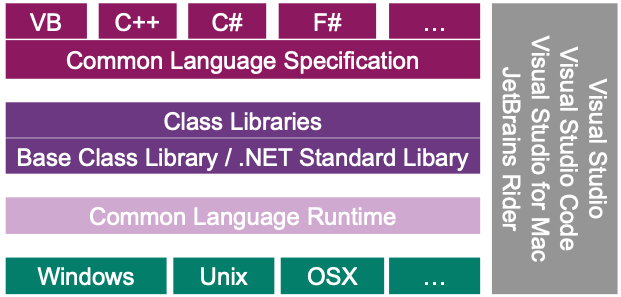
\includegraphics[scale=0.28]{graphic/grundlagen/Grundlagen_dotNET Architektur.png}
\end{center}
\vspace{-8pt}


\subsection{Common Language Runtime(CLR)}
Die CLR ist eine Laufzeitumgebung für .NET-Code, welche ähnlich wie die JVM bei Java ist. Sie umfasst Funktionen wie:\\
\begin{multicols}{2}
\begin{itemize}
    \item JIT-Compilers für die Übersetzung von Intermediate Language Code in Maschinencode
    \item Class Loader für das Laden von Klassen-Code zur Laufzeit
    \item Garbage Collection
    \item Code Access Security
    \item Sprachübergreifendes Debugging
    \item Exceptions
    \item Type Checking und Code Verifikation des IL-Codes
    \item Thread-Verwaltung
    \item Basis-Klassen mit System-Funktionen
\end{itemize}
\end{multicols}

\subsubsection{CLR Architektur}
Die Programmiersprache Visual Basic, C\# sowie C++ werden von einenm Compiler in einen IL Code übersetzt.
Anschliessend wird der IL Code durch die JIT Compiler der Common Language Runtime in eine exe oder dll übersetzt (Maschinencode)
\vspace{-8pt}
\begin{center}
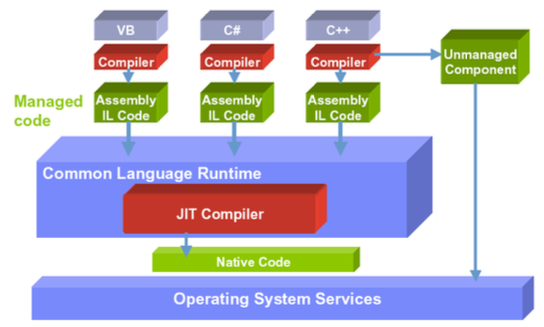
\includegraphics[scale=0.3]{graphic/grundlagen/Grundlagen_CLR Architetktur}
\end{center}

\subsection{Microsoft Intermediate Language (MSIL)}
Die Microsoft Intermediate Language ist eine vorkompilierte Zwischensprache und Prozessor-unabhängig.
Die Sprache an sich selbst sieht sehr Assemblermässig aus.\\
\begin{enumerate}
   \item Portabilität $\rightarrow$ z.B. Nicht-Intel-Prozessoren / Unix / etc.
   \item Typsicherheit $\rightarrow$ Beim Laden des Code können Typen- Sicherheits- und weitere Security-Checks durchgeführt werden.
\end{enumerate}

\begin{enumerate}
   \item Laufzeiteffizienz $\rightarrow$ (kann wettgemacht werden durch JIT-Compiler, welcher zur Laufzeit den Prozessortyp erkennt und spezifische Maschineninstruktionen ausnutzen kann)
\end{enumerate}

    \begin{center}
    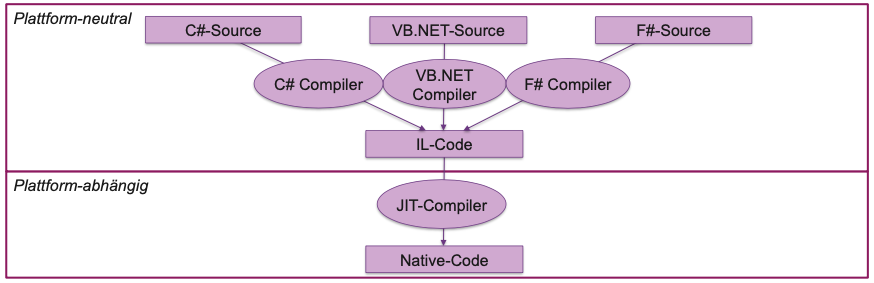
\includegraphics[scale=0.28]{graphic/grundlagen/Grundlagen_MSIL.png}
    \end{center}


\subsubsection{Just in Time (JIT) Compiler}

Die bereits übersetzten Methoden sind in der Grafik mit (ASM) bezeichnet.
Die restlichen Methoden stehen noch als IL Code zur verfügung.
Es wird die Methode 1 in Klasse A ausgeführt.
Diese ruft die Methode 1 in der Klasse B auf.
Anschliessend wird erkannt, dass die Methode 1 in B noch nicht übersetzt wurde.
Der JIT Compiler übersetzt diese Methode dann und übersetzt den IL Code und ersetzt diesen durch Assembler Code.
\begin{center}
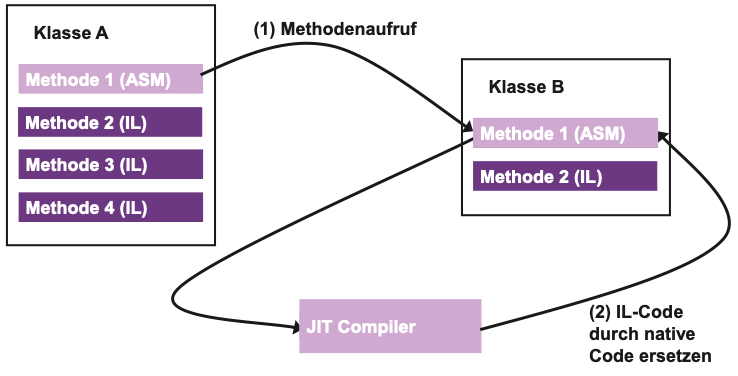
\includegraphics[scale=0.28]{graphic/grundlagen/Grundlagen_JIT Compile.png}
\end{center}


\subsection{Assemblies}
\begin{multicols}{2}
\begin{itemize}
    \item Kompilation erzeugt Assemblies
    \item Deployment- und Ausführungs-Einheit
    \item Executable (*.exe) oder Library (*.dll)
    \item Dynamisch ladbar
    \item Definiert Typ-Scope
    \item Kleinste versionierbare Einheit
\end{itemize}
\end{multicols}

\subsubsection{Überblick}
Ein Assembly besteht hauptsächlich aus 3 Komponenten:





\begin{tabular}{p{2.4cm} | p{2.4cm} | p{2.4cm}}
    \textcolor{OSTPink}{Manifest} & \textcolor{OSTPink}{Module} & \textcolor{OSTPink}{Resourcen}\\
    \hline
    Referenzen $\rightarrow$ welche weiteren Assemblys dieses referenzieren&0 bis n Stück (Können Klassen, Interfaces, Enumerationen, etc. sein)&Bilder, etc.\\
    Metadaten für Klassen und Ressourcen&Typ aus MSIL Code&\\
    Infos $\rightarrow$ Versionsdaten und Autoren Infos& Metadaten (public, abstract etc)&\\
\end{tabular}
\vspace{-8pt}
\begin{center}
\includegraphics[scale=0.3]{graphic/grundlagen/Grundlagen_Assemblies Überblick.png}
\end{center}
\vspace{-8pt}

\subsection{CommonTypeSystem}
\subsubsection{Überblick}
CLR hat ein integriertes Typen-System
\begin{itemize}
    \item Einheitliches Typensystem für alle .NET-Programmiersprachen
    \item Typen in Laufzeitsystem definiert, nicht in Programmiersprache
    \item Alle Typen sind von System.Object abgeleitet
    \item Reference- und Value-Types (int, long, bool, etc.)
    \item Automatische Umwandlung (Value Types – Reference Types)
\end{itemize}

\subsection{Reference- \& Value Types}
    \begin{tabular}{| p{2.5cm}  p{2.5cm} | p{2.5cm}|}

        \hline
        &Reference (Class)&Value(Struct)\\
        \hline
        \hline
        Speicherort&Heap&Stack\\
        \hline
        Variable enthält&Objekt-Referenz&Wert\\
        \hline
        Nullwerte&Möglich&Nie\\
        \hline
        Default value&null&0|false|'\textbackslash0'\\
        \hline
        Methodenaufruf&Kopiert Referenz& Kopiert Wert\\
        \hline
        Ableitung möglich&Ja&Nein (sealed)\\
        \hline
    \end{tabular}




\subsubsection{Reference Types}

    \begin{itemize}
        \item Auf dem Heap gespeichert
        \item Variable enthält Referenz
        \item Garbage Collected
        \item Konstruktor erzeugt \& initialisiert Objekt
        \item Objekt hat Referenz auf seine Typenbeschreibung
    \end{itemize}
\vspace{-8pt}
\begin{center}
    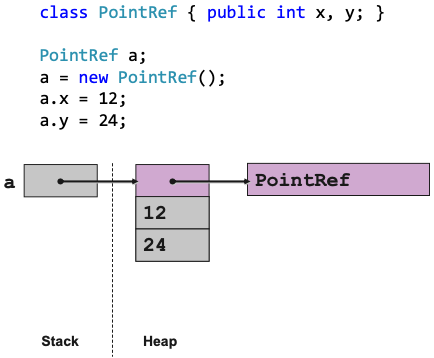
\includegraphics[scale=0.35]{graphic/grundlagen/Grundlagen_Reference Types.png}
\end{center}
\vspace{-8pt}

\subsubsection{Value Types}

\begin{itemize}
    \item Zur Speicherung Roher Werte
    \item Auf Stack abgelegt
    \item Konstruktur macht nur Initialisierung
    \item sealed
    \item Boxing $\rightarrow$ Automatische Umwandlung in Reference Type
    \item Unboxing $\rightarrow$ Automatische Rückumwandlung in Value Type
    \item Effizienter Zugriff
    \item Keine Garbage Collection nötig
    \end{itemize}

\begin{center}
    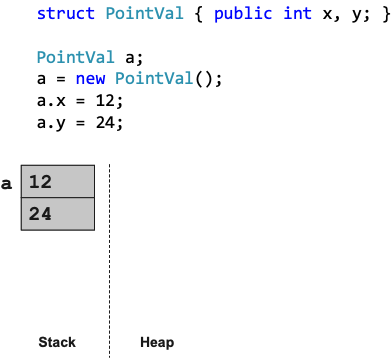
\includegraphics[scale=0.35]{graphic/grundlagen/Grundlagen_Value Types.png}
\end{center}



\subsection{Boxing \& Unboxing}
Vorab den Wert speichern als int:
\begin{lstlisting}
System.Int32 i1 = 123;
\end{lstlisting}


\subsubsection{Boxing}
Kopiert Value Type in einen Reference Type.
\begin{lstlisting}
System.Object obj = i1;
\end{lstlisting}


\subsubsection{Unboxing}
Kopiert Reference Type in einen Value Type.
\begin{lstlisting}
System.Int32 i2 = (System.Int32)obj;
\end{lstlisting}

\vspace{10pt}

Zusammengefasst sieht das ganze Grafisch so aus:
\begin{center}
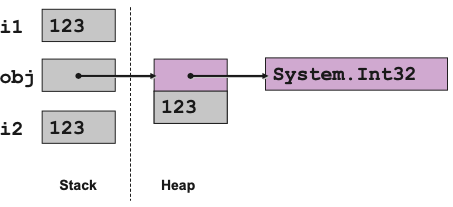
\includegraphics[scale=0.4]{graphic/grundlagen/Grundlagen_Boxing und Unboxing}
\end{center}


\newpage
	%! Author = mariuszindel
%! Date = 02.11.20

\section{C\# Grundlagen}

\subsection{Überblick}
\subsubsection{Syntax}
Neue Code Features:
\begin{itemize}
    \item Referenzparameter
    \item Structs
    \item Blockmatratzen
    \item Enumerationstypen
    \item Uniformes Typsystem (int, long, etc.)
    \item goto $\rightarrow$ schlecht
    \item Systemnahes Programmieren
    \item Versionierung
\end{itemize}
Syntactic Sugar:
\begin{itemize}
    \item Komponentenunterstützung
    \begin{itemize}
        \item Properties
        \item Events
    \end{itemize}
    \item Delegates
    \item Indexers
    \item Boxing / Unboxing
\end{itemize}

\subsection{Sichtbarkeit}
\begin{tabular}{p{1cm} | p{7cm}}
    Attribut & Beschreibung\\
    \hline
    public & Überall sichtbar\\
    private & Innerhalb des jeweiligen Typen sichtbar\\
    protected & Innerhalb des jeweiligen Typen oder abgeleiteter Klasse sichtbar\\
    internal & Innerhalb des Assemblies sichtbar\\
    protected internal & Innerhalb des jeweiligen Typen, abgeleiteter Klasse oder Assemblies sichtbar\\
    private protected & Innerhalb des jeweiligen Typen, abgeleiteter Klasse wenn im gleichen Assemblie\\
\end{tabular}

\begin{tabular}{p{0.8cm} | p{0.8cm}| p{1cm}| p{0.8cm}| p{2.8cm}}
    Typ & Standart & Zulässig & Standart Members & Zulässig Members\\
    \hline
    class&internal&public/ internal&private& public protected internal private protectedinternal privateprotected\\
    struct&internal&public/ internal&private&public internal private\\
    enum&internal&public/ internal&public&-\\
    interface&internal&public/ internal&public&-\\
    delegate&internal&public/ internal&-&-\\
\end{tabular}

\subsection{Namespaces}

\begin{itemize}
    \item Entspricht in Java dem «Package»
    \item Beinhaltet
    \begin{itemize}
        \item Andere Namespaces
        \item Klassen
        \item Interfaces
        \item Structs
        \item Enums
        \item Delegates
    \end{itemize}
    \item Mehrere Namespaces in einem File möglich
    \item Namespace und Ordnerstruktur können sich unterscheiden
\end{itemize}
\begin{lstlisting}
//Es werden Namespaces importiert:
  using System;

//Namespaces werden in andere NS importiert:
namespace A
{ // gilt nur in dieser Datei fuer A
using C; }
namespace B { using D; }

//Alias-Namen moeglich
using F = System.Windows.Forms;
...
F.Button b;
\end{lstlisting}
\vspace{-10pt}
\begin{center}
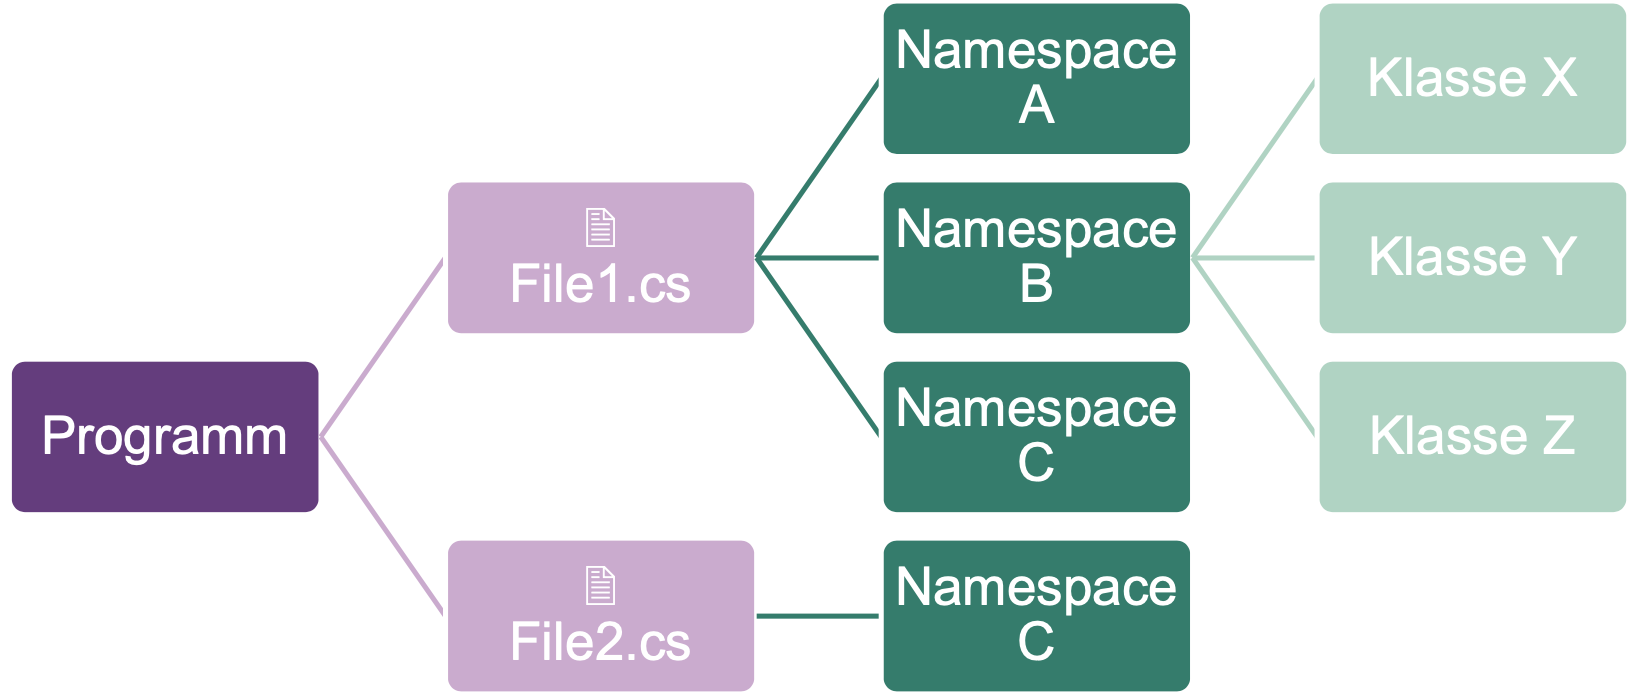
\includegraphics[scale=.21]{graphic/cGrundlagen/CGrundlagen_Aufteilung in Dateien.png}
\end{center}
\vspace{-8pt}

\subsection{Enumerationstypen}
Liste vordefinierter Konstanten inklusive Wert
\begin{lstlisting}
//Deklaration(leitet implizit von Int32 ab)
enum Days { Sunday, Monday, Tuesday, Wednesday, Thursday, Friday, Saturday };

// Verwendung:
Days today = Days.Monday;
if (today == Days.Monday) { /* ... */ } today = Days.Tuesday;
\end{lstlisting}

\subsubsection{Wertedefinition}
\begin{tabular}{l | l | l}
    Sunday&0&Erster Wert erhält 0\\
    Monday&1&Letzter Wert + 1\\
    Tuesday&2&Letzter Wert + 1\\
    Wednesday&3&Letzter Wert + 1\\
    Thursday&4&Letzter Wert + 1\\
    Friday&5&Letzter Wert + 1\\
    Saturday&6&Letzter Wert + 1\\
\end{tabular}
\begin{lstlisting}
// Werteauslesen/interpretieren(Int32)
int sundayValue = (int)Days.Sunday;

Console.WriteLine("{0} / #{1}.", Days.Sunday, sundayValue); // Ausgabe: Sunday / #0
int fridayValue = (int)Days.Friday;
Console.WriteLine("{0} / #{1}.", Days.Friday, fridayValue); // Ausgabe: Friday / #5
\end{lstlisting}

\subsubsection{explizite Wertedefinition}
\begin{lstlisting}
enum Days { Sunday = 10, Monday, Tuesday, Wednesday, Thursday, Friday = 9, Saturday };
\end{lstlisting}

\subsubsection{Basis-Typen}
Vergrössern / Verkleinern Wertebereich \& Speichernutzung:
\begin{lstlisting}
// Deklaration:
enum Days : byte { Sunday, Monday, Tuesday, Wednesday, Thursday, Friday, Saturday };
// Verwendung:
byte today = (byte)Days.Monday;
\end{lstlisting}

\subsubsection{Parsing}
Verwendung der Klasse «Enum»
\begin{lstlisting}
// String zu Enum parsen
Days day1 = (Days)Enum.Parse(typeof(Days), "Monday"); // Non-Generic (Exception on failure)
bool success3 = Enum.TryParse("Monday", out Days day3); // Generic / C# 7.0
\end{lstlisting}


\subsection{Arrays}
\subsubsection{Eindimensionale}
\begin{lstlisting}
int[] a = { 1, 3, 5 };

int length = array1.Length;

int value1 = array1[4];
\end{lstlisting}
\begin{center}
    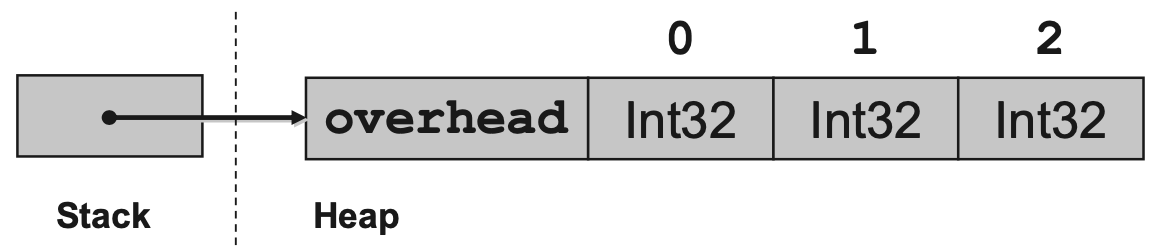
\includegraphics[scale=.23]{graphic/cGrundlagen/CGrundlagen_1Array_ValueTypes.png}
\end{center}
\vspace{-8pt}

\begin{lstlisting}
object[] a = new object[3]; a[1] = new object();
a[2] = 5;
\end{lstlisting}
\begin{center}
    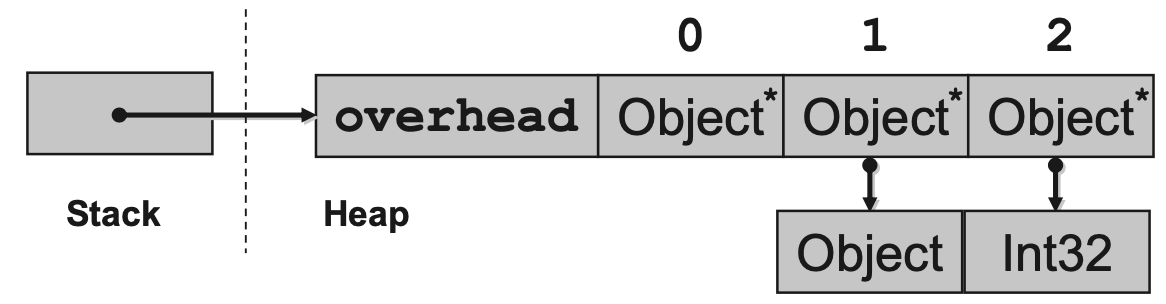
\includegraphics[scale=.23]{graphic/cGrundlagen/CGrundlagen_1Array_ReferenceTypes.png}
\end{center}
\vspace{-8pt}

\subsubsection{Mehrdimensionale (rechteckig / Blockmatritzen)}
\begin{lstlisting}
int[,] a = new int[3,2];
a[0,1] = 9; // Schreiben
int x = a[0,1]; // Lesen / Liefert 9

int length = a.Length; // Liefert 6
int length0 = a.GetLength(0); // Liefert 3
int length1 = a.GetLength(1);// Liefert 2
\end{lstlisting}
\begin{center}
    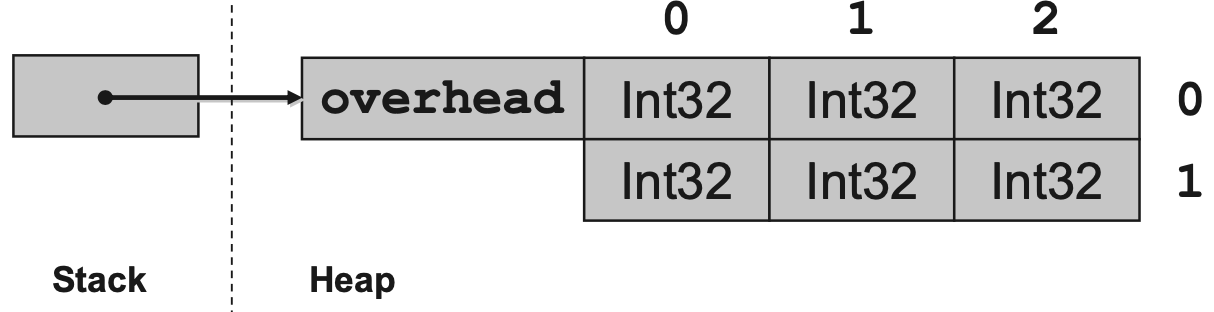
\includegraphics[scale=.23]{graphic/cGrundlagen/CGrundlagen_MArray_Rechteckig.png}
\end{center}
\vspace{-8pt}

\subsubsection{Mehrdimensionale (jagged)}
\begin{lstlisting}
int[][] a = new int[2][];
a[0] = new int[2];
a[1] = new int[1];
a[0][1] = 9; // Schreiben
int x = a[0][1]; // Lesen / Liefert 9

int length = a.Length; // Liefert 2
int length0 = a[0].Length; // Liefert 2
int length1 = a[1].Length; // Liefert 1
\end{lstlisting}
\begin{center}
    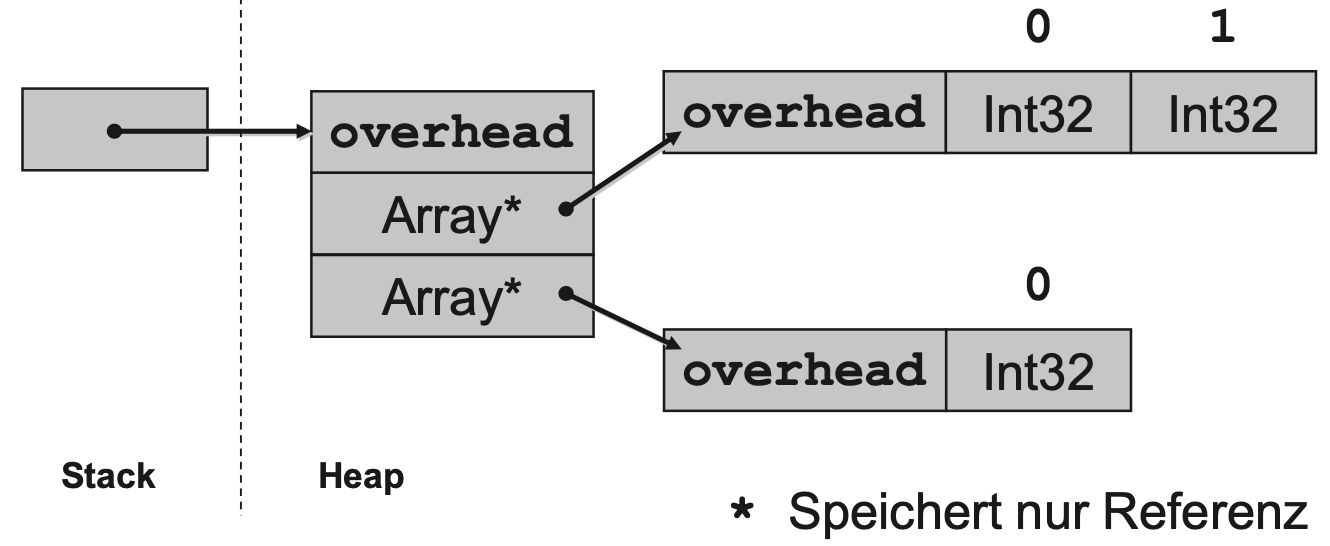
\includegraphics[scale=.23]{graphic/cGrundlagen/CGrundlagen_MArray_Jagged.png}
\end{center}
\vspace{-8pt}

\subsubsection{Vor-/Nachteile Blockmatritzen}
\begin{itemize}
    \item Speicherplatz-Effizienz
    \item SchnelleresAllozieren
    \item Schnellere Garbage Collection da «en bloc»
    \item Aber Boundary-Check wird bei 1-dimensionalen Arrays optimiert (gilt nicht für Blockmatrizen)
\end{itemize}

\subsection{Typkompatibilität}
\begin{center}
    \includegraphics[scale=.23]{graphic/cGrundlagen/CGrundlagen_Typkompatibilität.png}
\end{center}
\vspace{-8pt}

\subsection{Jumps}
\begin{itemize}
    \item break $\rightarrow$ Aktuellen Loop beenden
    \item continue $\rightarrow$ Zur nächsten Loop-Iteration
    \item goto «label» $\rightarrow$ Sprung zu «label»
\end{itemize}

\newpage
	%! Author = mariuszindel
%! Date = 02.11.20

\section{Klassen \& Structs}

\subsection{Klassen}
\begin{itemize}
    \item Reference Type $\rightarrow$ Auf dem Heap angelegt
    \item Vererbung
    \begin{itemize}
        \item Ableitung von Basisklasse möglich
        \item Implementation von Interfaces möglich
    \end{itemize}
    \item wird mit new instanziiert
    \item Deklaration
    \begin{itemize}
        \item Konstruktoren: Parameter optional
        \item Felder: Initialisierung erlaubt
    \end{itemize}
\end{itemize}

\begin{lstlisting}
class Stack {
    int[] values;
    int top = 0;

    public Stack(int size) { /* ... */ }

    public void Push(int x) { /* ... */ }
    public int Pop() { /* ... */ }
}
\end{lstlisting}

\subsection{Structs}
\begin{itemize}
    \item Value Type $\rightarrow$ Auf dem Stack angelegt oder «in-line» in einem Objekt auf dem Heap
    \item Vererbung
    \begin{itemize}
        \item Ableiten von Basisklasse nicht möglich
        \item Implementation von Interfaces möglich
    \end{itemize}
    \item wird mit new instanziiert
    \item Deklaration
    \begin{itemize}
        \item Konstruktoren: mind. 1 Parameter
        \item Felder: Initialisierung nicht erlaubt!
    \end{itemize}
\end{itemize}

\begin{lstlisting}
struct Point {
    int x;
    int y;

    public Point(int x, int y) {
        this.x = x; this.y = y;
    }
    public void MoveX(int x) { /* ... */ }
    public void MoveY(int y) { /* ... */ }
}
\end{lstlisting}

Ein Struct sollte nur unter folgenden Umständen verwendet werden:
\begin{itemize}
    \item Repräsentiert einen einzelnen Wert
    \item Instanzgrösse ist kleiner als 16 Byte (128 Bit)
    \item Ist “immutable”
    \item Wird nicht häufig geboxt
    \item Kurzlebig oder in andere Objekte eingebettet
\end{itemize}

In allen anderen Fällen sollte eine Klasse verwendet werden!

\subsubsection{Felder}
\begin{itemize}
    \item Initialisierung in Deklaration optional (ausser Struct)
    \item In Deklarationsreihenfolge initialisiert
    \item Initialisierung darf nicht auf Felder und Methoden zugreifen
    \item Struct-Felder dürfen nicht initialisiert werden
    \item Konstante muss Initialisierungswert haben und zur Compilezeit berechenbar sein
\end{itemize}

\begin{lstlisting}
class MyClass {
    int value = 0;
    const long size = int.MaxValue / 3 + 1234;
    readonly DateTime date1 = DateTime.Now;
    readonly DateTime date2;

    public MyClass() {
        date2 = DateTime.Now;
    }

    public void DoSomething() {
        value = 10;
        date2 = DateTime.Now; // Compilerfehler
    }
}
\end{lstlisting}


\subsubsection{Nested Types}
Für spezifische Hilfsklassen gedacht. Regeln:
\begin{itemize}
    \item Äussere Klasse hat Zugriff auf innere Klasse $\rightarrow$ Nur auf «Public Members»
    \item Innere Klasse hat Zugriff auf äussere Klasse $\rightarrow$ Auch auf «Private Members»
    \item Fremde Klassen erhalten Zugriff auf innere Klasse, wenn diese «public» ist
    \item Erlaubte Nested Types sind: Klassen, Interfaces, Structs, Enums, Delegates
\end{itemize}
\begin{lstlisting}
class OuterClass {
    private int outerValue;
    InnerClass innerInstance = new InnerClass();

    public void OuterMethod()
    { innerInstance.InnerMethod(this); }

    public class InnerClass {
        public void InnerMethod(OuterClass outerClass)
        { outerClass.outerValue = 123; } }
    }

// Anwendung
OuterClass outer = new OuterClass();
outer.OuterMethod();

OuterClass.InnerClass inner = new OuterClass.InnerClass();
inner.InnerMethod(outer);
\end{lstlisting}


\subsection{Methoden}
\subsubsection{Parameter Arten}
\paragraph{call by value}
\begin{itemize}
    \item Value-Parameter (call by value)
    \item Kopie des Stack-Inhaltes wird übergeben (Wert oder Heap-Referenz)
\end{itemize}
\begin{lstlisting}
void IncVal(int x) { x = x + 1; } void TestIncVal()
{
int value = 3;
IncVal(value); // value == 3 }
\end{lstlisting}

\paragraph{ref (call by reference)}
\begin{itemize}
    \item ref-Parameter (call by reference)
    \item Adresse der Variable «value» wird übergeben
    \item Variable «value» muss initialisiert sein
    \item Es muss eine Variable übergeben werden
\end{itemize}
\begin{lstlisting}
void IncRef(ref int x) { x = x + 1; } void TestIncRef()
{
int value = 3;
IncRef(ref value); // value == 4
    // Praxisbeispiel (Initialisierungen)
VectorStruct v = new VectorStruct();
    SetToZero(ref v);
}
\end{lstlisting}


\paragraph{out}
\begin{itemize}
    \item Wie ref-Parameter, aber zur Initialisierung von Werten gedacht
    \item Müssen initialisiert werden
    \item Darf in «Init» erst nach Wertzuweisung verwendet werden
    \item Variablen «a» / «b» dürfen initialisiert sein
    \item Nicht benötigte out-Parameter können mit Underscore «out \_» ignoriert werden
\end{itemize}


\begin{lstlisting}
void Init(out int a, out int b) { a = 1; b = 2; }

void TestInit() {

    // C# 7.0 regulaer
    Init(out int a1, out int b1); Console.WriteLine($"{a1} / {b1}");

    // C# 7.0 Parameter ignoriert
    Init(out int a2, out _); Console.WriteLine($"{a1}");
}
\end{lstlisting}

\paragraph{params}
Params-Array:
\begin{itemize}
    \item Erlaubt beliebig viele Parameter (0 – n)
    \item Muss am Schluss der Deklaration stehen
    \item Nur ein params-Array erlaubt
    \item Wird in «Sum» wie ein Array verwendet
    \item params darf nicht mit ref / out kombiniert werden
\end{itemize}
\begin{lstlisting}
void Sum(out int sum, params int[] values) {
    sum = 0;
    foreach (int i in values) sum += i;
}
\end{lstlisting}

\paragraph{OptionaleParameter}
\begin{itemize}
    \item Ermöglicht Zuweisung eines Default-Values
    \item Deklaration muss hinter erforderlichen Parametern erfolgen
    \item Muss zur Kompilierzeit berechenbar sein
    \item Weglassen nur am Ende erlaubt!
\end{itemize}
\begin{lstlisting}
private void Sort( int[] array, // Erforderlich
int from = 0,                   // Optional
int to = -1,                    // Optional
bool ascending = true,          // Optional
bool ignoreCase = false         // Optional
) { ... }
\end{lstlisting}


\subsection{Properties}
\begin{itemize}
    \item Kurzform für Get- / Set- Methoden
    \item Reines Compiler-Konstrukt
    \item Verhält sich wie «Public Field»
\end{itemize}

\begin{lstlisting}
class MyClass {
// Backing-Field
    private int length;
// Property
    public int Length
    {
        get { return length; }
        set { length = value; }
}
\end{lstlisting}
\subsection{Indexer}

Klasse verhält sich wie ein Array

\begin{lstlisting}
class MyClass {
    private string[] arr = new string[10];
    public string this[int index] {
        get { return arr[index]; }
        set { arr[index] = value; }
}

// Verwendung:
MyClass mc = new MyClass();
mc[0] = "Hello";
string value1 = mc[0]; // Hello
\end{lstlisting}


\subsection{Konstruktoren}
\begin{itemize}
    \item Bei jedem Erzeugen einer Klasse / eines Structs verwendet (Aufruf von «new»)
    \item Default - Konstruktor (ohne Parameter) wird generiert, falls nicht kein Konstr. definiert
    \item Statische und nicht- statische Konstruktoren
    \item Konstruktoren können überladen werden
    \item Aufruf anderer Konstruktoren möglich: «this»
    \item Aufruf auf Basis-Klassen-Konstruktor: «base»
\end{itemize}

\begin{lstlisting}
class MyClass {
    private int x, y;

    public MyClass() : this(0, 0) { }
    public MyClass(int x) : this(x, 0) { }
    public MyClass(int x, int y) {
        this.y = y;
        this.x = x; }
}
\end{lstlisting}
\subsubsection{Default Konstruktor}
\begin{multicols}{2}
    \paragraph{Klasse}
    \begin{itemize}
        \item Automatisch generiert wenn nicht vorhanden
        \item Ohne Parameter
        \item Wird nicht generiert, wenn anderer Konstruktor vorhanden
        \item Kann manuell implementiert werden
        \item Konstruktor kann beliebig viele Felder initialisieren
    \end{itemize}
    \vfill
    \columnbreak
    \paragraph{Struct}
    \begin{itemize}
        \item Immer automatisch generiert
        \item Ohne Parameter
        \item Wird auch generiert, wenn anderer Konstruktor vorhanden
        \item Kann nicht manuell definiert werden
        \item Konstruktur muss alle Felder initialisieren (sonst Compilerfehler)
    \end{itemize}
\end{multicols}
\vspace{-8pt}
\begin{center}
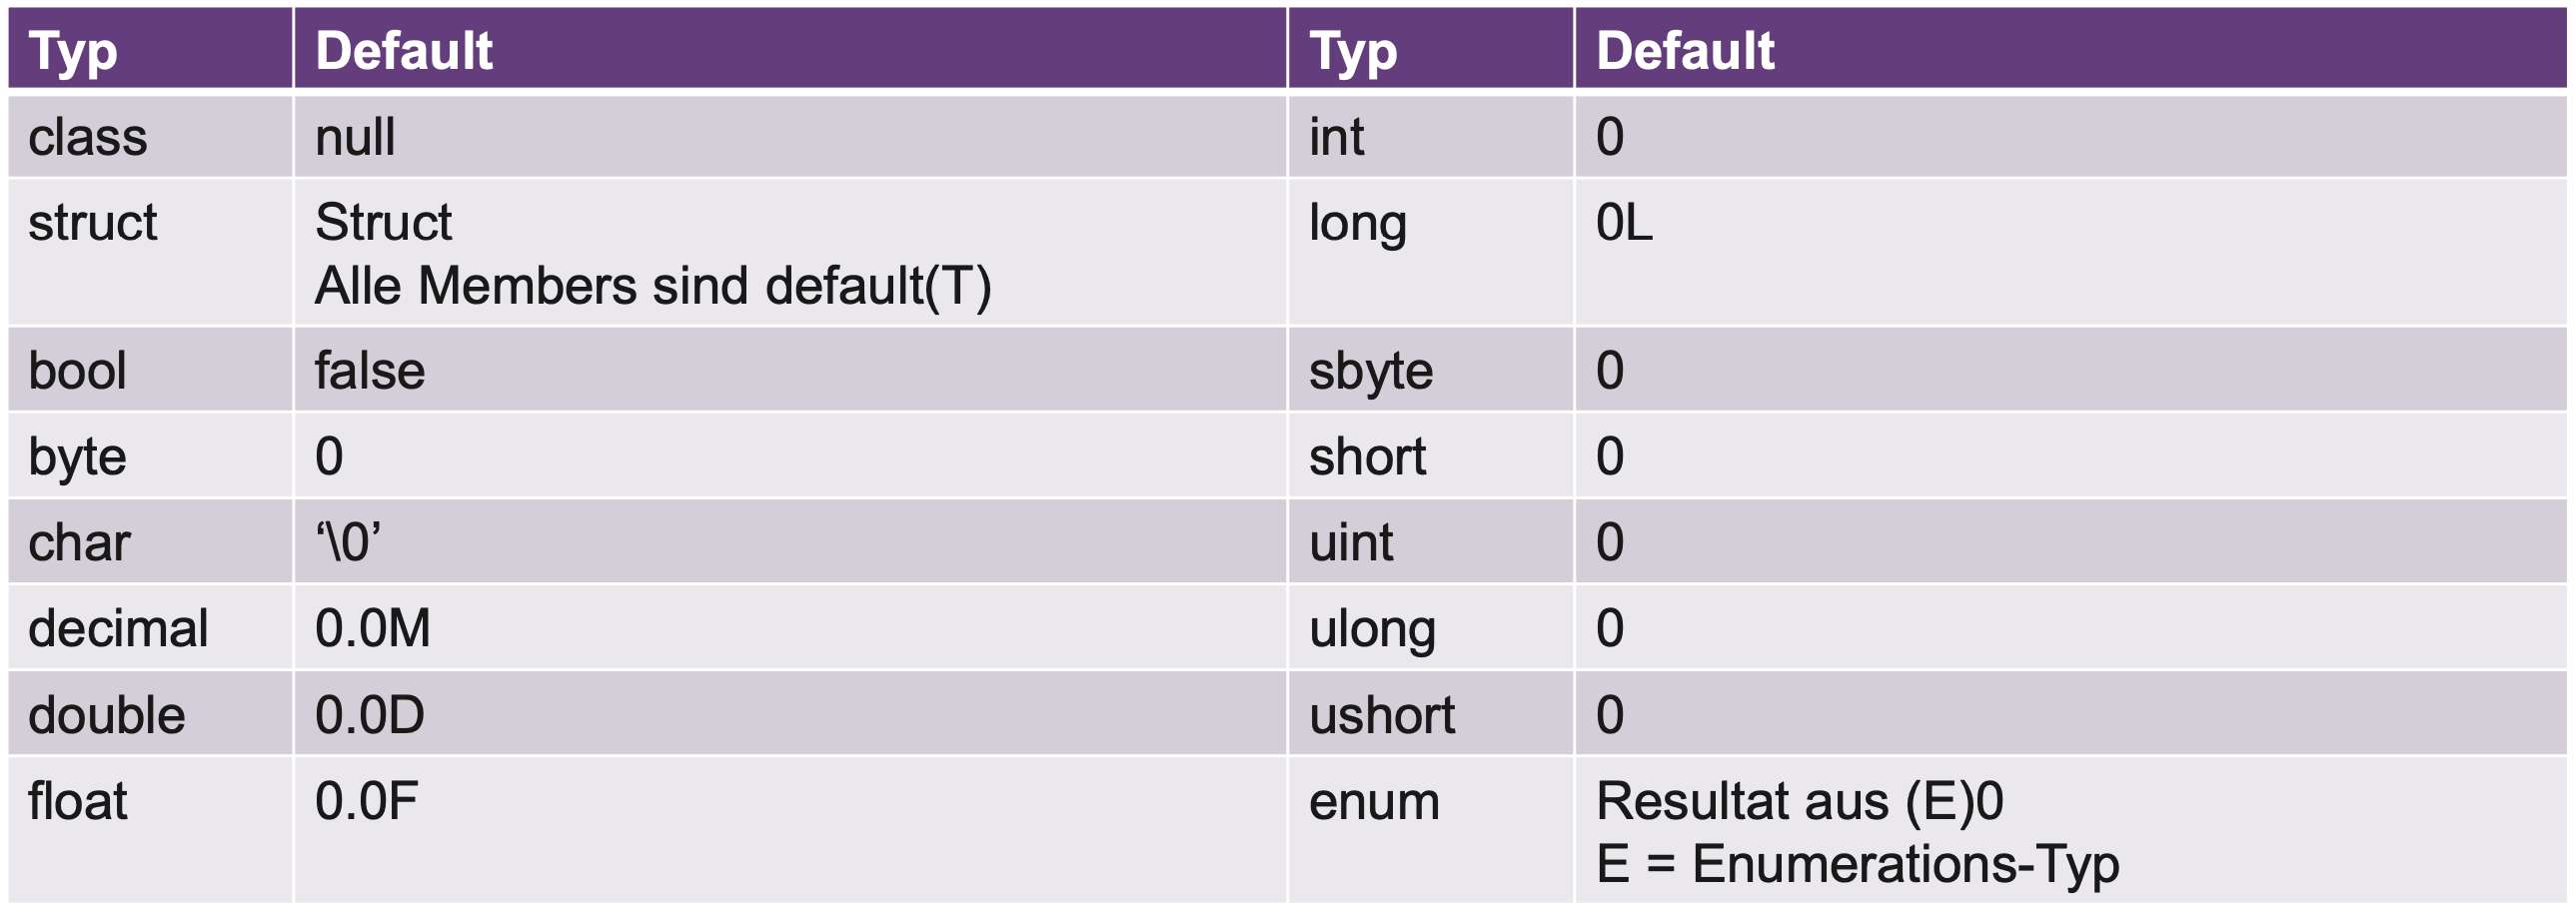
\includegraphics[scale=.18]{graphic/klassen/K&S_Standard-Werte.png}
\end{center}
\vspace{-8pt}

\subsubsection{Statische Konstruktoren}
\begin{itemize}
    \item Zwingend parameterlos
    \item Sichtbarkeit darf nicht angegeben werden
    \item Nur ein statischer Konstruktor erlaubt
    \item Wird genau einmal ausgeführt
    \item Kann nicht explizit aufgerufen werden
\end{itemize}

\subsubsection{Destruktoren}
\begin{itemize}
    \item Ermöglichen Abschlussarbeiten beim Abbau eines Objekts
    \item Nur bei Klassen erlaubt, bei Structs verboten
    \item Zwingend parameterlos / ohne Sichtbarkeit
    \item Nur ein Destruktor erlaubt
    \item Wird vom Garbage Collector aufgerufen
\end{itemize}

\begin{lstlisting}
class MyClass {
~MyClass() {
...
} }
\end{lstlisting}


\subsubsection{Initialisierungs Reihenfolge (ohne Vererbung)}
\begin{lstlisting}
class Base {
    private static int baseStaticValue = 0; private int baseValue = 0;
    static Base() { }
    public Base() { }
}

Base b1 = new Base();
// Base > baseStaticValue
// Base > Statischer Konstruktor
// Base > baseValue
// Base > Konstruktor

Base b2 = new Base();
// Base > baseValue
// Base > Konstruktor
\end{lstlisting}
\subsubsection{Initialisierungs Reihenfolge (mit Vererbung)}
\begin{lstlisting}
class Base {
    private static int baseStaticValue = 0; private int baseValue = 0;
    static Base() { }
    public Base() { }
}
class Sub : Base {
    private static int subStaticValue = 0; private int subValue = 0;
    static Sub() { }
    public Sub() { }
}

Sub s1 = new Sub();
// Sub > subStaticValue
// Sub > Statischer Konstruktor
// Sub > subValue
// Base > baseStaticValue
// Base > Statischer Konstruktor
// Base > baseValue
// Base > Konstruktor
// Sub > Konstruktor

Sub s2 = new Sub();
// Sub > subValue
// Base > baseValue
// Base > Konstruktor
// Sub > Konstruktor
\end{lstlisting}
\vspace{-8pt}
\begin{center}
    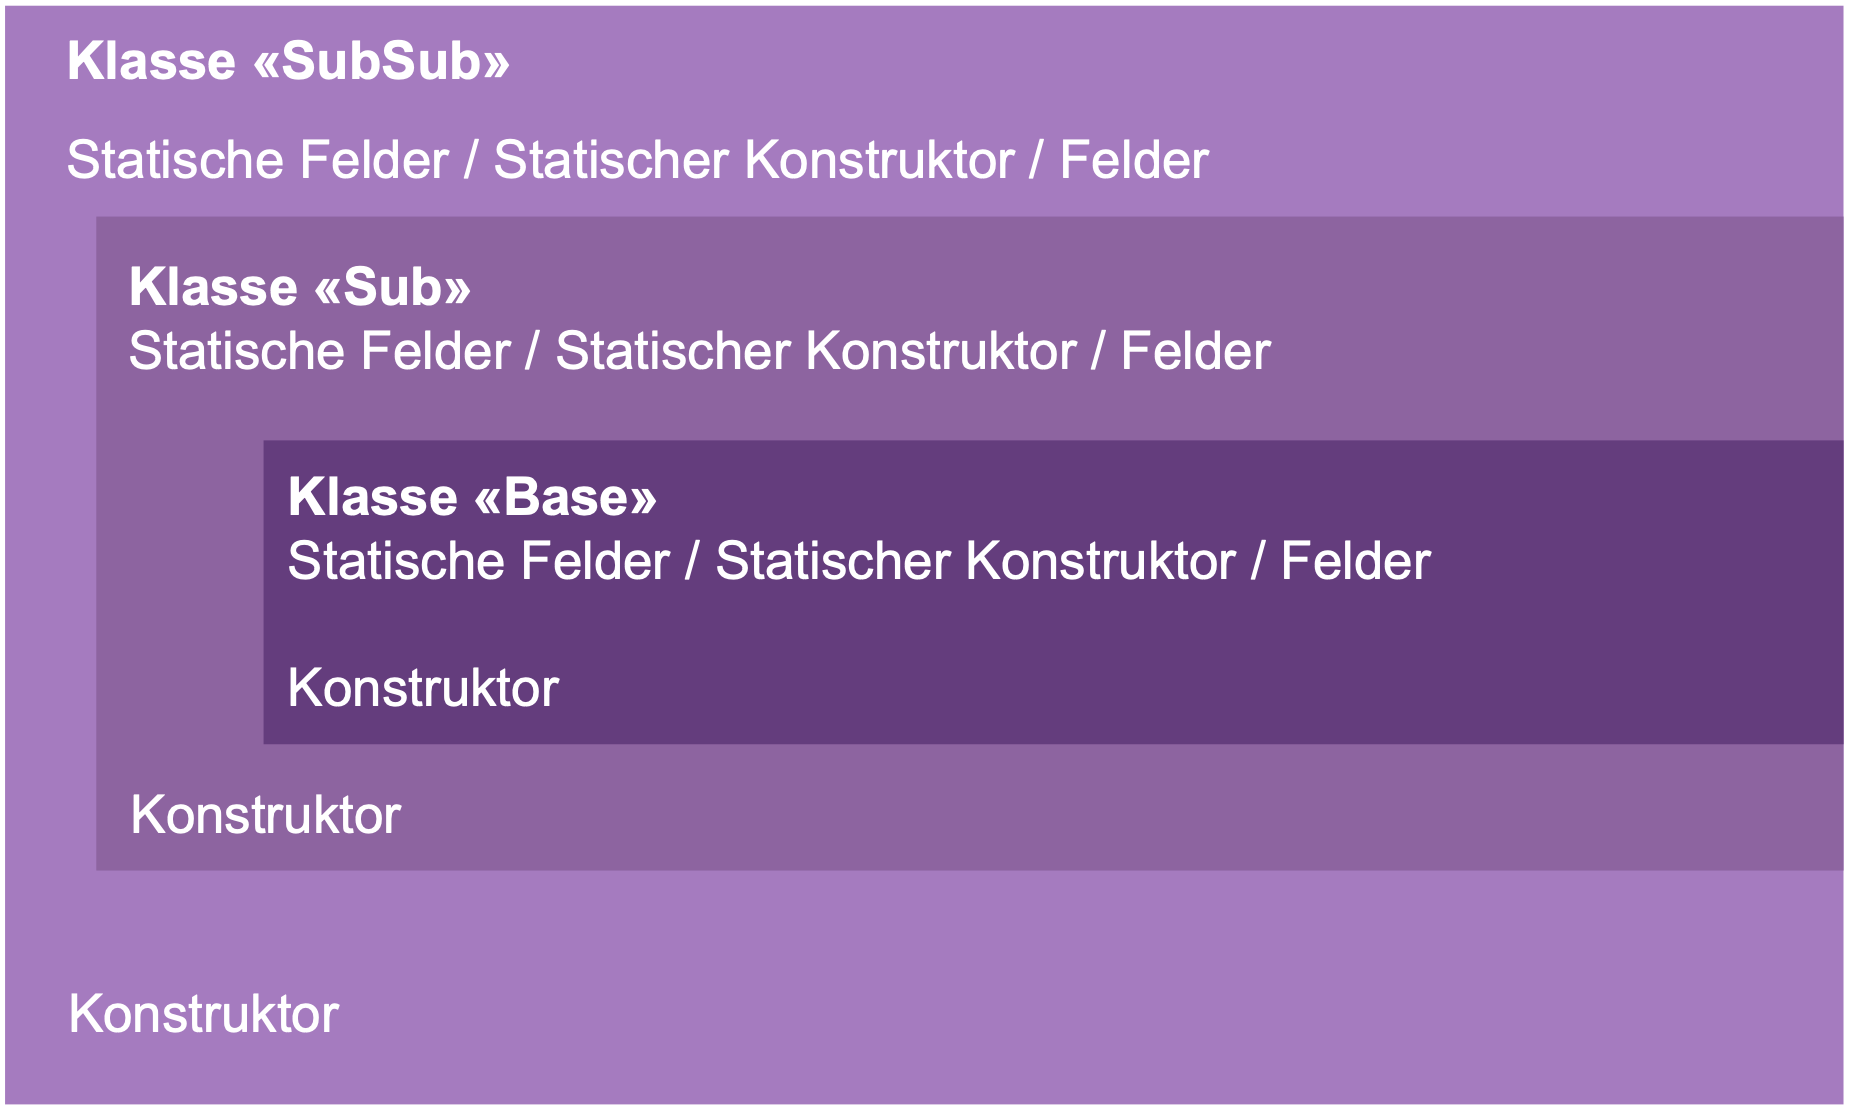
\includegraphics[scale=.2]{graphic/klassen/K&S_Init.png}
\end{center}
\vspace{-8pt}
\subsubsection{Konstruktoren in Ober- und Unterklasse}
\begin{center}
    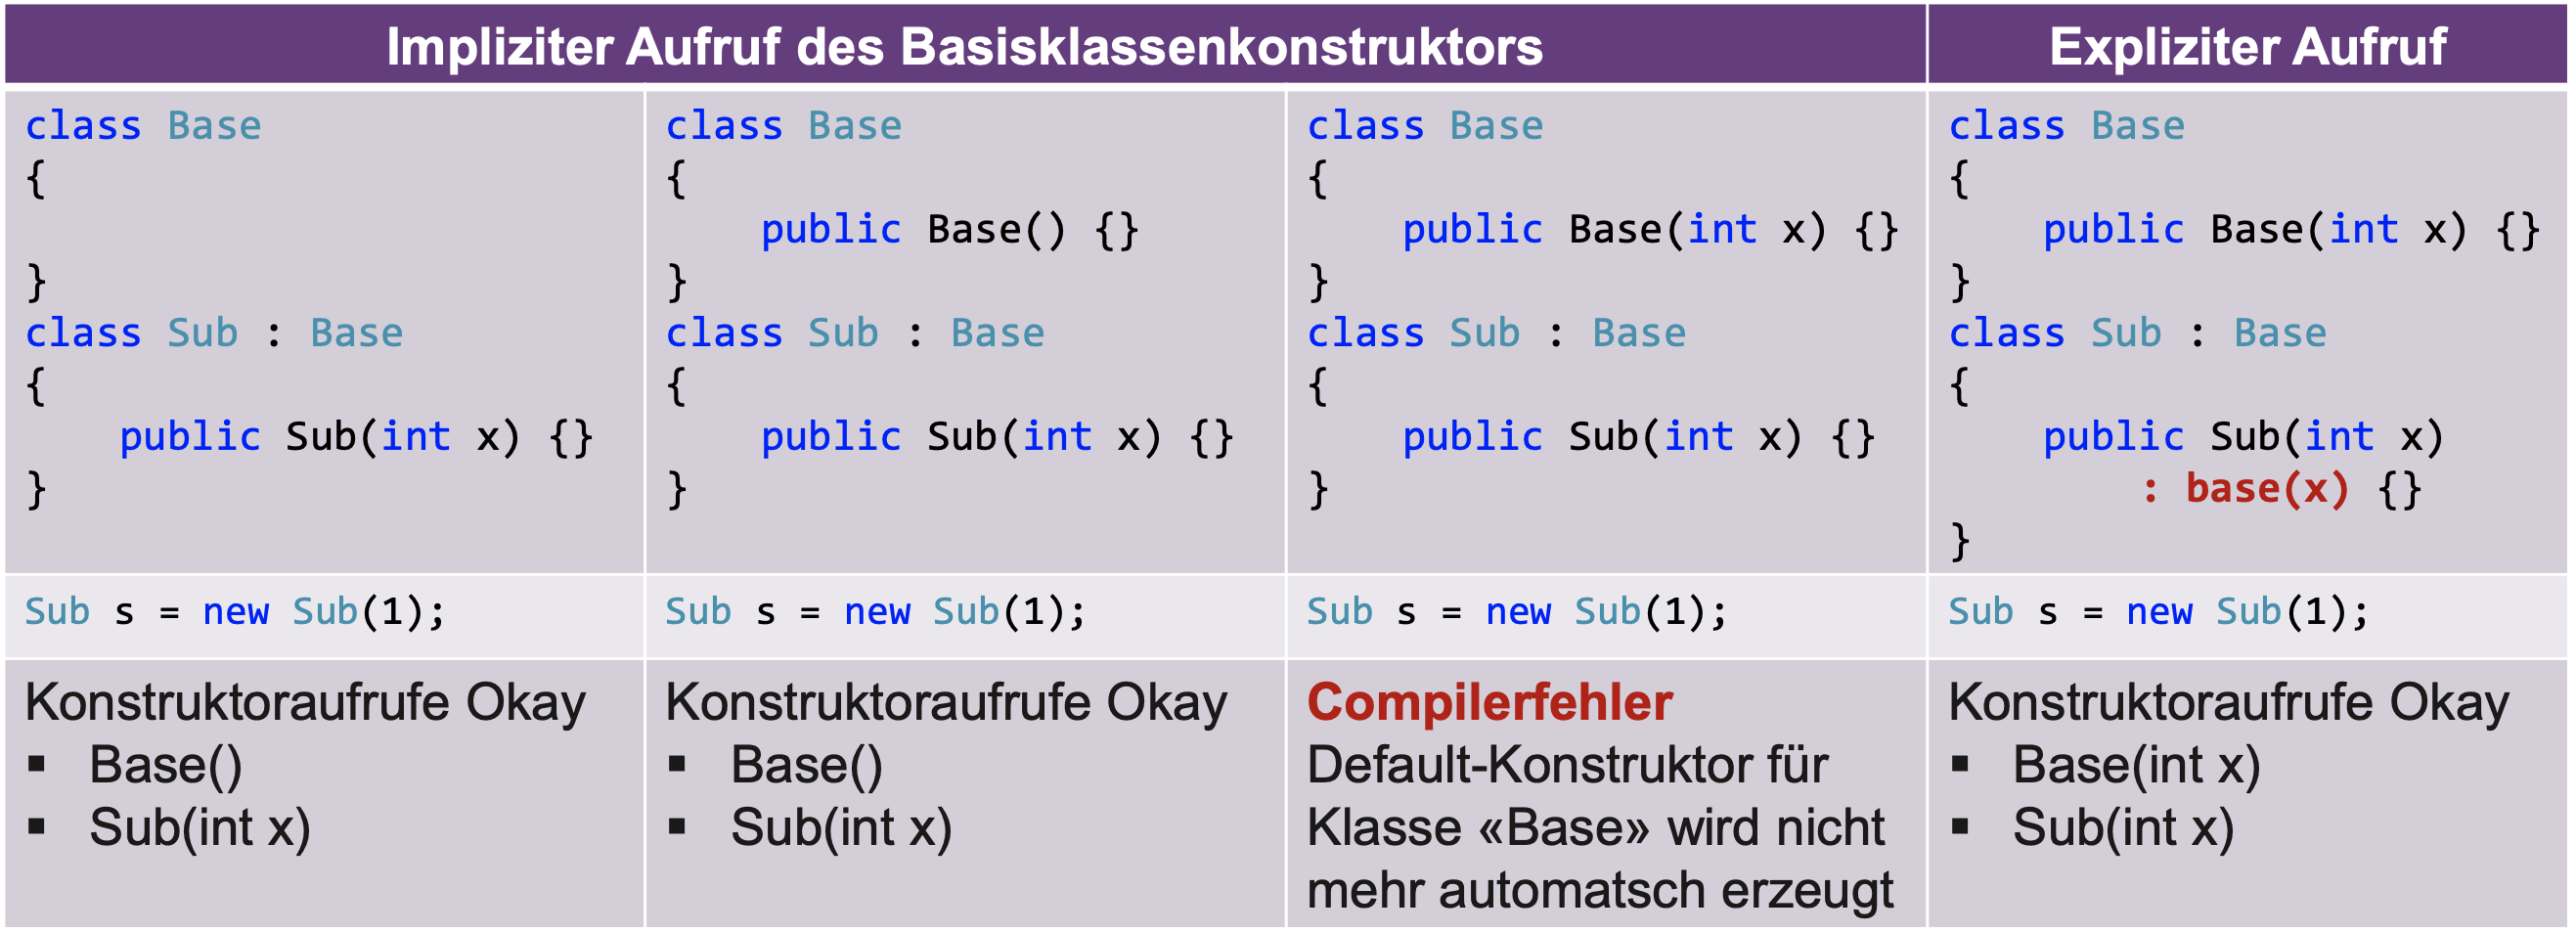
\includegraphics[scale=.19]{graphic/klassen/K&S_Konstruktoren in Ober- und Unterklasse.png}
\end{center}
\vspace{-8pt}


\subsection{Operator Overloading}
\begin{itemize}
    \item Methode muss «static» sein
    \item Schlüsselwort «operator» gefolgt von z.B. +
    \item Unäre Operatoren haben 1 Parameter
    \item Binäre Operatoren haben 2 Parameter
    \item Rückgabetyp ist frei wählbar
    \item Mindestens 1 Parameter muss vom Typ der enthaltenden Klasse sein
\end{itemize}

\begin{lstlisting}
class Point {
    private int x, y;
    public Point(int x, int y) { this.x = x; this.y = y; }

    public static Point operator ~(Point a) {
        return new Point(a.x * -1, a.y * -1); }

    public static Point operator +
        (Point a, Point b) {
        return new Point(a.x + b.x, a.y + b.y);
} }
\end{lstlisting}
\subsubsection{Unäre Operatoren}
\begin{lstlisting}
public static Point operator ~(Point a) {
    return new Point(a.x * -1, a.y * -1);
}

//Verwendung:
Point mcNeg = ~mc;
\end{lstlisting}
\subsubsection{Binäre Operatoren}
\begin{lstlisting}
public static Point operator +
        (Point a, Point b){
    return new Point(a.x + b.x, a.y + b.y);
}

//Verwendung:
Point mcSum = mc1 + mc2;
\end{lstlisting}

\subsection{Partielle Klassen}
\begin{itemize}
    \item Definition eines Typen in meheren Files
    \item Funktioniert mit: Klassen, Structs, Interfaces
    \item Alle Teile müssen die gleichen Sichtbarkeitsattribute haben (z.B. «public»)
    \item «partial» muss bei allen Teilen angemerkt sein
\end{itemize}

\begin{lstlisting}
// File1.cs
partial class MyClass {
    public void Test1() { }
}
// File2.cs
partial class MyClass {
    public void Test2() { }
}
\end{lstlisting}


\subsection{Partielle Methoden}

\begin{itemize}
    \item Trennung von Deklaration und Implementation einer Methode
    \item Ermöglicht Benutzer-definierte «Hooks» in generiertem Code
    \item Funktioniert in Klassen / Structs
    \item Rückgabewert muss «void» sein
    \item Implizit immer «private»
    \item Können «static» sein
\end{itemize}

\begin{lstlisting}
// File1.cs
partial class MyClass {
    public void Test1()
    {
        Test1Initialize();
/* ... */
Test1Cleanup(); }
    partial void Test1Initialize();
    partial void Test1Cleanup();
}
// File2.cs
partial class MyClass
{
    public void Test2() { }
    partial void Test1Initialize() { /* */ }
}
\end{lstlisting}

\newpage
	%! Author = mariuszindel
%! Date = 02.11.20

\section{Vererbung}

\subsection{Überblick}
\begin{itemize}
    \item Nur eine Basisklasse erlaubt
    \item Beliebig viele Interfaces erlaubt
    \item Structs können nicht erweitert werden
    \item Structs können nicht erben
    \item Structs können nur Interfaces implementieren
    \item Klassen sind direkt / indirekt von System.Object abgeleitet
    \item Structs sind über Boxing mit System.Object kompatibel
\end{itemize}
\subsubsection{Zuweisungen}
Zuweisung immer möglich wenn
\begin{itemize}
    \item Statischer Typ gleich Dynamischer Typ
    \item Statischer Typ Basisklasse von Dynamischem Typen
\end{itemize}
Zuweisung verboten wenn
\begin{itemize}
    \item Statischer Typ Subklasse von Dynamischem Typen
    \item Statischer Typ und Dynamischer Typ nicht in der gleichen Vererbungshierarchie sind
\end{itemize}
\begin{lstlisting}
class Base { }
class Sub : Base { }
class SubSub : Sub { }

public static void Test()
{
// Statischer Typ: Base
// Dynamischer Typ: Base
    Base b = new Base();

// Dynamischer Typ: Sub
    b = new Sub();

// Dynamischer Typ: SubSub
    b = new SubSub();

// Compilerfehler (Typecast)
    Sub s = new Base();
    }
\end{lstlisting}
\subsubsection{Typprüfungen}
Prüft ob ein Objekt mit einem Typen kompatibel ist $\rightarrow$ Liefert bool\\

Liefert true wenn:
\begin{itemize}
    \item Typ von «obj» identisch wie «T» ist
    \item Typ von «obj» eine Sub-Klasse von «T» ist
\end{itemize}
Liefert false wenn
\begin{itemize}
    \item «obj» null ist
    \item Typ von «obj» eine Basisklasse von «T» ist
    \item Typ von «obj» und «T» nicht in der gleichen Vererbungshierarchie sind
\end{itemize}
\begin{lstlisting}
if (a is SubSub) { /* ... */ }
\end{lstlisting}

\subsubsection{Type Casts}
Explizite Typumwandlung als Hinweis für den Compiler
\begin{itemize}
    \item Anweisung an Compiler, einen Typen in einen anderen umzuwandeln
    \item null kann auch gecastet werden
    \item Compilerfehler wenn erkennbar, dass Type Cast nicht zulässig
    \item Compilerfehler wenn erkennbar, dass null in einen Value Type gecastet wird
    \item Laufzeit-Fehlverhalten: InvalidCastException
\end{itemize}
\begin{lstlisting}
Sub s = (Sub)b;
\end{lstlisting}

\subsubsection{Type Casts mit as-Operator}
ExpliziteTypumwandlungals Hinweis für den Compiler
\begin{itemize}
    \item Syntactic Sugar / Compiler erzeugt «obj is T ? (T)obj : (T)null»
    \item Laufzeit-Fehlverhalten: null
\end{itemize}
\begin{lstlisting}
Sub s = b as Sub;
\end{lstlisting}

\subsubsection{Typprüfungen mit implizitem Type Cast}
PrüftobeinObjektmiteinemTypen kompatibel ist
\begin{itemize}
    \item Syntax: «obj is T result»
    \item Variable «result» vom Typ «T» enthält gecasteten Wert
    \item Funktioniert wie normaler Type Cast
    \item Arbeitet nicht mit Nullable Types im Gegensatz zu «as»
\end{itemize}
\begin{lstlisting}
Base a = new SubSub();
if (a is SubSub casted) {
Console.WriteLine(casted); }
\end{lstlisting}


\subsection{Methoden \& Vererbung}
\subsubsection{Methoden überschreiben}
Subklasse kann Members der Basisklasse überschreiben.\\
$\rightarrow$ Schlüsselwörter «virtual» und «override»

\begin{itemize}
    \item Basisklasse:\\
    «virtual» um Basis-Methode überschreibbar zu machen
    \item Subklasse:\\
    «override» um Basis-Methode zu überschreiben
\end{itemize}
\begin{lstlisting}
class Base {
public virtual void G() { /* ... */ } }
class Sub : Base
{
public override void G() { /* ... */ } }
\end{lstlisting}
Regeln:
\begin{itemize}
    \item Members sind per Default NICHT «virtual»
    \item Members sind per NICHT «overrride»
    \item Signatur muss identisch sein
\end{itemize}

\subsubsection{Methoden überdecken}
\begin{itemize}
    \item Unterbricht Dynamic Binding!
    \item Subklasse kann Members der Basisklasse überdecken
\end{itemize}
\subsubsection{Methoden überdecken mit «new»}
\begin{itemize}
    \item Compiler warnung kann mit «new» Schlüsselwort vermieden werden
    \item Hinweis für Compiler, dass Member bewusst überdeckt wurde
\end{itemize}
\begin{lstlisting}
class Base {
public virtual void I() { /* ... */ } }
class Sub : Base
{
public override void I() { /* ... */ } }
class SubSub : Sub
{
public new void I() { /* ... */ }
public new void I2() { /* ... */ } }
\end{lstlisting}

\subsubsection{Dynamic Binding / Regelwerk komplett in Pseudocode}
Suche Vererbungs-Hierarchie von oben nach unten nach konkretester Methode «G()» mit Schlüsselwort «override»


\subsection{Abstrakte \& Versiegelte Klassen}
\subsubsection{Abstrakte Klassen}
\begin{itemize}
    \item Mischung aus Klasse und Interface
    \item Kann nicht direkt instanziert werden
    \item Kann beliebig viele Interfaces implementieren
\end{itemize}
\begin{lstlisting}
abstract class Sequence {
public abstract void Add(object x); // Method
public abstract string Name { get; } // Prop.
public abstract object this[int i] // Idx.
{ get; set; }
public abstract event EventHandler OnAdd;
                                         // Event

public override string ToString() { return Name; }
}
class List : Sequence
{
public override void Add(object x) { /* ... */ }
public override string Name
{ get { /* ... */ } }
public override object this[int i]
{ get { /* ... */ } set { /* ... */ } } public override event EventHandler OnAdd;}
\end{lstlisting}
\subsubsection{Abstrakte Methoden}
\begin{itemize}
    \item Kein Anweisungsteil
    \item Sind implizit virtual
    \item Dürfen nicht «static» oder «virtual» sein
\end{itemize}
\subsubsection{Abstrakte Properties / Indexer}
\begin{itemize}
    \item Kein Anweisungsteil
    \item Sind implizit virtual
    \item Dürfen nicht «static» oder «virtual» sein
    \item «get» und «set» Kombination muss bei Implementation identisch sein
\end{itemize}

\subsubsection{Versiegelte Klassen}
\begin{itemize}
    \item Verhindert das Ableiten einer Klasse
    \item Analog «final» bei Java
    \item Sicherheitsaspekte verhindert versehentliches Erweitern
\end{itemize}

\begin{lstlisting}
sealed class Sequence {
    public void Add(object x) {}
    public string Name { get{} }
    public object this[int i] { get{} }
    public event EventHandler OnAdd;
}
// Compilerfehler
class List : Sequence { /* ... */ }
\end{lstlisting}


\subsubsection{Versiegelte Members}
\begin{itemize}
    \item Verhindert das Überschreiben eines bestimmten Members
    \item Muss in Kombination mit «override» angewendet werden
    \item Kombination mit «virtual» und «new» ist nicht erlaubt
\end{itemize}
\begin{lstlisting}
class List {
    public sealed void Add(object x) {}
}
class MyList : List
{ // Compilerfehler
    public override void Add(object x) {}
}
\end{lstlisting}

\subsection{Interfaces}
\begin{itemize}
    \item Interface ähnelt einer rein abstrakten Klasse
    \item Kann nicht direkt instanziiert werden
    \item Interface kann andere Interfaces erweitern
    \item Sichtbarkeit auf Members darf nicht angegeben werden
    \item Members sind implizit «abstract virtual»
    \item Members dürfen nicht «static» sein oder ausprogrammiert werden
    \item «override» ist nicht nötig
\end{itemize}
\begin{lstlisting}
interface ISequence {
void Add(object x); // Method
string Name { get; } // Propert
object this[int i] { get; set; } // Indexer
event EventHandler OnAdd; // Event
\end{lstlisting}


\subsection{Interfaces / NamingClashes}
\begin{itemize}
    \item Zwei Interfaces können gleiche Members definieren
    \item Führt zu Kollisionen
    \item Lösung: Explizites implementieren des Interfaces
\end{itemize}

Lösungsansatz mit Default Variante:
\begin{lstlisting}
class ShoppingCart : ISequence, IShoppingCart
{
    public void Add(object x) { /* ... */ }

    void IShoppingCart.Add(object x) { /* ... */ }
}

// Anwendung:
ShoppingCart sc = new ShoppingCart(); sc.Add("Hello"); // Add
ISequence sc1 = new ShoppingCart(); sc1.Add("Hello"); // Add
IShoppingCart sc2 = new ShoppingCart(); sc2.Add("Hello"); // IShoppingCart.Add
\end{lstlisting}

\newpage
	%! Author = mariuszindel
%! Date = 02.11.20

\section{Delegates}

\subsection{Überblick}
\begin{itemize}
    \item Typsichere Funktions-Pointer
    \item Reference Type
    \item Intern Referenz auf 0-n Methoden
    \item Verwendung:
    \begin{itemize}
        \item Methoden als Parameter übergeben
        \item Definition von Callback-Methoden
    \end{itemize}
\end{itemize}

\subsubsection{Syntax}
\begin{itemize}
    \item Deklarieren eines Delegate Typs
    \begin{itemize}
        \item Schlüsselwort "delegate"
        \item Definition Rückgabewert
        \item Definition eines Namens
        \item Definition von Parameter
    \end{itemize}
\end{itemize}

\begin{lstlisting}
public delegate void Notifier(string sender);

class Examples {
    public static void Test() {

        // Deklaration Delegate-Variable
        Notifier greetings;

        // Zuweisung einer Methode
        greetings = new Notifier(SayHi);

        // Kurzform
        greetings = SayHi;

        // Aufruf einer Delegate-Variable
        greetings("John");
    }

    private static void SayHi(string sender) {
        Console.WriteLine("Hello {0}", sender);}}
\end{lstlisting}

\subsubsection{Verwendung / statisch}
\begin{center}
    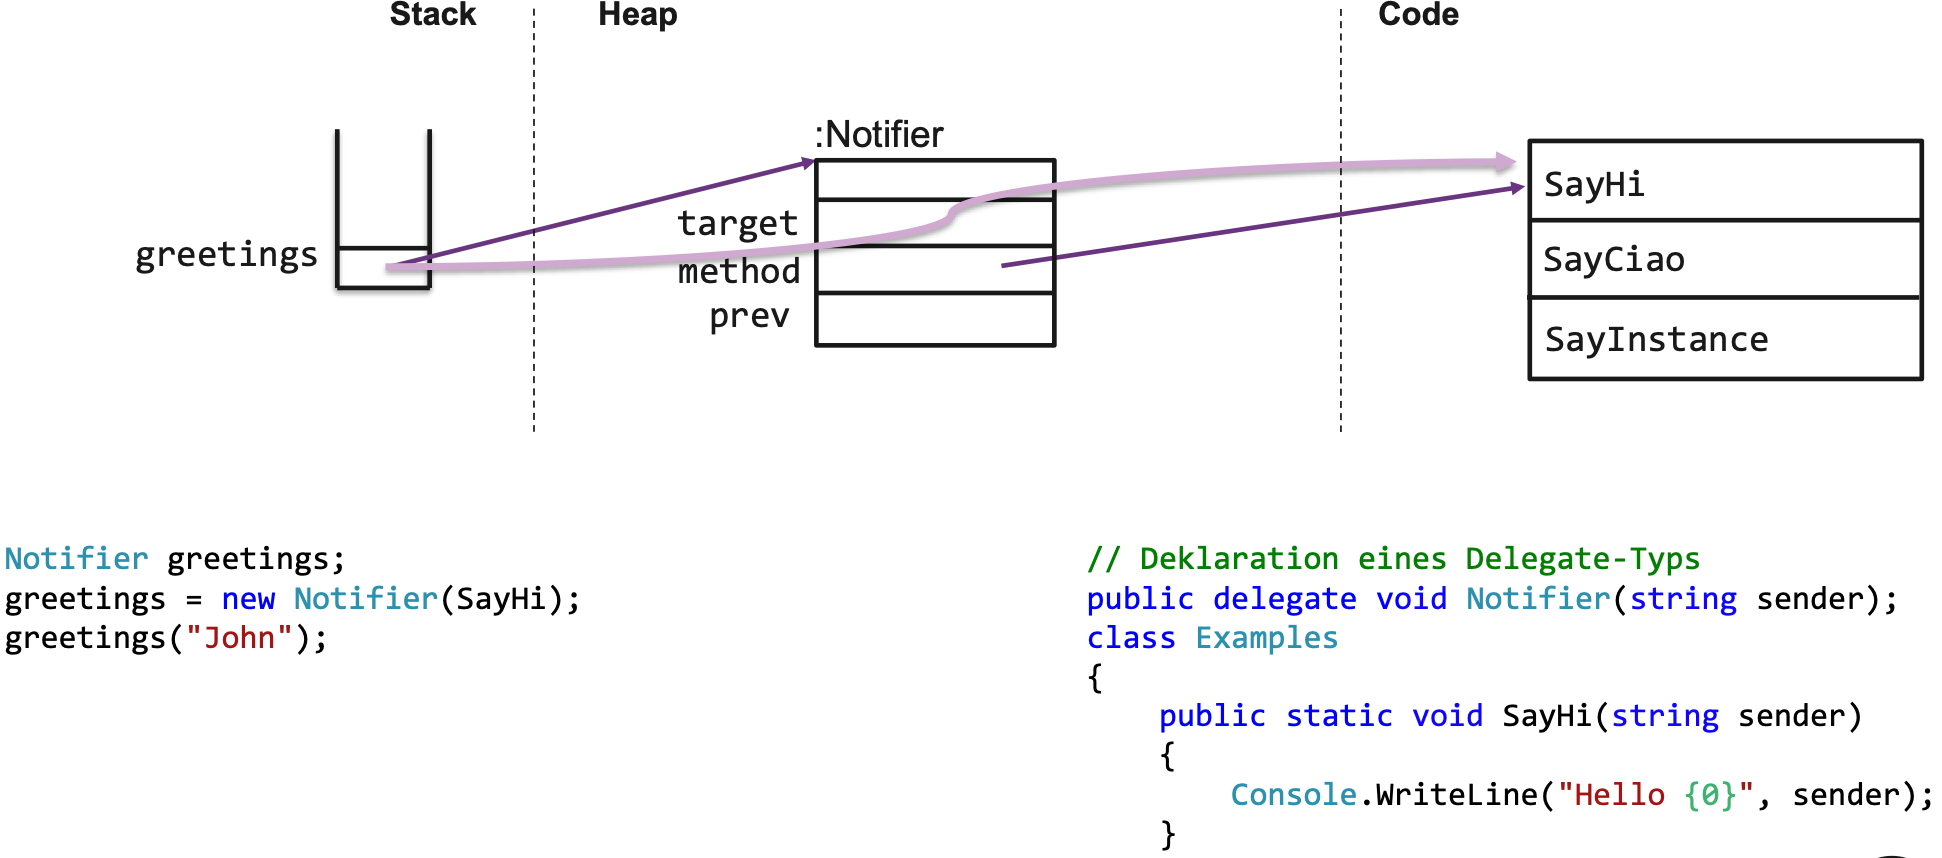
\includegraphics[scale=.26]{graphic/delegate/statisch.png}
\end{center}
\vspace{-8pt}

\subsubsection{Verwendung / Instanz}
\begin{center}
    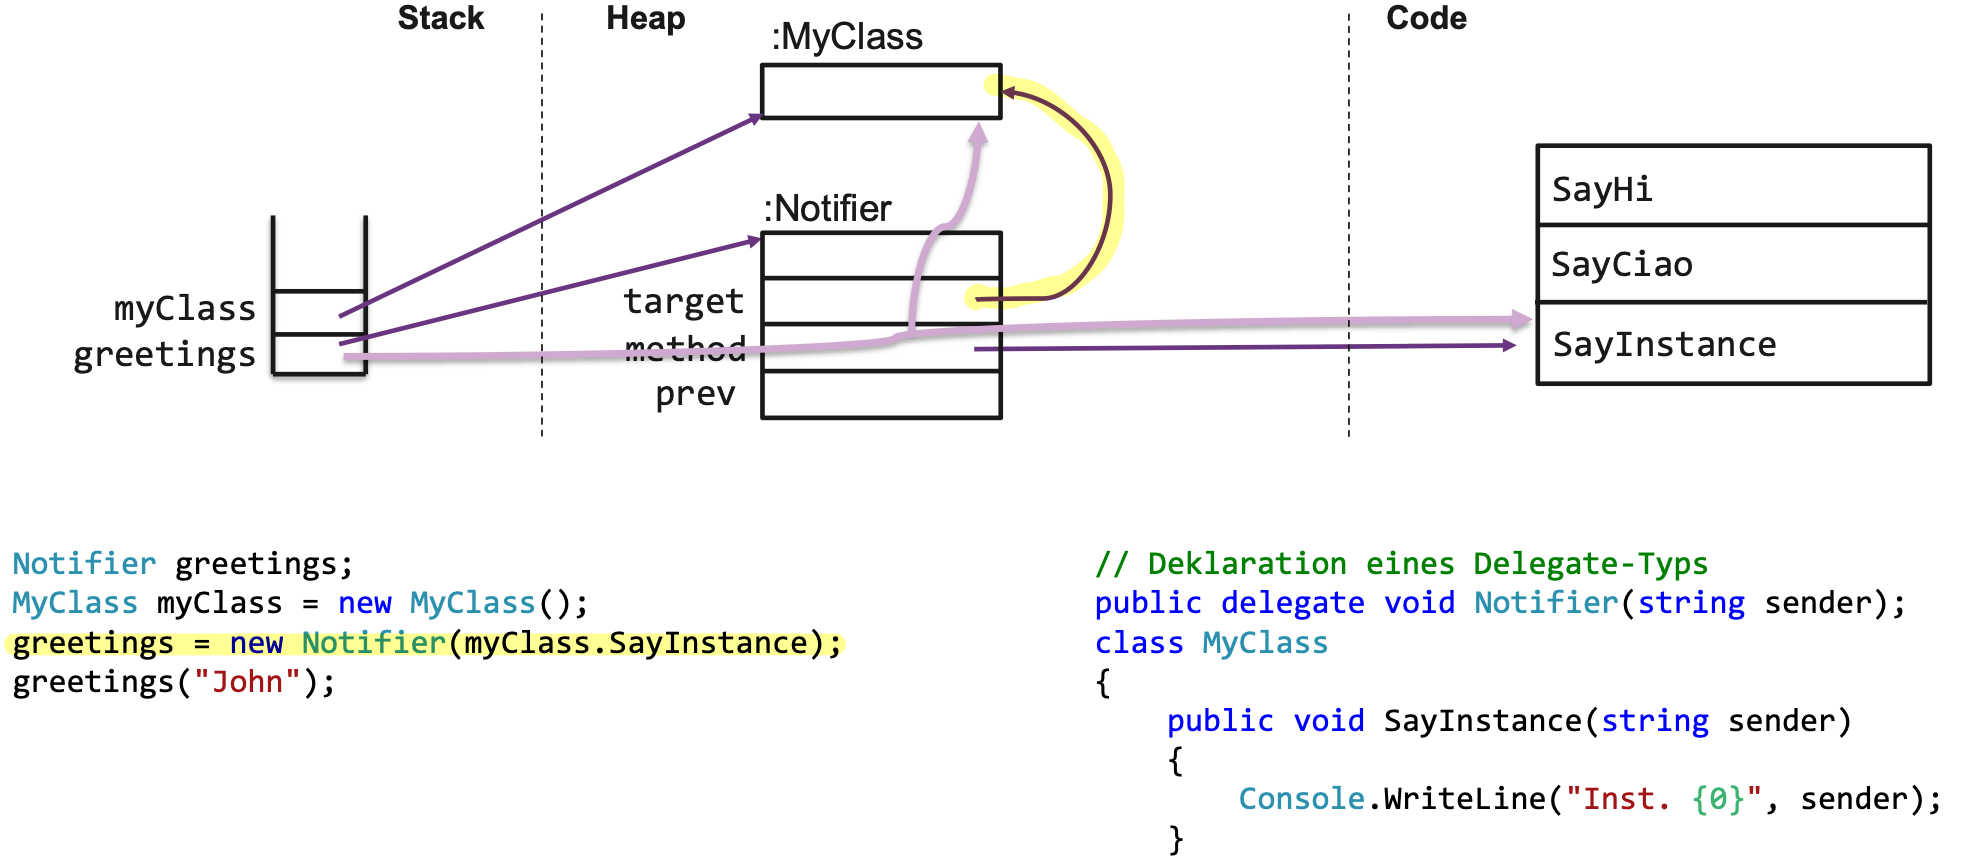
\includegraphics[scale=.26]{graphic/delegate/Instanz.png}
\end{center}
\vspace{-8pt}

\subsubsection{Zuweisung einer Methode}
Zuweisungs-Syntax:
\begin{lstlisting}
DelegateType delegateVar = obj.Method;
\end{lstlisting}

\begin{itemize}
    \item Ein Delegate speichert Methode (Method) und Empfänger-Objekt(obj)
    \item obj kann this bedeuten, deshalb weggelassen werden
    \item Method:
    \begin{itemize}
        \item kann static stein
        \item nicht abstract
        \item darf virtual, override und new sein
        \item muss mit Signatur von DelegateType übereinstimmen
    \end{itemize}
\end{itemize}

\subsubsection{Aufruf einer Delegate-Variable}
Aufruf-Syntax:
\begin{lstlisting}
object result = delegateVar[.Invoke](params);
\end{lstlisting}

\begin{itemize}
    \item Rückgabewert kann weiterverwendet werden falls nicht «void» (z.B. in Variable speichern)
    \item delegateVar darf nicht null sein / muss geprüft werden
    \begin{itemize}
        \item delegateVar?.Invoke(params);
    \end{itemize}
\end{itemize}

\subsection{Multicast Delegates}

\subsubsection{Übersicht}
\begin{itemize}
    \item  Jeder Delegate-Typ ist ein Multicast Delegate
    \item kann beliebig viele Methoden-Referenzen enthalten
    \item Zuweisung mit =
    \item Zuweisung mit +=
    \item Zuweisung mit -=
\end{itemize}
\begin{lstlisting}
public delegate void Notifier(string sender);

class Examples {

    public static void Test() {
        Notifier greetings;
        greetings = SayHi;
        greetings += SayCiao;
        greetings("John");
}

    private static void SayHi(string sender) {
    Console.WriteLine("Hello {0}", sender);}

    private static void SayCiao(string sender) {
    Console.WriteLine("Good bye {0}", sender);}
}
\end{lstlisting}

\subsubsection{Objektmodell}
Implementation in Form einer Linked List
\begin{itemize}
    \item target: Referenz auf Zielobjekt
    \item method: Methoden-Referenz
    \item prev: Referenz auf letztes Delegate
\end{itemize}

\vspace{-8pt}
\begin{center}
    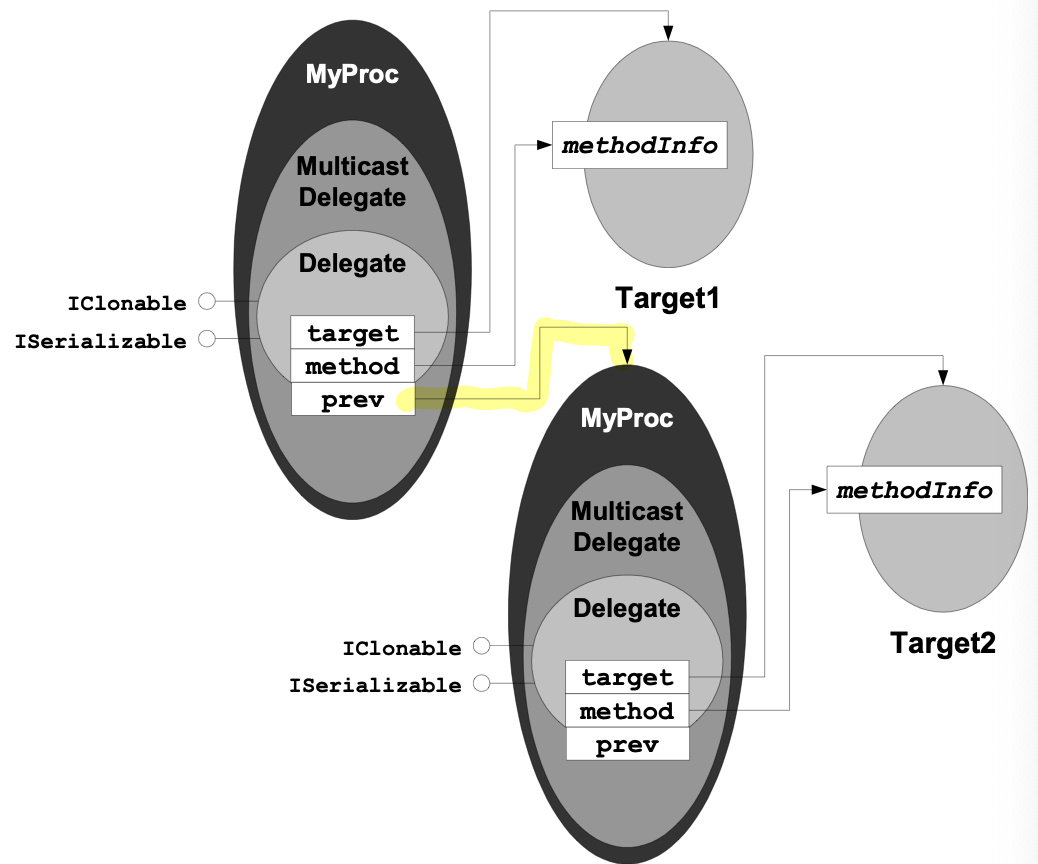
\includegraphics[scale=.34]{graphic/delegate/Objektmodell.png}
\end{center}
\vspace{-8pt}

\subsection{Funktionsparameter}
\begin{itemize}
    \item Methode für das Ausführen einer beliebigen Aktion auf jedem Element eines Arrays
    \item Ansatz: Funktion ForAll
    \begin{itemize}
        \item Int-Array mit Elementen
        \item Delegate mit auszuführender Funktion
    \end{itemize}
    \item Building Blocks
\end{itemize}

\begin{lstlisting}
public delegate void Action(int i);

public class MyClass {

    public static void PrintValues(int i)
    { Console.WriteLine("Value {0}", i); }

    public void SumValues(int i) { Sum += i; }
    public int Sum { get; private set; }
}

public class FunctionParameterTest {

    static void ForAll(int[] array, Action action)
    {
        Console.WriteLine("ForAll called...");
        if (action == null) { return; }
        foreach (int t in array) {
        action(t);
        }
    }
}
\end{lstlisting}

\subsection{Callback}

\subsubsection{Übersicht}

\begin{itemize}
    \item Tickende Uhr
    \begin{itemize}
        \item Benachrichtigung beim Ticken
        \item Subscribe / Unsubscribe Logik
    \end{itemize}
    \item Ansatz
    \begin{itemize}
        \item Clock-Objekt hält Liste von Callbacks
        \item Liste wird beim Ticken benachrichtigt
    \end{itemize}
    \item Implementation
    \begin{itemize}
        \item Interfaces
        \item Delegates
        \item Events
    \end{itemize}
\end{itemize}

\subsubsection{Implementation mit Delegates}
\begin{lstlisting}
public class ClockObserver {
    private string name;
    public ClockObserver(string name) { this.name = name; }

    public void OnTickEvent(int ticks, int i) {
    Console.WriteLine("Observer {0} : Clock mit Interval {2}
    hat zum {1}. Mal getickt.", name, ticks, i);}
}

public delegate void TickEventHandler (int ticks, int interval);
    public class Clock {
        private TickEventHandler OnTickEvent;
        public void add_OnTickEvent(TickEventHandler h) { OnTickEvent += h; }
        public void remove_OnTickEvent(TickEventHandler h) { OnTickEvent -= h; }
        private void Tick(object sender, EventArgs e) {
        ticks++; OnTickEvent?.Invoke(ticks, interval);}
}

public static void Test() {
    Clock c1 = new Clock(1000);
    Clock c2 = new Clock(2000);
    ClockObserver t1 = new ClockObserver("O1");
    ClockObserver t2 = new ClockObserver("O2");

    //Observers anmelden
    c1.add_OnTickEvent(t1.OnTickEvent);
    c2.add_OnTickEvent(t2.OnTickEvent);

    //Observers abmelden
    c1.remove_OnTickEvent(t1.OnTickEvent);
    c2.remove_OnTickEvent(t2.OnTickEvent); }
\end{lstlisting}
	%! Author = mariuszindel
%! Date = 02.11.20

\section{Events}

\subsection{Übersicht}
\begin{itemize}
    \item Reines Compiler-Feature / Syntactic Sugar
\end{itemize}

\subsection{Callback-Tick}
\begin{itemize}
    \item «OnTickEvent» Delegate wird private
    \begin{itemize}
        \item Kann also nur noch intern ausgelöst werden
    \end{itemize}
    \item Subscribe / Unsubscribe Logik wird public generiert
    \item Observer bleibt identisch
\end{itemize}

\begin{lstlisting}
public delegate void TickEventHandler (int ticks, int interval);

public class Clock { £(Notifier/observer)£
    public event TickEventHandler OnTickEvent;

    private void Tick(object sender, EventArgs e) {
    ticks++; OnTickEvent?.Invoke(ticks, interval); }
}
\end{lstlisting}


\subsection{Event Handling im .NET Framework}

Standard-Syntax bei Events:
\begin{lstlisting}
public delegate void AnyHandler(object sender, AnyEventArgs e);
\end{lstlisting}

\begin{itemize}
    \item Rückgabetyp void
    \item 1. Parameter object sender
    \begin{itemize}
        \item Sender des Events
        \item Absender übergibt bei Aufruf des Delegates / Events «this» mit
    \end{itemize}
    \item 2. Parameter AnyEventArgs e
    \begin{itemize}
        \item Beliebige Sub-Klasse von «EventArgs»
        \item Enthält Informationen zum Event
        \item Argumente können jeder ergänzt werden ohne Anpassung der Signatur
    \end{itemize}
\end{itemize}

\subsection{Anonyme Methoden}

\subsubsection{Übersicht}
\begin{itemize}
    \item Methodencode wird in-place angegeben
    \item Keine Deklaration einer Methode nötig
    \item Anonyme Methode kann auf lokale Variable «sum» zugreifen
    \item Return beendet anonyme Methode, nicht die äussere Methode
\end{itemize}
\begin{lstlisting}
class AnonymousMethods {
    void Foo() {
        list.ForEach(delegate(int i)
            { Console.WriteLine(i); }
);

    int sum = 0;
    list.ForEach(delegate(int i)
    { sum += i; });
    }
}
\end{lstlisting}

\subsubsection{Closures / Outer Variables (Äussere Variablen)}
\begin{itemize}
    \item Anonyme Methode greift auf Variable der umgebenden Methode zu
    \item Variable wird in Hilfsobjekt ausgelagert
    \item Hilfsobjekt gleich lange wie Delegate-Objekt
    \item Adder ist eine Closure
\end{itemize}
	%! Author = mariuszindel
%! Date = 02.11.20

\section{Generics}

\subsection{Überblick}
\begin{itemize}
    \item Ohne Festlegung auf einen fixen Typen
    \begin{itemize}
        \item Erlaubt die Implementation von Strukturen ohne Verwendung von «Object»
        \item Anstelle von «Object» wird «T» verwendet
    \end{itemize}
    \item Vorteile
    \begin{itemize}
        \item Hohe Wiederverwendbarkeit
        \item Typsicherheit
        \item Performance
    \end{itemize}
    \item Boxing / Typumwandlungen fallen weg
    \item  kann generisch sein:
    \begin{itemize}
        \item Klasse / Struct / Interface / Delegates / Events
        \item Methoden
    \end{itemize}
\end{itemize}

\subsubsection{Laufzeiteffizienz}
\begin{center}
    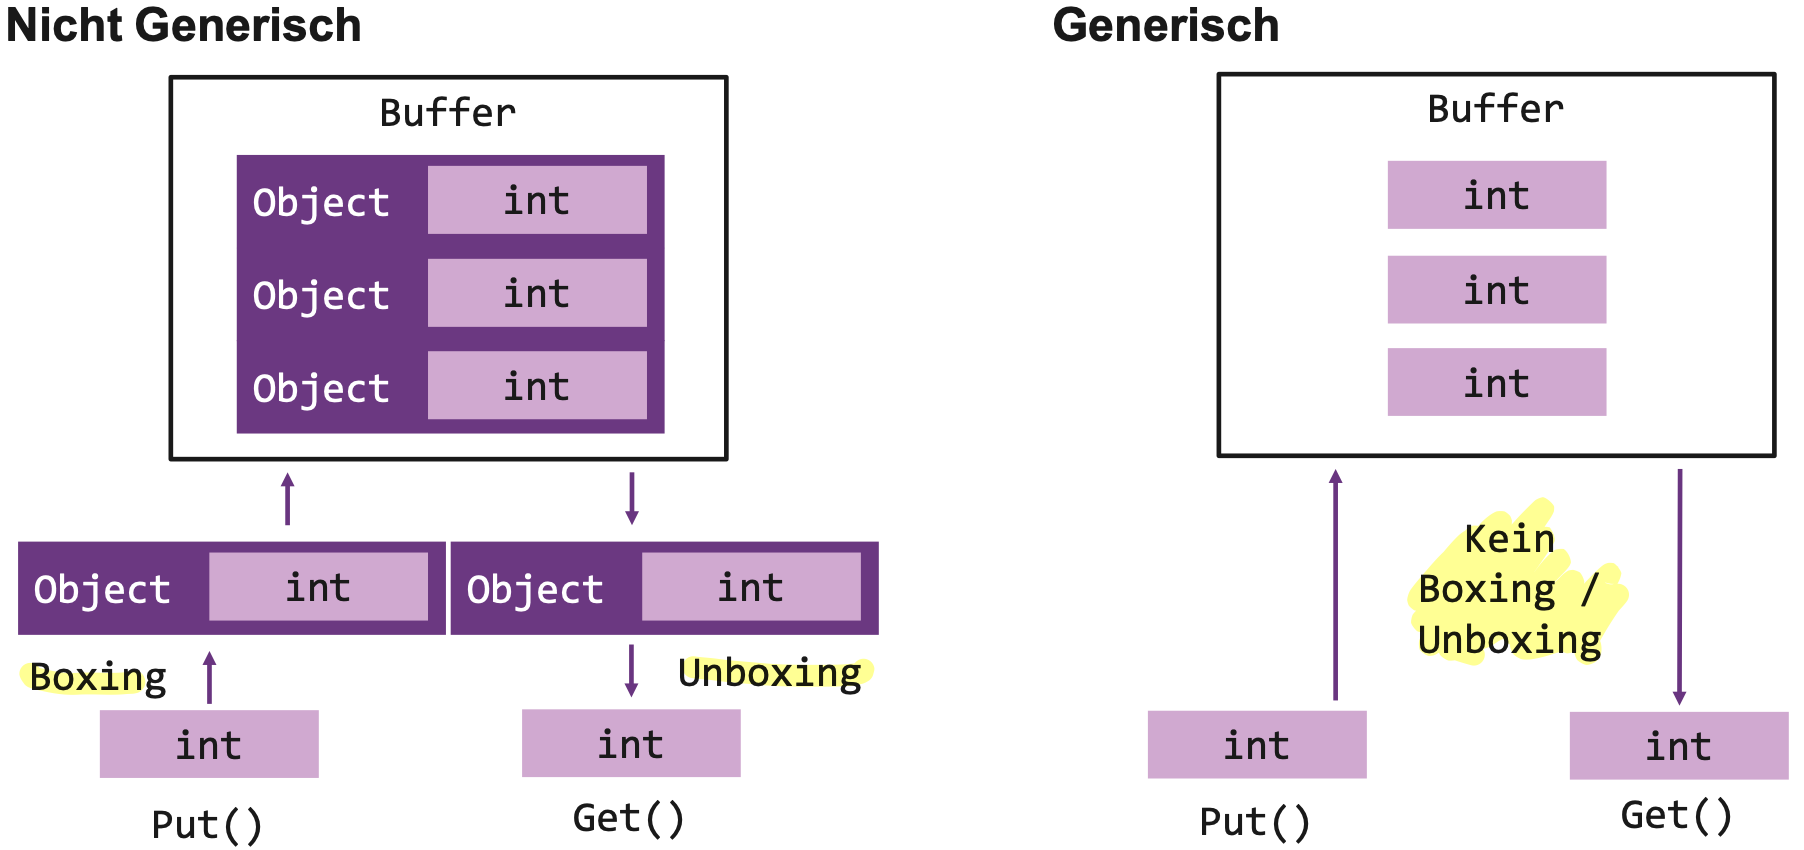
\includegraphics[scale=.25]{graphic/generics/Laufzeiteffizienz.png}
\end{center}
\vspace{-8pt}


\subsection{Type Constraints}
\begin{itemize}
    \item Mit Type Constraint «where TPriority : IComparable»
    \begin{itemize}
        \item Alle Members von «Object»
        \item Alle Members von «IComparable»
    \end{itemize}
\end{itemize}
\begin{lstlisting}
class OrderedBuffer<TElement, TPriority>
    where TPriority : IComparable
{ ... }
\end{lstlisting}

\vspace{-8pt}
\begin{center}
    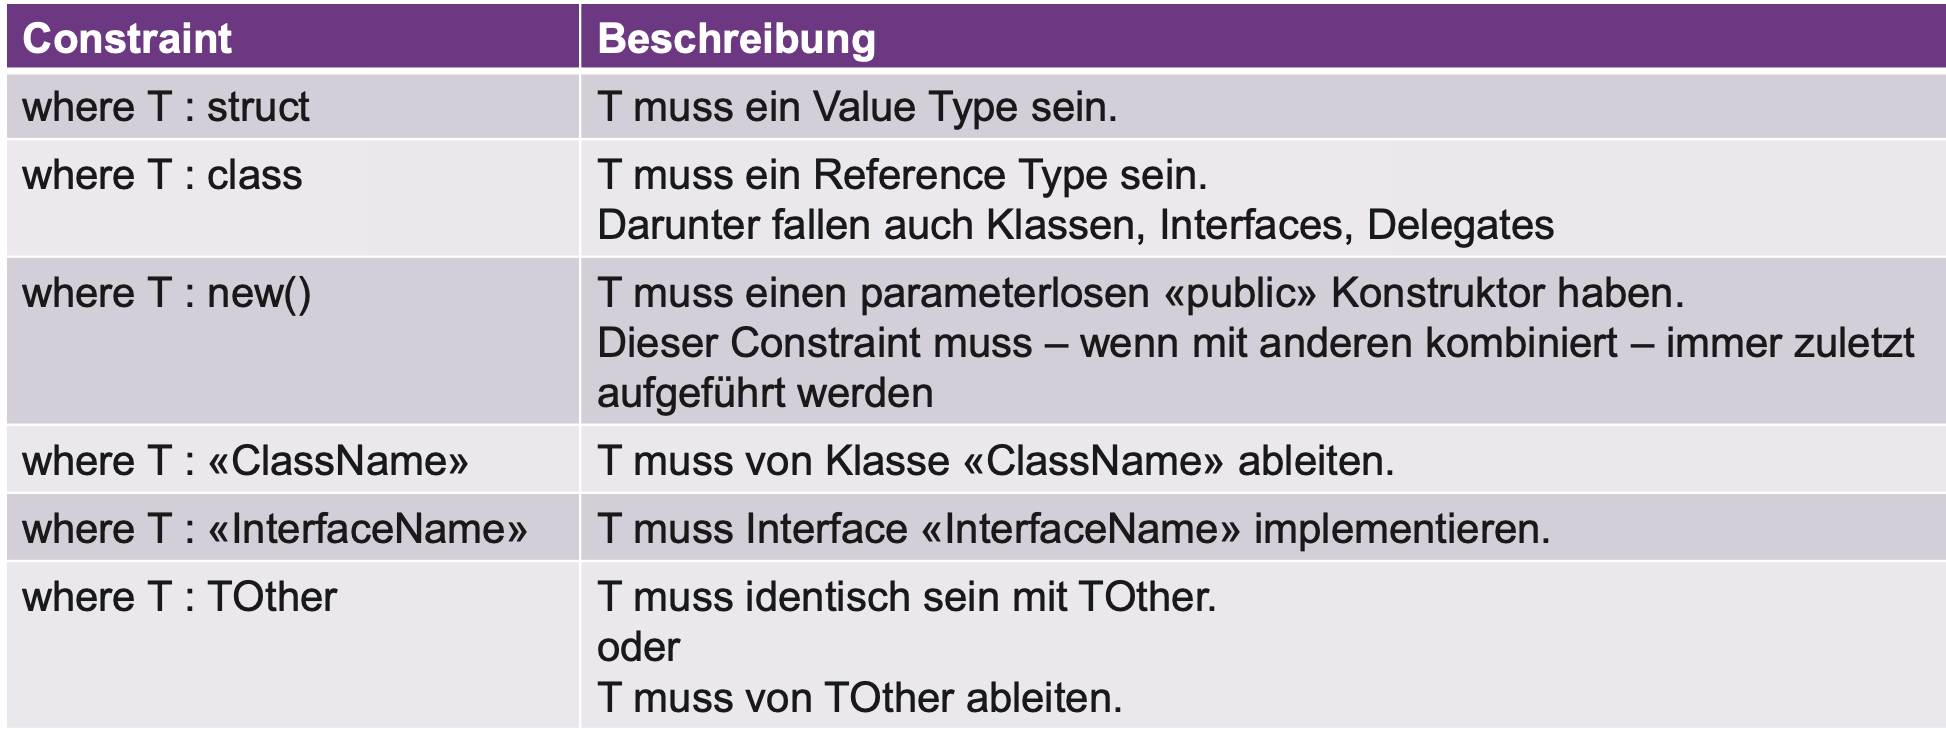
\includegraphics[scale=.23]{graphic/generics/Type Constraints.png}
\end{center}
\vspace{-8pt}

\subsubsection{T : struct}
\begin{itemize}
    \item T muss ein Value Type sein
    \item Implikationen
    \begin{itemize}
        \item T liegt auf dem Stack oder inline in einem Objekt
        \item T ist nie «null»
    \end{itemize}
\end{itemize}
\begin{lstlisting}
public void Work<T>(T source)
where T : struct
{ ... }
\end{lstlisting}

\subsubsection{T : class}
\begin{itemize}
    \item T muss ein Reference Type sein
    \item Implikationen
    \begin{itemize}
        \item T liegt auf dem Heap
        \item T kann «null» sein
    \end{itemize}
\end{itemize}
\begin{lstlisting}
public void Work<T>(T source)
where T : class
{ ... }
\end{lstlisting}

\subsubsection{T : new()}
\begin{itemize}
    \item T muss einen parameterlosen «public» Konstruktor haben
    \item Implikationen
    \begin{itemize}
        \item  T kann instanziert werden
    \end{itemize}
\end{itemize}
\begin{lstlisting}
public T GetInstance<T>()
    where T : new() {
    return new T();
}
\end{lstlisting}

\subsubsection{T : ClassName}
\begin{itemize}
    \item T muss von Klasse «ClassName» ableiten
    \item Implikationen
    \begin{itemize}
        \item T bietet alle Members von «ClassName»
    \end{itemize}
\end{itemize}
\begin{lstlisting}
public void Work<T>(T source)
where T : List<int>
{ ... }
\end{lstlisting}

\subsubsection{T : InterfaceName}
\begin{itemize}
    \item T muss Interface «InterfaceName» implementieren
    \item Implikationen
    \begin{itemize}
        \item T bietet alle Members von «InterfaceName»
    \end{itemize}
\end{itemize}
\begin{lstlisting}
public void FillList<T>(T source)
    where T : IList<int>, IEnumerable<int>
{ ... }
\end{lstlisting}

\subsubsection{T : TBase}
\begin{itemize}
    \item T muss identisch sein mit TBase oder T muss von TBase ableiten
\end{itemize}
\begin{lstlisting}

\end{lstlisting}
public void Work<T, TBase>(T a, TBase b)
where T : TBase {
    T t1 = a;
    T t2 = b; // Compilerfehler
    TBase to1 = a;
    TBase to2 = b;
}


\subsection{Vererbung}

Generische Klassen können von anderen generischen Klassen erben

\begin{itemize}
    \item Normale Klassen\\
    class MyList<T> : List { }
    \item Weitergabe des Typparameters an generische Basisklasse\\
    class MyList<T> : List<T> { }
    \item Konkretisierte generische Basisklasse\\
    class MyIntList : List<int> {}
    \item Mischform \\
    class MyIntKeyDict<T> : Dictionary<int, T> { }
    \item Typparameter werden nicht vererbt
    class MyList : List<T> { } // Compilerfehler
\end{itemize}


\subsection{Nullable Types}

\begin{itemize}
    \item «default(T)»
    \begin{itemize}
        \item Reference Types: null
        \item Value Types: 0, false oder \textbackslash0
    \end{itemize}
\end{itemize}

\begin{lstlisting}
public void NullExamples<T>() {
// Nullwerte zuweisen 
    T x1 = null;       // Compilerfehler
    T x2 = 0;          // Compilerfehler 
    T x3 = default(T); // OK
    T x4 = default;    // OK (C# 7.1)
}
\end{lstlisting}

\subsubsection{Struct «Nullable»}
\begin{center}
    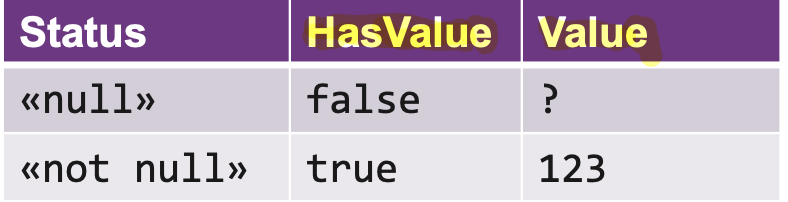
\includegraphics[scale=.3]{graphic/generics/Struct Nullable.png}
\end{center}
\begin{lstlisting}
public struct Nullable<T> where T : struct
{
    public Nullable(T value);

    public bool HasValue { get; }
    public T Value { get; }
}
\end{lstlisting}

\subsubsection{T? Syntax}
\begin{lstlisting}
int? x = null; 
double? y = null;
\end{lstlisting}


\subsubsection{Sicheres lesen \& Type Cast}
\begin{lstlisting}
// Klassisch
int x1 = x.HasValue ? x.Value: default;

// Via Methode
int x2 = x.GetValueOrDefault();

// Via Methode inkl. eigenem Default
int x3 = x.GetValueOrDefault(-1);

// Definition
private int? GetNullableInt() {
return null;
}
\end{lstlisting}


\subsubsection{?? Und ??= Operator \& Casts}

\begin{lstlisting}
// wenn i null -> -1
int i = GetNullableInt() ?? -1;

int? i = null;
i ??= 1234; // i = i ?? 1234;

\end{lstlisting}


\subsection{Generische Collections}
\begin{center}
    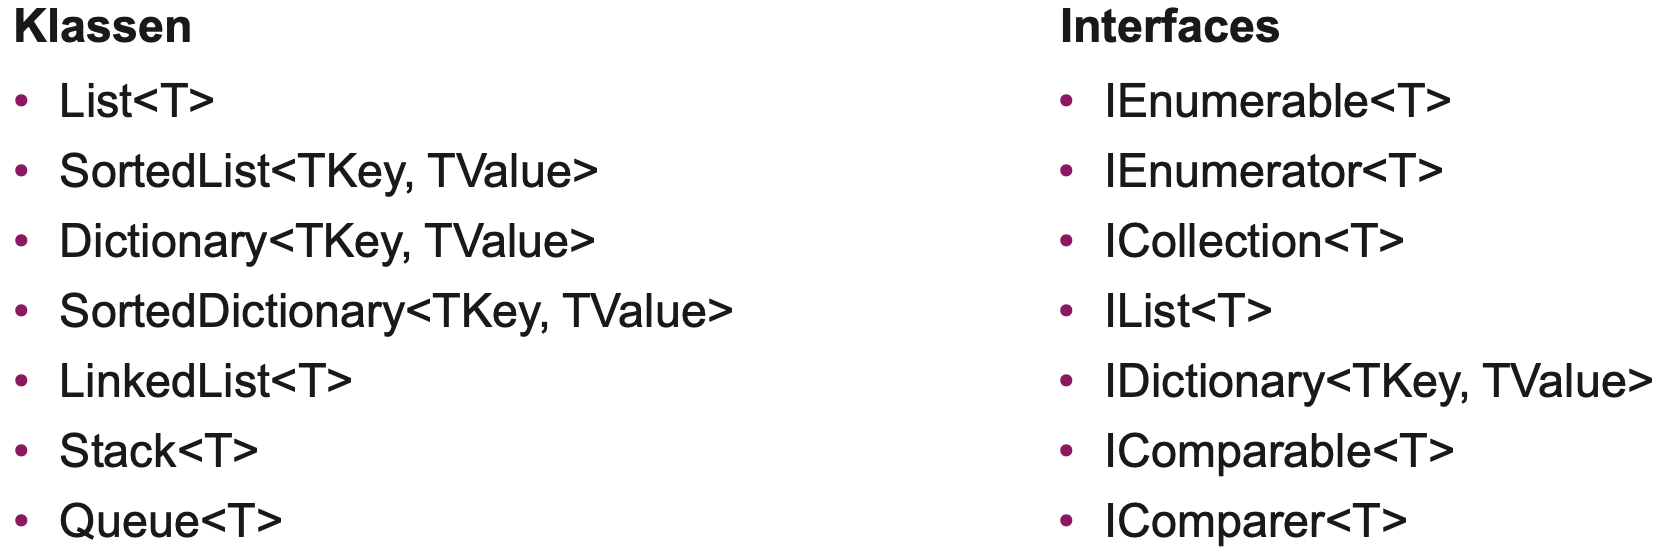
\includegraphics[scale=.24]{graphic/generics/Generische Listentypen.png}
    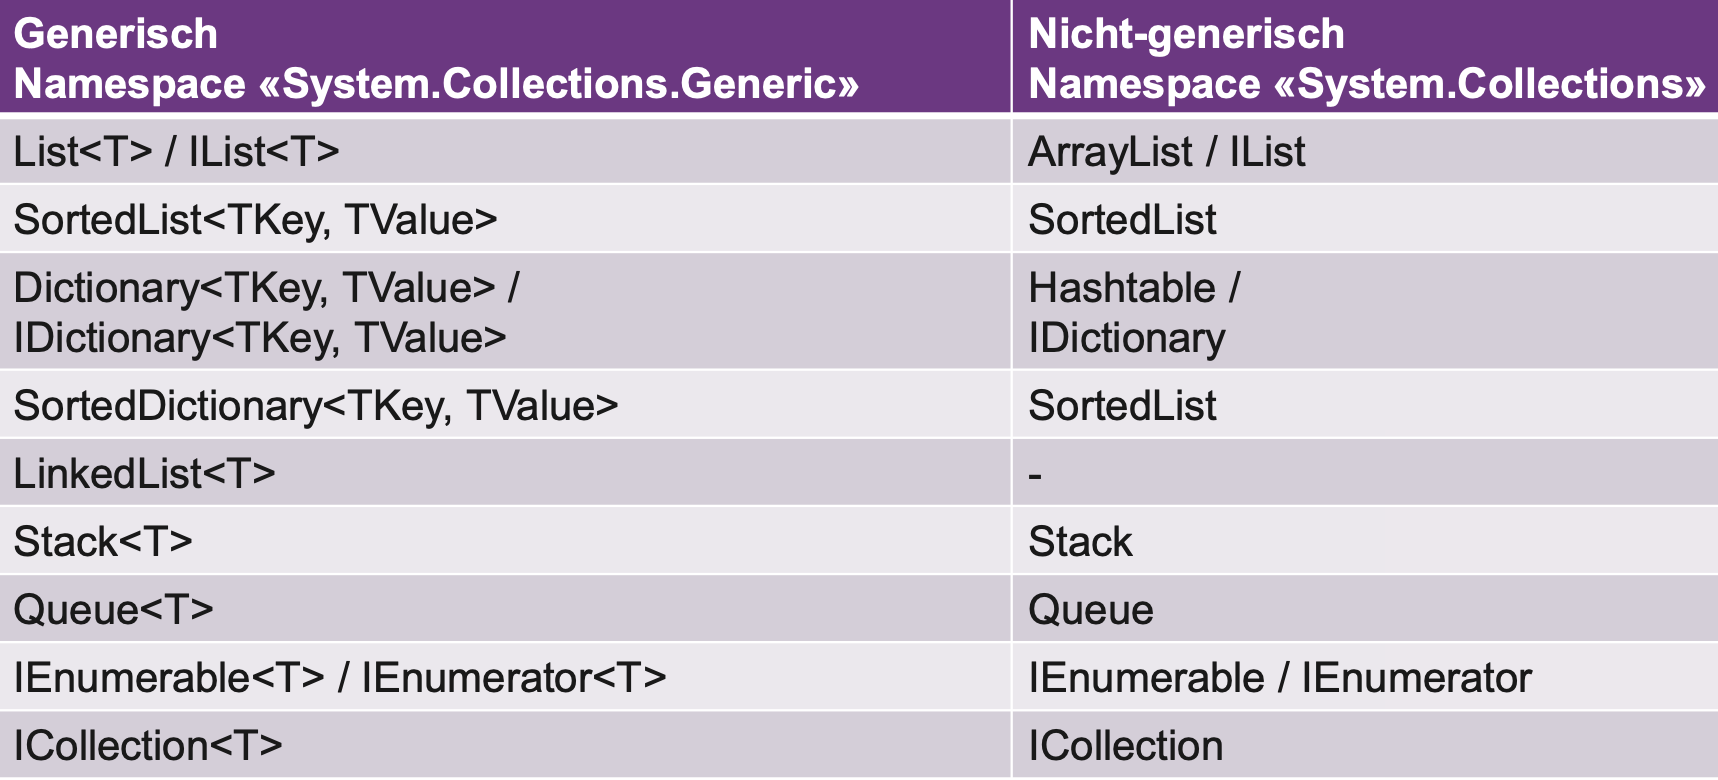
\includegraphics[scale=.24]{graphic/generics/Nicht-generische Pendants.png}
\end{center}

\newpage
	%! Author = mariuszindel
%! Date = 02.11.20

\section{Iteratoren}

\subsection{foreach-Loop}
\subsubsection{Übersicht}
\begin{itemize}
    \item Wird für das Iterieren über Collections verwendet
    \item Jumps
    \begin{itemize}
        \item continue $\rightarrow$ unterbricht aktuelle Iteration
        \item break $\rightarrow$ unterbricht gesammten Loop
    \end{itemize}
\end{itemize}
\subsubsection{Syntax}
Kriterien für «collection»:
\begin{itemize}
    \item Muss IEnumerable / IEnumerable<T> implementieren
    \item Muss einer Implementation von IEnumerable / IEnumerable<T> «ähneln»
    \begin{itemize}
        \item «collection» hat Methode GetEnumerator() mit Rückgabewert «e»
        \item «e» hat eine Methode MoveNext() mit Rückgabewert «bool»
        \item «e» hat ein Property «Current»
    \end{itemize}
\end{itemize}
\begin{lstlisting}
int[] list = new int[] { 1, 2, 3, 4, 5, 6 };
foreach (int i in list) {
    if (i == 3) continue;
    if (i == 5) break;
    Console.WriteLine(i);
}
\end{lstlisting}

\subsubsection{Sequenzdiagramm}
\begin{center}
    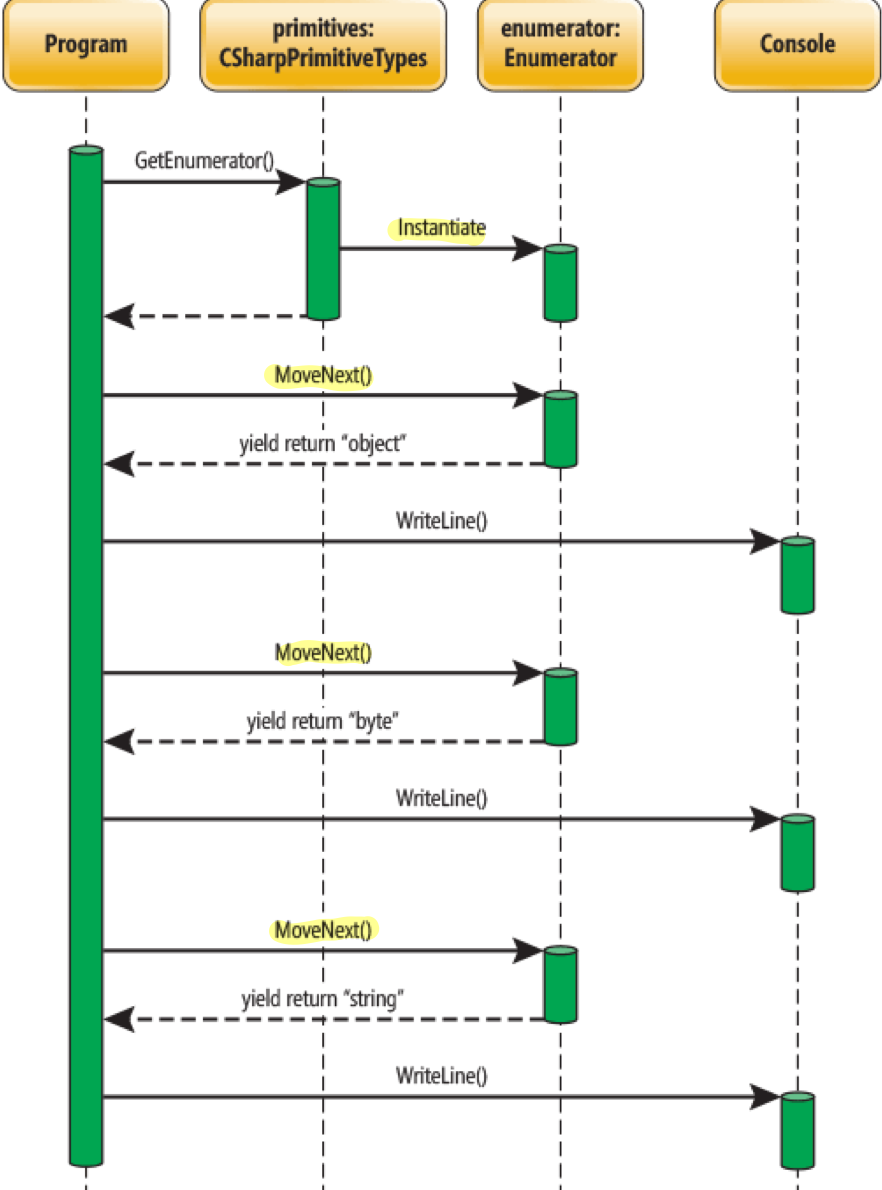
\includegraphics[scale=.33]{graphic/iterator/Sequenzdiagramm.png}
\end{center}


\subsection{Iteratoren}
\subsubsection{Interfaces}
Iterator = Enumerator!

\begin{itemize}
    \item Interface IEnumerable
\end{itemize}
\begin{lstlisting}
public interface IEnumerable {
    IEnumerator GetEnumerator();
}
\end{lstlisting}

\begin{itemize}
    \item Interface IEnumerator
\end{itemize}
\begin{lstlisting}
public interface IEnumerator {
    object Current { get; }
    bool MoveNext();
    void Reset();
}
\end{lstlisting}

\begin{itemize}
    \item Interface IEnumerable<T>
\end{itemize}
\begin{lstlisting}
public interface IEnumerable<out T>
    : IEnumerable {
    IEnumerator<T> GetEnumerator();
}
\end{lstlisting}

\begin{itemize}
    \item Interface IEnumerator<T>
\end{itemize}
\begin{lstlisting}
public interface IEnumerator<out T>
    : IDisposable, IEnumerator {
    T Current { get; }
    // Weitere Members werden vererbt
}
\end{lstlisting}


\subsubsection{Zugriff}
\begin{itemize}
    \item Mehrere aktive Iteratoren zur gleichen Zeit erlaubt
    \item Enumerator-Objekt muss Zustand vollständig kapseln
    \item Collection darf während Iteration nicht verändert werden
\end{itemize}


\subsubsection{Implementationsbeispiel (nicht-generisch)}
\begin{itemize}
    \item Klasse «MyList» als IEnumerable
    \item Klasse «MyEnumerator» als IEnumerator
\end{itemize}
\begin{lstlisting}
class MyList : IEnumerable {
    public IEnumerator GetEnumerator()
        { return new MyEnumerator(); }

    class MyEnumerator : IEnumerator {
    {

        public object Current }
            { get { /* ... */ } }

        public bool MoveNext() { /* ... */ }
        public void Reset() { /* ... */ }
    }
}
\end{lstlisting}

\subsubsection{Implementationsbeispiel (generisch)}
\begin{itemize}
    \item Klasse «MyList» als IEnumerable<T>
    \item Klasse «MyEnumerator» als IEnumerator<T>
\end{itemize}
\begin{lstlisting}
class MyIntList : IEnumerable<int> {

    public IEnumerator<int> GetEnumerator()
        { return new MyIntEnumerator(); }

    IEnumerator IEnumerable.GetEnumerator()
        { return GetEnumerator(); }

    class MyIntEnumerator : IEnumerator<int> {

        public int Current
            { get { /* ... */ } }
        object IEnumerator.Current
            { get { /* ... */ } }

        public bool MoveNext() { /* ... */ }
        public void Reset() { /* ... */ }
        public void Dispose() { /* ... */ }
    }
}
\end{lstlisting}

\subsection{Iterator-Methoden}
\subsubsection{Syntax}
Beinhaltet mindestens ein «yield return» Statement!
\begin{itemize}
    \item Gibt den nächsten Wert für die nächste Iteration eines «foreach» Loops zurück
    \item Syntax:\\
    yield return «expr»;
    \item «yield break» Statement terminiert die Iteration

\end{itemize}
\subsubsection{Implementationsbeispiel}
\begin{lstlisting}
class MyIntList {
    public IEnumerator<int> GetEnumerator() {
        yield return 1;
        yield return 3;
        yield break;
        yield return 6;
    }}
\end{lstlisting}

\subsection{Spezifische Iteratoren}
\subsubsection{Standard Iterator-Methode}
Iterator:
\begin{lstlisting}
class MyIntList {
    private int[] data = new int[10];

    // Standard Iterator
    public IEnumerator<int> GetEnumerator() {
        for (int i = 0; i < data.Length; i++)
        yield return data[i];
}}
\end{lstlisting}

Anwendung:
\begin{lstlisting}
MyIntList list = new MyIntList();
foreach (int elem in list) {
/* ... */ }
\end{lstlisting}


\subsubsection{Spezifische Iterator-Methode}
Iterator:
\begin{lstlisting}
class MyIntList {
    private int[] data = new int[10];

    // Spezifische Iterator-Methode
    public IEnumerable<int> Range(int from, int to) {
        for (int i = from; i < to; i++)
        yield return data[i];
}}
\end{lstlisting}

Anwendung:
\begin{lstlisting}
MyIntList list = new MyIntList();
foreach (int elem in list.Range(2, 7)) {
/* ... */
}
\end{lstlisting}


\subsubsection{Spezifisches Iterator-Property}
Iterator:
\begin{lstlisting}
class MyIntList {
    private int[] data = new int[10];

    // Spezifisches Iterator-Property
    public IEnumerable<int> Reverse {
        get {
            for (int i = data.Length - 1; i >= 0; i--)
                yield return data[i];
}}}
\end{lstlisting}

Anwendung:
\begin{lstlisting}
MyIntList list = new MyIntList();
foreach (int elem in list.Reverse) {
/* ... */
}
\end{lstlisting}

\subsection{Erweiterungsmethoden}
\subsubsection{Übersicht}
\begin{itemize}
    \item Erlaubt das Erweitern bestehender Klassen
    \item Signatur der Klasse wird nicht verändert
    \item Aufruf sieht jedoch so aus, als wäre es eine Methode auf der Klasse
    \item Muss in statischer Klasse deklariert sein
    \item Muss «static» sein
    \item «this» Schlüsselwort voranstehend
\end{itemize}

\subsubsection{Regeln}
\begin{itemize}
    \item Kein Zugriff auf interne Members aus Extension Methode
    \item «ToStringSafe» ist nur sichtbar, wenn der Namespace von «ExtensionMethods» importiert wurde
    \item Bei Konflikt mit Methode auf der Zielklasse gewinnt immer die eigene Methode
    \item Erlaubt auf Klassen / Structs / Interfaces / Delegates / Enumeratoren / Arrays
\end{itemize}
\begin{lstlisting}
public static class ExtensionMethods {
    static string ToStringSafe(this object obj) {
        return obj == null ? string.Empty : obj.ToString();
    }
    public static void Test() {
        int myInt = 0;
        object myObj = new object(); // Objects not null
        myInt.ToString();
        myInt.ToStringSafe();
        myObj.ToString();
        myObj.ToStringSafe(); // Object is null
        myObj = null;
        myObj.ToString(); // Error
        myObj.ToStringSafe(); // Works
}}
\end{lstlisting}

\subsection{Deferred Evaluation}
\subsubsection{Übersicht}
\begin{itemize}
    \item Aufruf von GetEnumerator() oder von Range(…) führt Iterator-Methode noch NICHT aus
    \item Erst der Aufruf von IEnumerator<T>.MoveNext()
    \item $\rightarrow$ Dies passiert implizit im «foreach» Loop
\end{itemize}
\subsubsection{Beispiel}

\subsubsection{Extension Methods und Iteratoren}
\begin{lstlisting}
public class Extensions
{
public static void ForeachIfGreaterThan11(IList<int> source, Action<int> action){
foreach (int elem in source)
{
    if (elem > 10) { action(elem); }
}}}

//neu zu:
public static class Extensions
{
    public static void ForeachIf<T>(
        this IEnumerable<T> source,
        Action<T> action,
        Predicate<T> predicate)
    {
        foreach (T elem in source)
        {
            if (predicate(elem)) {
                action(elem);
        } } }}
\end{lstlisting}

\subsubsection{Grafisch}
\begin{center}
    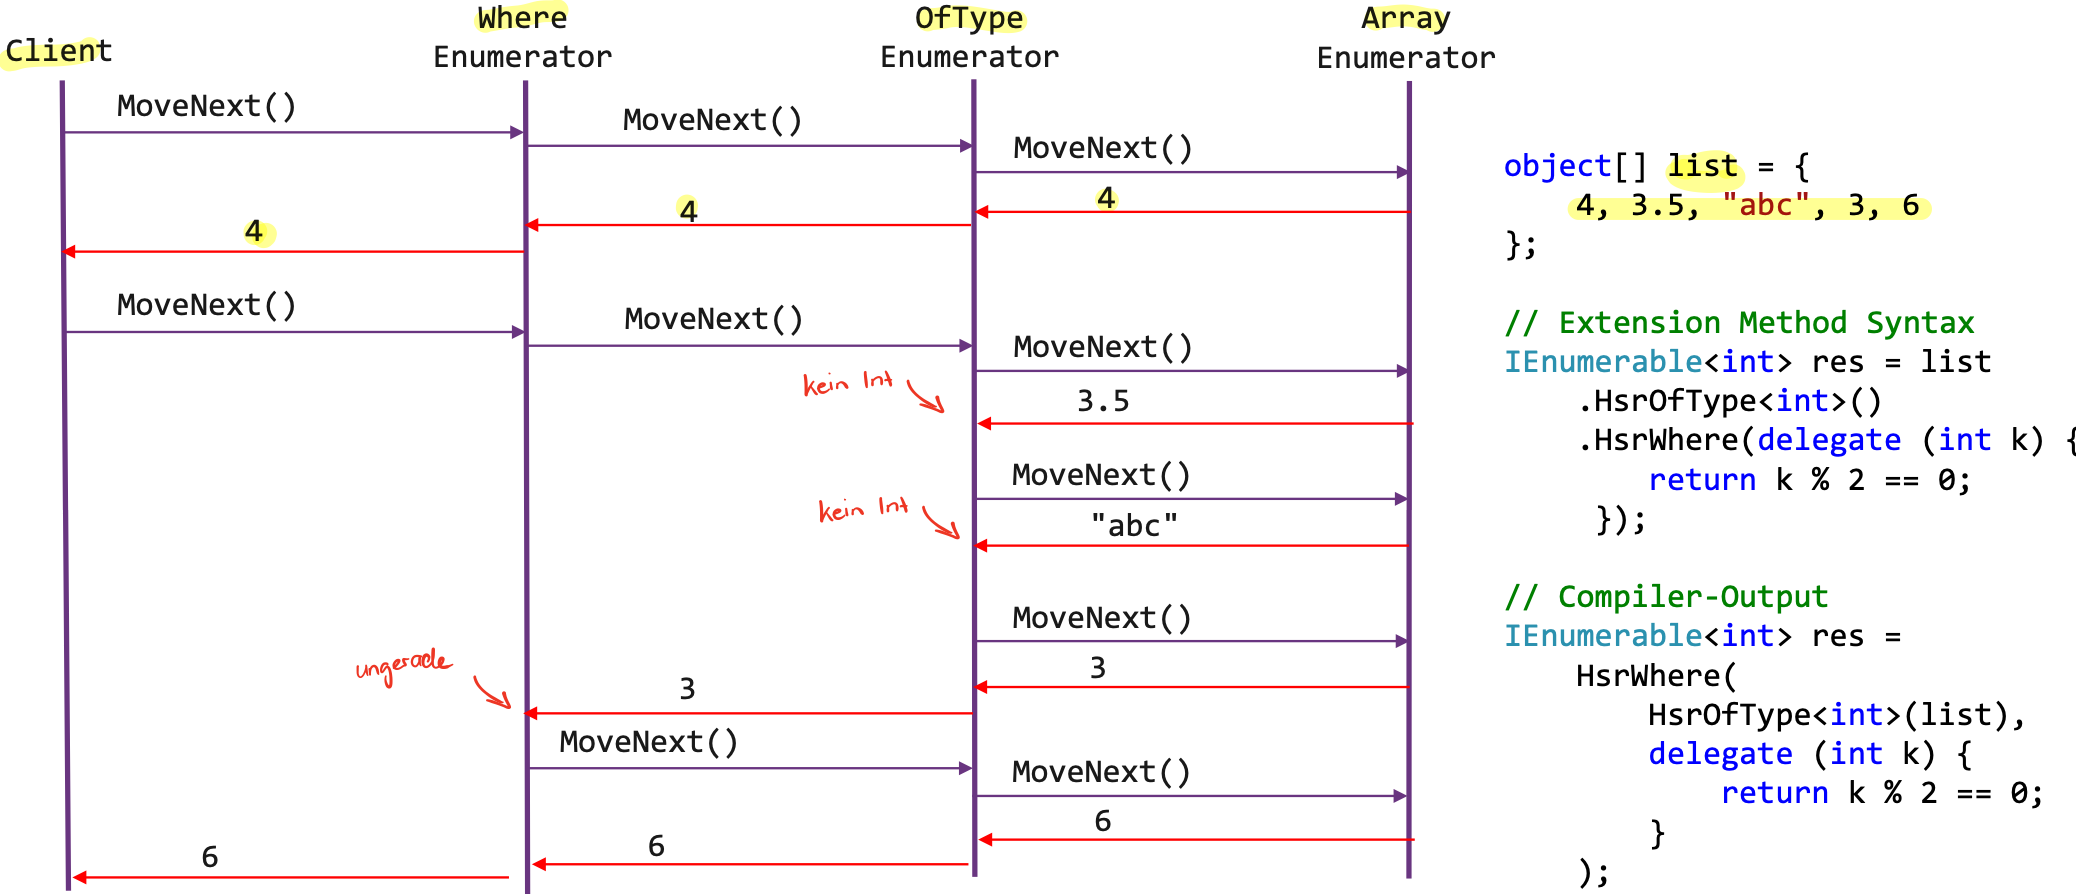
\includegraphics[scale=.24]{graphic/iterator/Deferred Evaluation.png}
\end{center}


\newpage


	%! Author = mariuszindel
%! Date = 02.11.20

\section{Exceptions}

\subsection{Überblick}
\begin{itemize}
    \item Behandelt unerwartete Programmstati oder Ausnahmeverhalten zur Laufzeit
    \item Best Practices
    \begin{itemize}
        \item Exception sind «Ausnahmen»
        \item Wenn möglich Vorbedingungen prüfen um Exceptions zu vermeiden
        \item Exceptions sind «Fehlercodes» vorzuziehen
        \item Konkrete Fehlerbeschreibung $\rightarrow$ konkrete Exception-Klassen verwenden
        \item .NET Exception-Typen verwenden, wenn zutreffend
        \item Aufräumen bei Exceptions (Sockets, File Handles, offene Transaktionen, etc.)
    \end{itemize}
\end{itemize}

\subsection{Syntax}
Basiert auf den Schlüsselwörtern:
\begin{itemize}
    \item try
    \begin{itemize}
        \item Anweisungsblock welcher potenziell eine Ausnahme verursacht
    \end{itemize}
    \item catch
    \begin{itemize}
        \item Anweisungsblock der eine spezielle Ausnahme behandelt
    \end{itemize}
    \item finally
    \begin{itemize}
        \item Anweisungsblock, der nach einem try. sowie auch nach einem catch-Block garantiert einmal ausgeführt wird
    \end{itemize}
    \item throw
    \begin{itemize}
        \item Statement löst eine beliebige Exception aus
    \end{itemize}
\end{itemize}

\begin{lstlisting}
FileStream s = null;
try {
    s = new FileStream(@"C:\Temp\Test.txt",FileMode.Open);
}
catch (FileNotFoundException e) {
    Console.WriteLine("{0} not found", e.FileName);
}
catch (IOException) {
    Console.WriteLine("IO exception occurred");
}
catch {
    Console.WriteLine("Unknown error occurred");
}
finally {
    if (s != null) s.Close();
}
\end{lstlisting}

\subsection{Klasse System.Exception}
\begin{itemize}
    \item Basisklasse für alle Exceptions
    \item Konstruktoren
    \begin{itemize}
        \item mit Fehlerberschreibung und optionaler InnerException
    \end{itemize}
    \item Properties
    \begin{itemize}
        \item InnerException: Verschachtelte Exception
        \item Message: Fehlermeldung als String
        \item Source: Name der Applikation, des Objekts, des Frameworks, etc. welche(s) den Fehler verursarchte
        \item StackTrace: Methodenaufrufkette als String
        \item TargetSite: Ausgeführter Code-Teil der Fehler verursacht
    \end{itemize}
    \item Methoden:
    \begin{itemize}
        \item ToString(): Fehlermeldung und Stack Trace als String
    \end{itemize}
\end{itemize}
\begin{lstlisting}
public class Exception : ISerializable, _Exception {
    public Exception();
    public Exception(string message);
    public Exception(string message, Exception innerException);

    public Exception InnerException { get; }
    public virtual string Message { get; }
    public virtual string Source { get; set; }
    public virtual string StackTrace { get; }
    public MethodBase TargetSite { get; }

    public override string ToString();
/* ... */
}
\end{lstlisting}

\subsubsection{throw}
«throw» Anweisung (explizit)
\begin{lstlisting}
throw new Exception("An error occured");
\end{lstlisting}

\subsubsection{catch-throw}
Klassisch mit «throw e» $\rightarrow$ beginnt einen neuen Stack Trace
\begin{lstlisting}
try {
    throw new Exception("Failure");
}
catch (Exception e) {
throw e; }
\end{lstlisting}

Rethrowing mit «throw» $\rightarrow$ Stack Trace bleibt erhalten
\begin{lstlisting}
try {
    throw new Exception("Failure");
}
catch (Exception e) {
throw; }
\end{lstlisting}

\subsubsection{Exception-Typen}
\begin{center}
    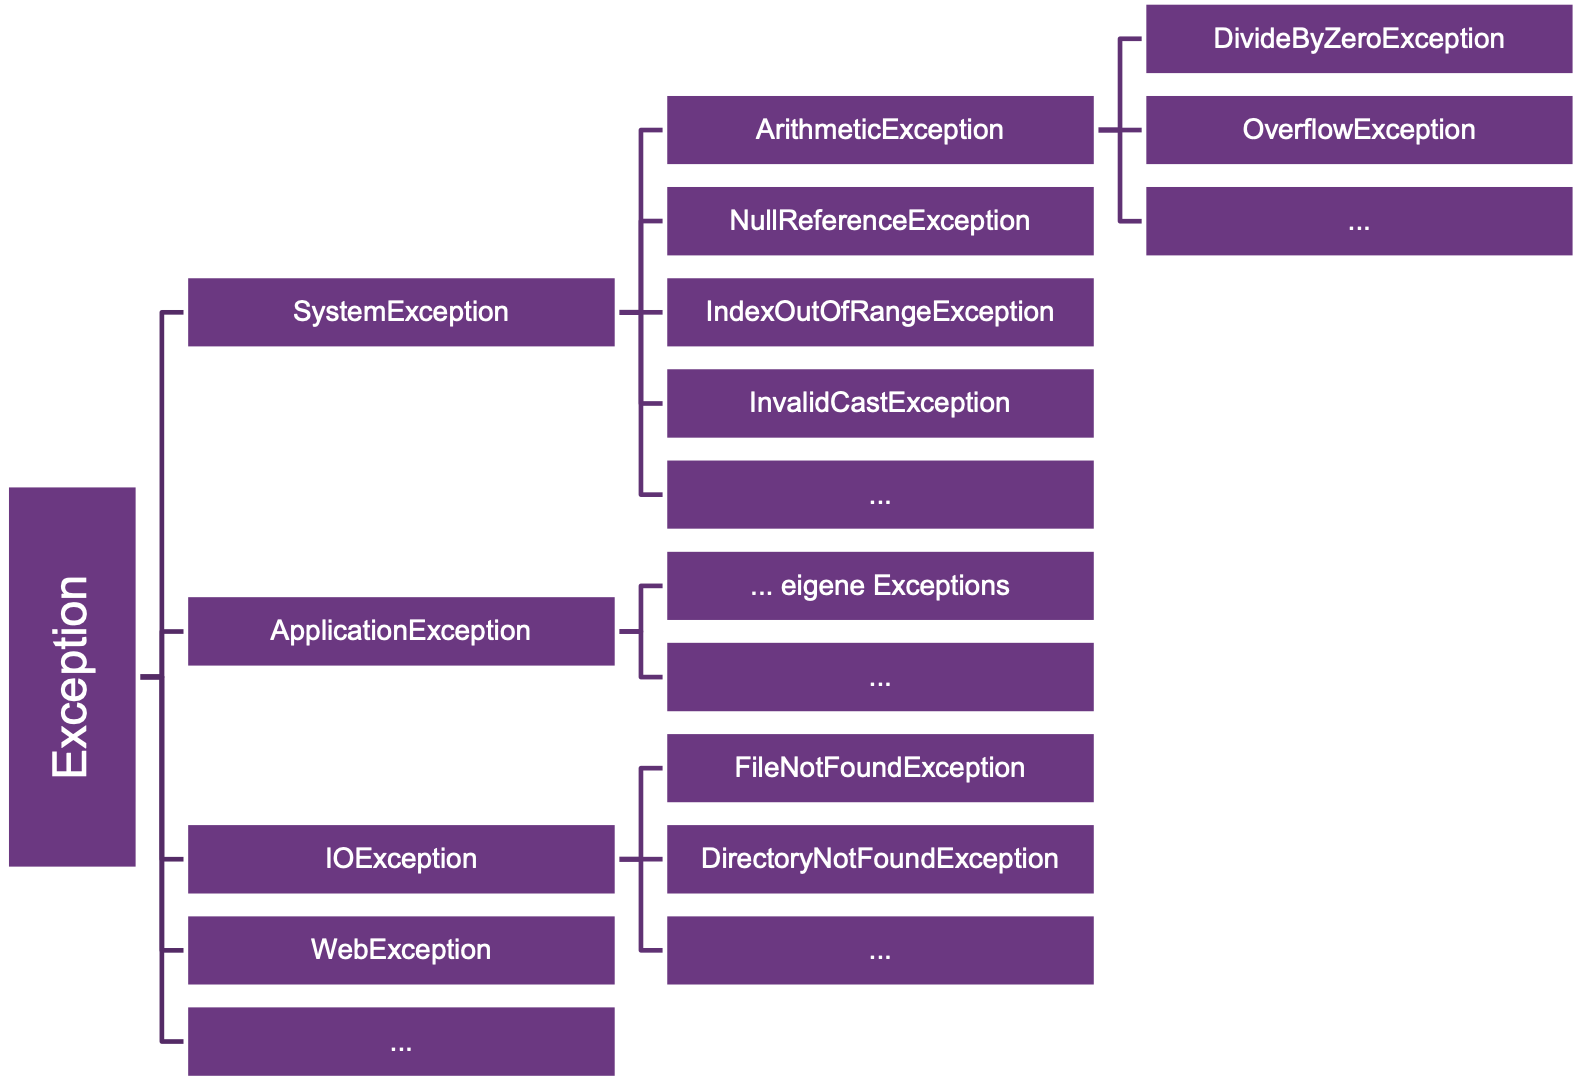
\includegraphics[scale=.25]{graphic/exceptions/Exception-Typen.png}
\end{center}
\vspace{-8pt}

\subsection{Suche nach catch-Klausel}
\begin{itemize}
    \item Call Stack wird rückwärts nach passender «catch» Klausel durchsucht
    \item Programmabbruch mit Fehlermeldung und Stack-Trace falls nicht gefunden
\end{itemize}
\vspace{-8pt}
\begin{center}
    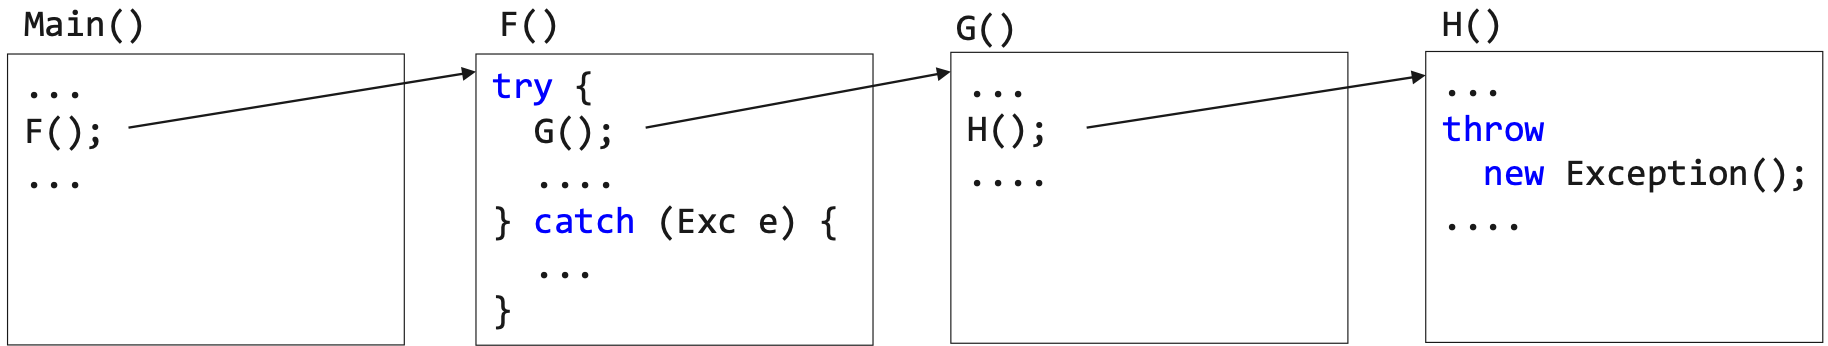
\includegraphics[scale=.25]{graphic/exceptions/Suche.png}
\end{center}
\vspace{-8pt}

\subsubsection{mit Delegates}
\begin{itemize}
    \item Delegates werden wie normale Methoden behandelt
\end{itemize}
\vspace{-8pt}
\begin{center}
    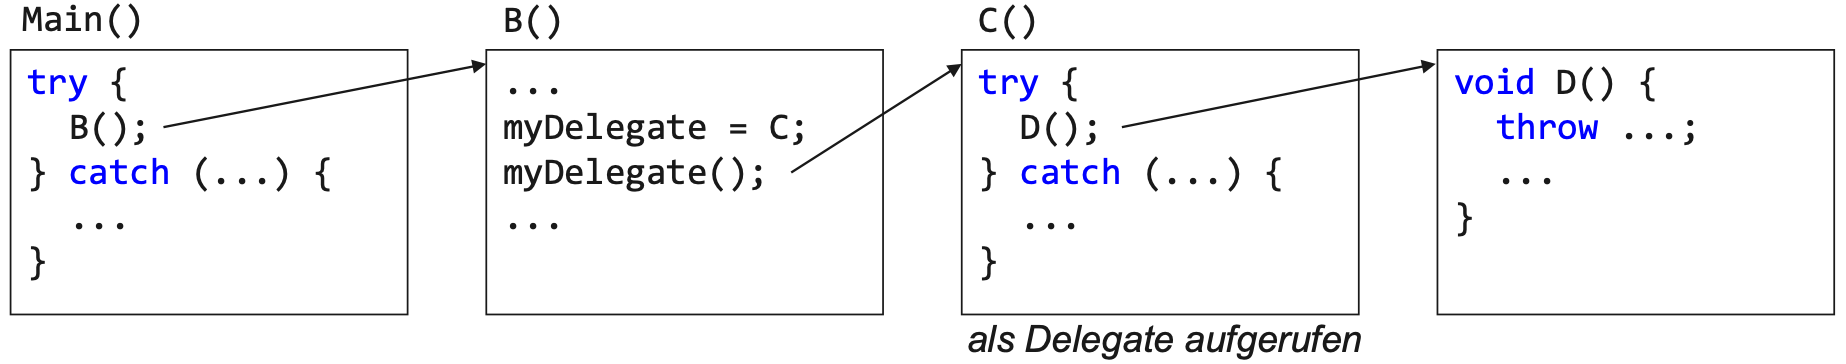
\includegraphics[scale=.25]{graphic/exceptions/suche delegate.png}
\end{center}
\vspace{-8pt}

\subsubsection{mit Multicast-Delegates}
\begin{itemize}
    \item Szenario 1
    \begin{itemize}
        \item Exc1 in G() wird ausgelöst
        \item «catch» für Exc1 in F1() behandelt Ausnahme
        \item F2() wird aufgerufen
    \end{itemize}
    \item Szenario 2
    \begin{itemize}
        \item Exc2 in G() wird ausgelöst
        \item Keine «catch» Klausel für Exc2 gefunden
        \item F2() wird nicht aufgerufen
        \item «catch» für Exc2 in Main() behandelt Ausnahme
    \end{itemize}
\end{itemize}
\vspace{-8pt}
\begin{center}
    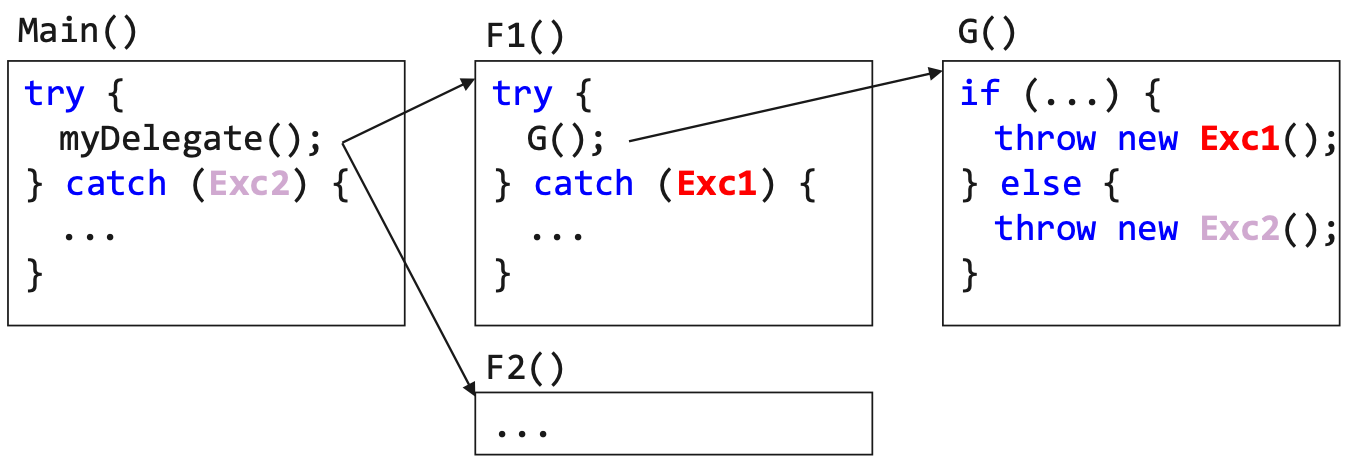
\includegraphics[scale=.27]{graphic/exceptions/suche delegate multicast.png}
\end{center}
\vspace{-8pt}

\subsection{Exception Filters}
Catch-Block wird nur unter definierter Bediungung ausgeführt

\begin{itemize}
    \item «when» Klausel (Zugriff auf Exception möglich)
    \item Erwartet «bool» Expression
\end{itemize}
\begin{lstlisting}
try {
    /* ... */
}
catch (Exception e) when (DateTime.Now.Hour < 18) {
    /* ... */
}
catch (Exception e) when (DateTime.Now.Hour >= 18) {
    /* ... */}
\end{lstlisting}

\subsection{Unchecked Exceptions}
Aufrufer von myMethod() können Exception
behandeln, müssen aber nicht.
\begin{itemize}
    \item Kürzer und bequemer 
    \item Weniger sicher und robust 
\end{itemize}
\begin{lstlisting}
void myMethod() {
    throw new IOException(); }
\end{lstlisting}

\subsection{Argumente prüfen}
Zwei verschiedene Ausprägungen:
\begin{itemize}
    \item ArgumentNullException
    \begin{itemize}
        \item bei null-Werten
    \end{itemize}
    \item ArgumentOutOfRangeException
    \begin{itemize}
        \item bei ungültigen Wertebereichen
    \end{itemize}
\end{itemize}

\hrule

Verwendung des «nameof» Operators:
\begin{itemize}
    \item Zur Ermittlung des ungültigen Parameter
    \item Refactoring-stabil
\end{itemize}

\begin{lstlisting}
string Replicate(string s, int nTimes) {
    if (s == null) {
        throw new ArgumentNullException(nameof(s));
    }
    if (s.Length == 0) {
        throw new ArgumentOutOfRangeException(nameof(s));
    }
    if (nTimes <= 1) {
        throw new ArgumentOutOfRangeException(nameof(nTimes));
    }
 return new StringBuilder().Insert(0, s, nTimes) .ToString();}
\end{lstlisting}

\newpage
	%! Author = mariuszindel
%! Date = 02.11.20

\section{LINQ}


\subsection{Überblick}
Sprach-integrierte Abfragesprache:
\begin{itemize}
    \item Reine Compiler-Technologie
    \item Query-Syntax (ähnlich SQL)
    \item Beliebige Datenstrukturen als Basis
    \item Typensicherheit
    \item Erlaubt «Funktionale Programmierung» mittels «Lambda Expressions»
    \item Erlaubt «Deklarativen Programmierstil» mittels «Anonymous Types» und «Object Initializers»
\end{itemize}
\subsubsection{Architektur}
\begin{center}
    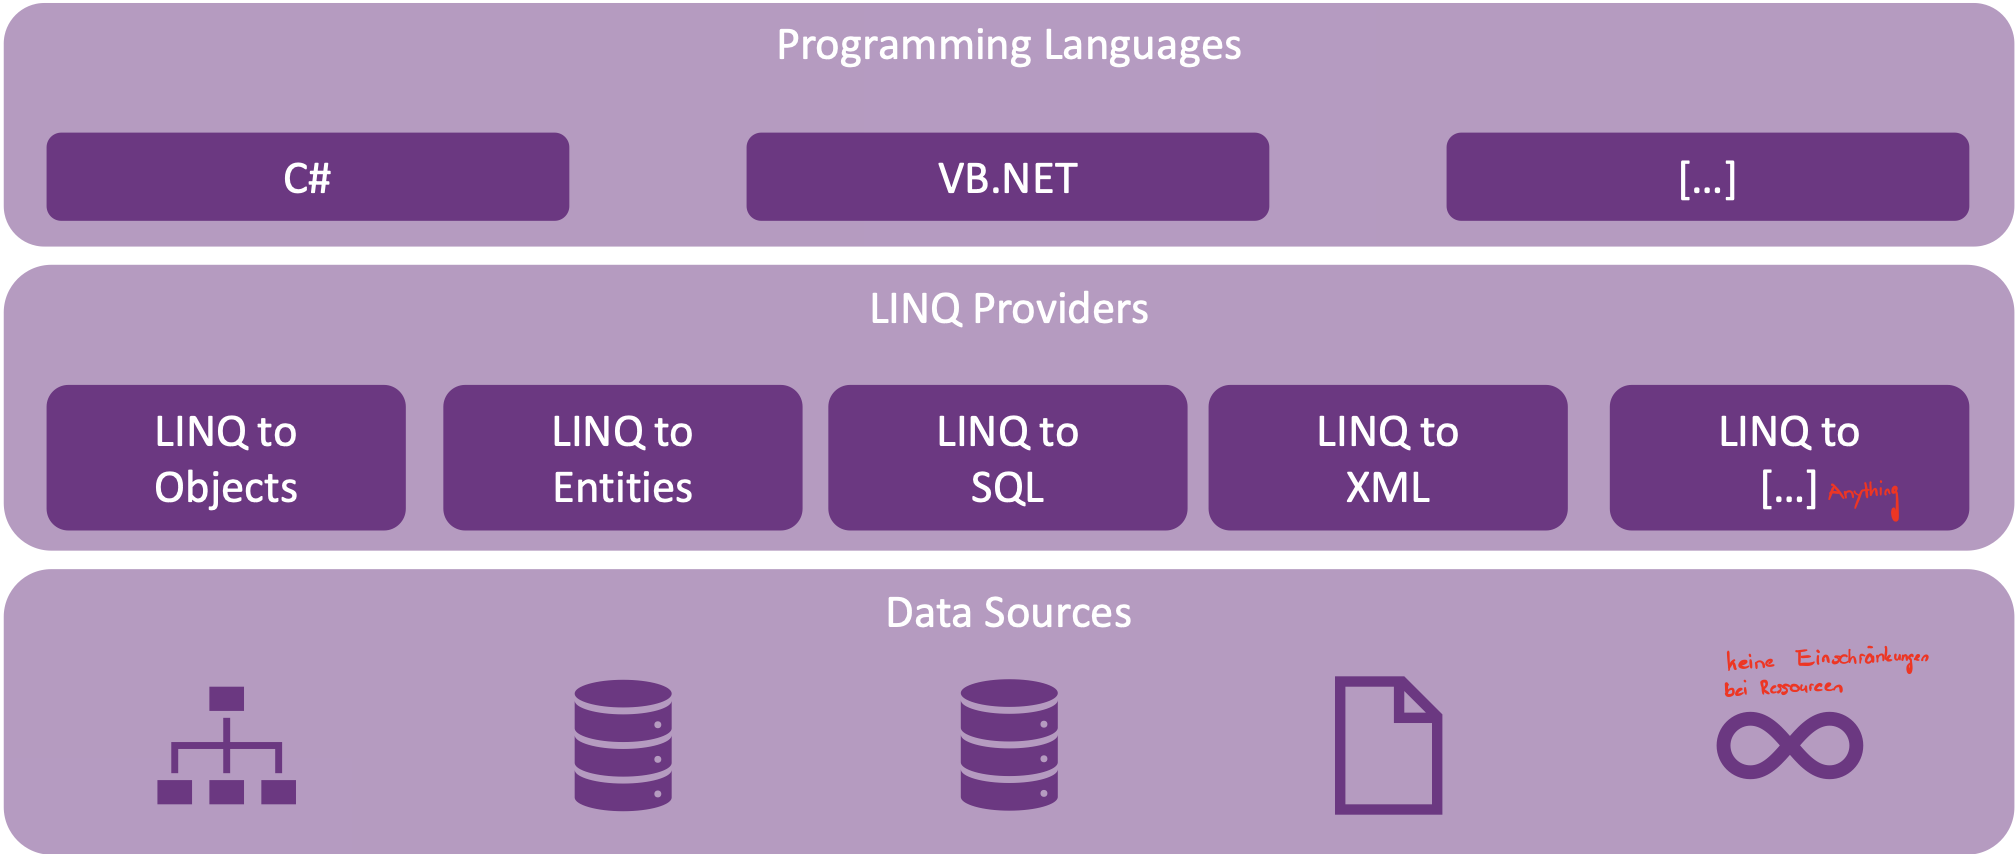
\includegraphics[scale=.2]{graphic/linq/Architektur.png}
\end{center}
\vspace{-8pt}

\subsubsection{Beispiel}
\begin{itemize}
    \item  Abfrage auf Objektstruktur
    \item Query / Lambda Expression 1
    \begin{itemize}
        \item Reine Selektion (ganzes Objekt)
    \end{itemize}
    \item Query / Lambda Expression 2
    \begin{itemize}
        \item Filter nach Namen beginnend mit «B»
        \item Sortierung
        \item Selektion (ganzes Objekt)
    \end{itemize}
    \item Query Expressions werden vom Compiler in Lamda Expressions umgewandelt
\end{itemize}
\vspace{-8pt}
\begin{center}
    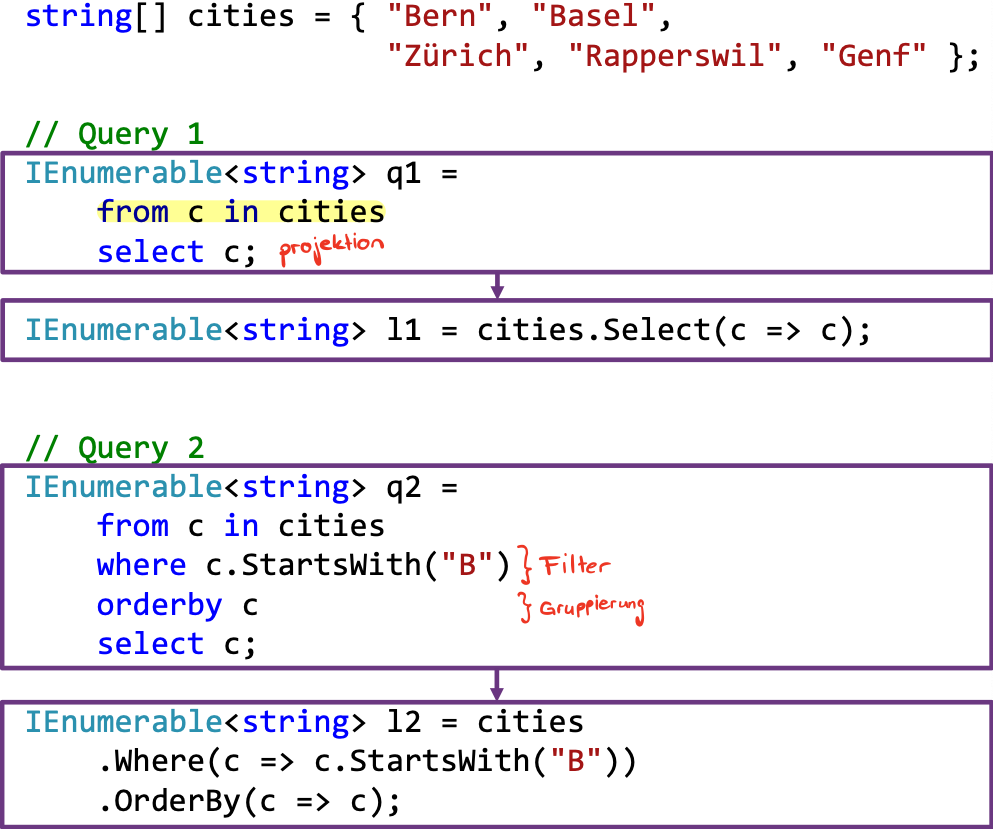
\includegraphics[scale=.35]{graphic/linq/Beispiel LINQ to Objects.png}
\end{center}
\vspace{-8pt}

\subsubsection{Syntax}
\begin{lstlisting}
IEnumerable<string> q2 =
    from c in cities
    where c.StartsWith("B")
    orderby c
    select c;
\end{lstlisting}


\subsection{Lambda Expressions}
\subsubsection{Überblick}
\begin{itemize}
    \item Eine Lambda Expression ist eine Anonyme Methode
    \begin{itemize}
        \item Keine Implementation einer benannten Methode nötig
        \item Kein «delegate» Schlüsselwort mehr nötig
        \item Angabe von Parametertypen optional
    \end{itemize}
    \item Basis für das Erzeugen von
    \begin{itemize}
        \item Delegates
        \item Expression Trees
    \end{itemize}
    \item Zwei Ausprägungen
    \begin{itemize}
        \item Expression Lambdas\\
        («parameters») => expression
        \item Statement Lambdas\\
        («parameters») => { statements; }
    \end{itemize}
\end{itemize}

\begin{lstlisting}
// Expression Lambda
Func<int, bool> fe = i => i % 2 == 0;

// Statement Lambda
Func<int, bool> fs = i => {
    int rest = i%2;
    bool isRestZero = rest == 0;
    return isRestZero;
};
\end{lstlisting}

\subsubsection{Parameter}
\begin{itemize}
    \item Lambdas können 0 – n Parameter haben
    \item Typ-Definition kann oftmals weggelassen werden
    \item Regeln:
    \begin{itemize}
        \item Klammern um Parameter-Definition
        \item «ref» und «out» Parameter sind erlaubt
        \item Jeder Parameter muss implizit in den jeweiligen Delegate-Parameter konvertierbar sein
    \end{itemize}
\end{itemize}
\begin{lstlisting}
Func<bool> p01;
Func<int, bool> p02;
Func<int, int, bool> p03;
Func<int, int, int, bool> p04;

p01 = () => true;          // 0 Parameters
p02 = a => true;           // 1 Parameter
p02 = (a) => true;         // 1 Parameter
p03 = (a, b) => true;      // 2 Parameters
p04 = (a, b, c) => true;   // 3 Parameters // ...

p01 = () => true;                    // 0 Parameters
p02 = int a => true;                 // Compilerfehler
p02 = (int a) => true;               // 1 Parameter
p03 = (int a, int b) => true;        // 2 Parameters
p04 = (int a, int b, int c) => true; // 3 Parameters
\end{lstlisting}

\subsubsection{Type Inference}
\begin{itemize}
    \item Parametertypen sind meist redundant definiert
    \item Somit ist Angabe in Parameterliste obsolet
\end{itemize}
\vspace{-8pt}
\begin{center}
    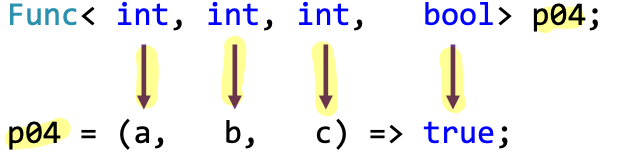
\includegraphics[scale=.33]{graphic/linq/Type Inference.png}
\end{center}
\vspace{-8pt}

\subsubsection{Expression Lambdas}
Syntax:
\begin{lstlisting}
(parameters) => expression

Func<int, int> e1;
e1 = a => a * a;
\end{lstlisting}


\subsubsection{Statement Lambdas}
Syntax:
\begin{lstlisting}
(parameters) => { statements; }

Func<int, int> e1;
e1 = a => { return a * a; };
\end{lstlisting}

\subsubsection{Variable Scope}
Regeln:
\begin{itemize}
    \item Lambda Expression kann auf äussere Variablen zugreifen
    \item Variablen in Lamda Expressions sind für äussere Methoden nicht sichtbar
    \item Zugriff auf «out» und «ref» Parameter nicht erlaubt
\end{itemize}
\begin{lstlisting}
public void TestOuterVariables() {
    int x = 0;
    Action a = () => x = 1;

    Console.WriteLine(x); // Output: 0
    a();
    Console.WriteLine(x); // Output: 1
\end{lstlisting}


\subsection{LINQ Extension Methods}

\subsubsection{Überblick}
\begin{itemize}
    \item LINQ definiert in der Klasse Enumerable eine Vielzahl von Query Operatoren
    \item  Die Methoden in dieser Klasse stellen eine Implementierung von Operatoren zum Abfragen von Datenquellen bereit, die IEnumerable<T> implementieren.
\end{itemize}
\begin{lstlisting}
using System.Linq;

int[] numbers = { 1, 4, 2, 9, 13, 8, 9, 0, -6, 12 };

IEnumerable<int> res = numbers
    .Where(i => i >= 5)
    .OrderBy(i => i);

IEnumerable<int> sqr = numbers
    .Skip(2)
    .Take(4)
    .Select(k=> k * k);
\end{lstlisting}

\subsubsection{Deferred Evaluation}
\begin{itemize}
    \item Query Operatoren sind ebenfalls mit «yield return» implementiert
    \item Queries können beliebig oft ausgeführt werden
\end{itemize}

\subsubsection{Immediate Evaluation}
Einige Operatoren führen Queries direkt aus $\rightarrow$ Wenn Rückgabewert nicht «IEnumerable» ist:
\begin{itemize}
    \item ToList / ToArray
    \item Count / First
    \item Sum / Average
    \item etc.

\end{itemize}
\begin{lstlisting}
public void TestDeferredEvaluation() {

string[] cities = { "Bern", "Basel", "Zuerich", "Rapperswil", "Genf" };

// Ausfuehrung
List<string> citiesB = cities
    .Where(c => c.StartsWith("B"))
    .ToList();

// Ausfuehrung
int citiesEndL = cities
    .Where(c => c.EndsWith("l"))
    .Count();}
\end{lstlisting}


\subsection{Expression-bodied Members}
\begin{itemize}
    \item Allgemein
    \begin{itemize}
        \item Lambda-Expression anstelle von Block { }
        \item Darf aus maximal einem Statement bestehen
    \end{itemize}
    \item Funktioniert für
    \begin{itemize}
        \item Methoden / Operatoren
        \item Konstruktoren / Destruktoren
        \item Properties / Indexers
    \end{itemize}
    \item Spezialfall «Properties»
    \begin{itemize}
        \item Read-Only Properties brauchen keinen Statement-Block { }
        \item Get/Set- und reine Set-Properties schon
    \end{itemize}
\end{itemize}


\subsection{Object / Collection Initializers}

\subsubsection{Object Initializers}
\begin{itemize}
    \item Erlaubt das Instanzieren und Initialisieren einer Klasse in einem Statement
    \item  Reine Compiler-Technologie
\end{itemize}
\begin{lstlisting}
class Student {
    public string Name;
    public int Id;
    public string Subject { get; set; }
    public Student() { }
    public Student(string name) { Name = name; }
}

class Examples {
    public void Test() {
        Student s1 = new Student("John") {
            Id = 2009001, // Set public field
            Subject = "Computing" // Set property
        };
        int[] ids = { 2009001, 2009002, 2009003 };
        IEnumerable<Student> students = ids
            .Select(n => new Student { Id = n });}
}}
\end{lstlisting}

\subsubsection{Collection Initializers (Collections)}
Erlaubt das Instanzieren und Initialisieren einer Collection in einem Statement:
\begin{lstlisting}
//Syntax:
new collection
{ elem1 , ..., elemN };

//Bsp:
class Examples {
public void Test() {
    List<int> l1 = new List<int>
        { 1, 2, 3, 4 }
\end{lstlisting}

\subsubsection{Collection Initializers (Dictionaries)}
Erlaubt das Instanzieren und Initialisieren eines Dictionaries in einem Statement:
\begin{lstlisting}
//Syntax:
new dictionary
{ { key1, v1 }, ...,
    { keyN, vN } };

//Bsp:
class Examples {
    public void Test() {
        Dictionary<int, string> d1 = new Dictionary<int, string>
            {
                { 1, "a" },
                { 2, "b" },
                { 3, "c" }
            };
    }}
\end{lstlisting}

\subsubsection{Kombination}
\begin{itemize}
    \item Object und Collection Initializers lassen sich beliebig kombinieren
    \item Wird oft auch für GUI-Aufbau oder Test-Datenstrukturen verwendet
\end{itemize}
\begin{lstlisting}
object s = new Dictionary<int, Student> {

{ 2009001, new Student("John") {
    Id = 2009001, Subject = "Computing" } },

{ 2009002, new Student {
    Name = "Ann", Id = 2009002, Subject = "Mathematics" } }
};
\end{lstlisting}


\subsection{Anonymous Types}

\subsubsection{Schlüsselwort «var» / Type Inference}
\begin{itemize}
    \item Typ einer Variable muss nicht mehr angegeben
    \item «var» wird anstelle des Typen verwendet
    \item Deklaration und Initialisierung müssen im gleichen Statement sein
    \item Schlüsselwort «var»
    \begin{itemize}
        \item wird vom Compiler durch korrekten Typen ersetzt
        \item kann nur für lokale Variablen verwendet werden
        \item kann nicht als Parameter, Klassen-Variable, Property-Typ, etc.
    \end{itemize}
    \item Im IL-Code steht der effektive Typ
\end{itemize}

\subsubsection{Überblick}
\begin{itemize}
    \item Erzeugung eines Strukturierten Wertes
    \item Meist in LINQ Queries verwendet (Projektion)
\end{itemize}

\subsubsection{Syntax}
\begin{lstlisting}
var a = new { Id = 1, Name = "John" };
var b = new { a.Id, a.Name };
\end{lstlisting}




\section{LINQ Query Expressions}

\subsection{Einführung}
\subsubsection{Überblick}
\begin{itemize}
    \item SQL-ähnliche Syntax
    \item Bestandteile einer Query Operation
    \begin{itemize}
        \item Datenquelle wählen 
        \item Query definieren 
        \item Query gegen Datenquelle ausführen
    \end{itemize}
\end{itemize}
\begin{lstlisting}
// 1. Datenquelle waehlen
int[] numbers = { 0, 1, 2, 3, 4, 5, 6 };

// 2. Query erstellen
var numQuery =
    from num in numbers
    where (num % 2) == 0
    select num;

// 3. Query ausfuehren
foreach (int num in numQuery) {
    Console.Write("{0,1} ", num);
}
\end{lstlisting}

\subsubsection{Query Syntax}
7 Query-Schlüsselwörter:
\begin{enumerate}
    \item from: Definiert eine Range-Variable und eine Datenquelle
    \item where: Filter
    \item orderby: Sortierung
    \item select: Projektion auf einen Elementtypen
    \item group: Gruppierung in eine Sequenz von Gruppen-Elementen 
    \item join: Verknüpfung zweier Datenquellen
    \item let: Definition von Hilfsvariablen
\end{enumerate}
\begin{lstlisting}
var q1 = from s in Students
    where s.Subject == "Computing"
    orderby s.Name
    select new { s.Id, s.Name };
\end{lstlisting}
\begin{itemize}
    \item beginnt immer mit «from»
    \item endet immer mit «select» oder «group»
\end{itemize}

\subsection{Abfragen}
\subsubsection{Query Operatoren / Extension Methoden}
\begin{center}
    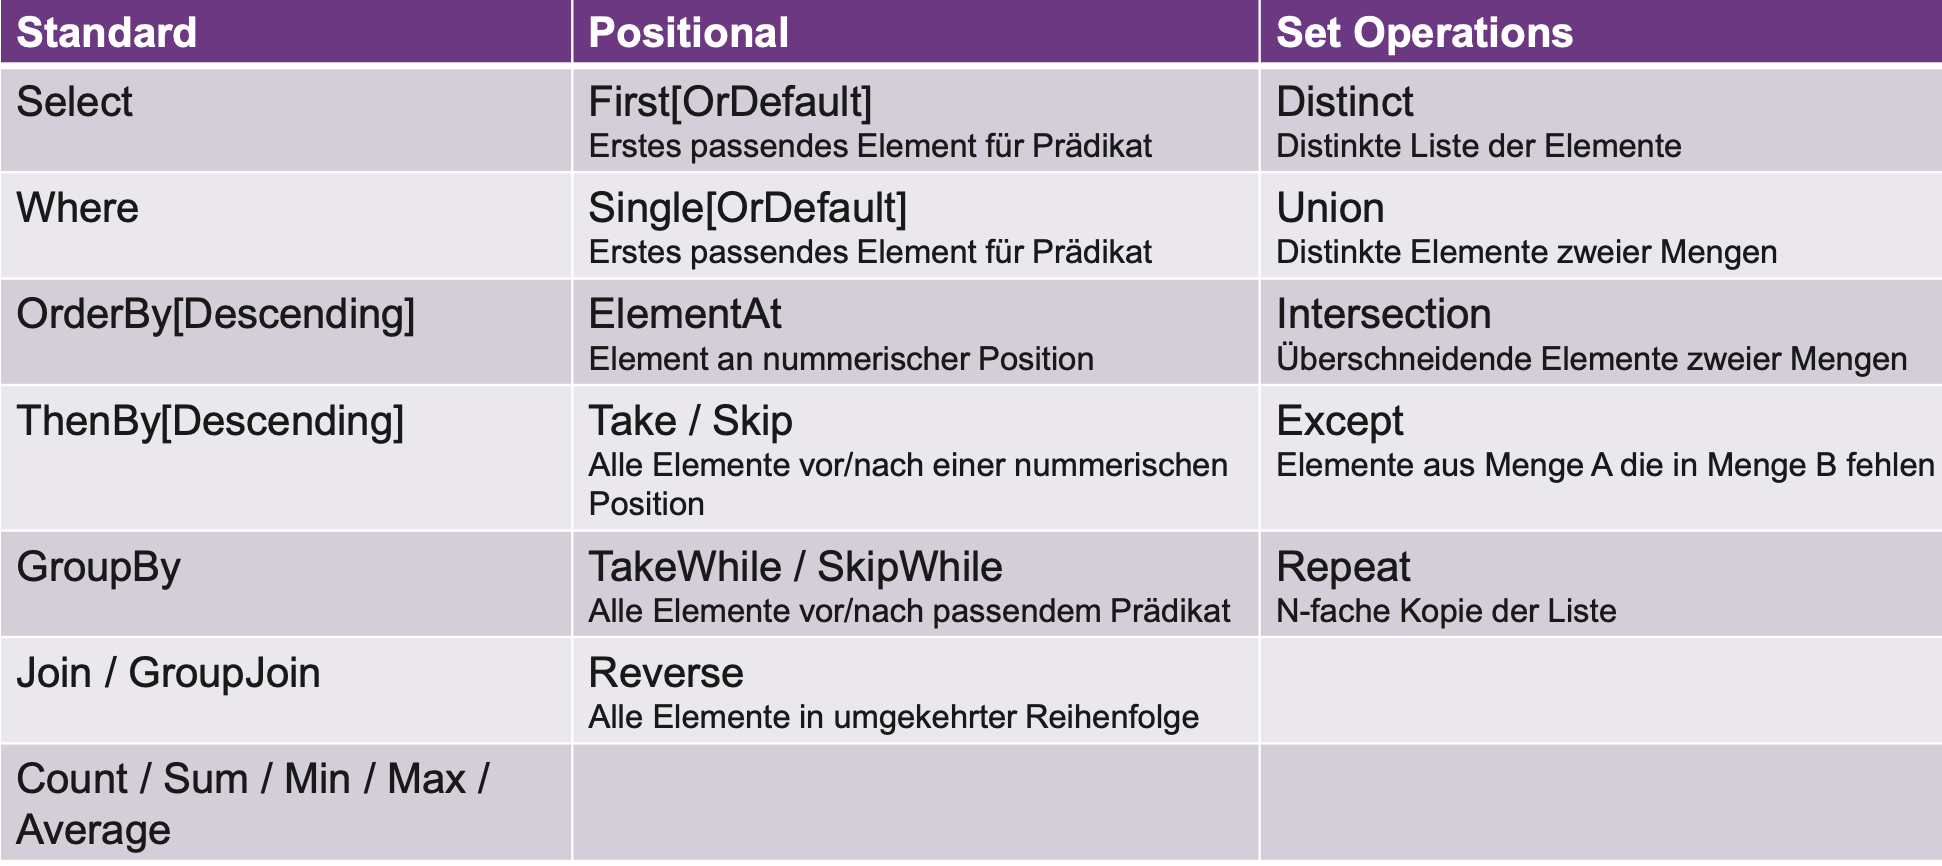
\includegraphics[width=\linewidth]{graphic/linq/Query Operatoren.png}
\end{center}
\vspace{-8pt}

\subsubsection{Range Variablen}
\begin{itemize}
    \item Enstehen durch folgende Klauseln:
    \begin{itemize}
        \item from
        \item join
        \item into
    \end{itemize}
    \item Sind «readonly»
\end{itemize}
\vspace{-8pt}
\subsubsection{Query Operatoren / Extension Methoden}
\begin{center}
    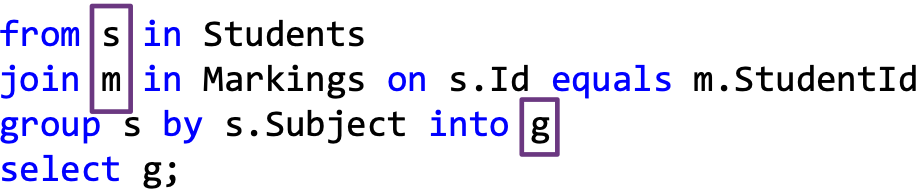
\includegraphics[scale=.3]{graphic/linq/Range Variablen.png}
\end{center}
\vspace{-8pt}

\subsubsection{Gruppierung}
\begin{itemize}
    \item Transformation in «Key/Value Pairs»
    \item Zusammenfassung in ein IEnumerable der Gruppen nach «Key»
\end{itemize}
\vspace{-8pt}
\begin{center}
    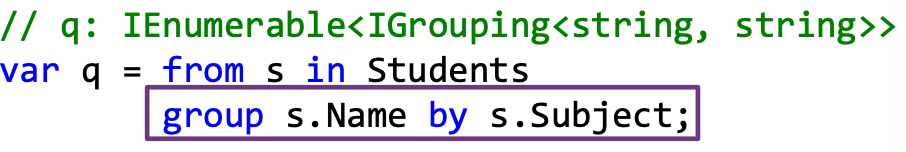
\includegraphics[scale=.3]{graphic/linq/Gruppierung.png}
\end{center}
\vspace{-8pt}

\subsubsection{Gruppierung / Direkte Weiterverwendung}
«into» speichert Resultat in Variable «g»
\begin{itemize}
    \item «s» ist danach nicht mehr sichbar
    \item «g» kann als Gruppe weiterverwendet werden
\end{itemize}
\vspace{-8pt}
\begin{center}
    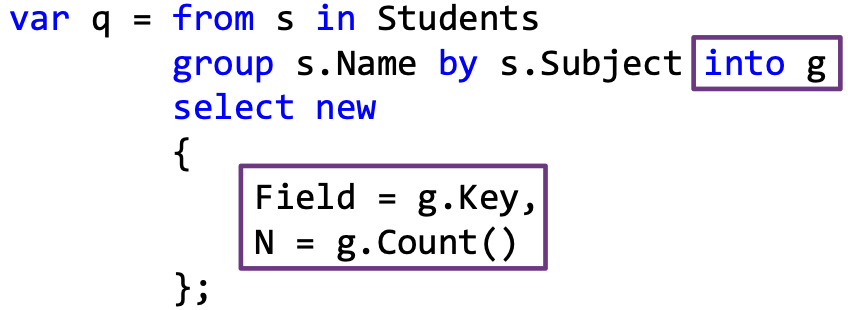
\includegraphics[scale=.3]{graphic/linq/Gruppierung Direkte Weiterverwendung.png}
\end{center}
\vspace{-8pt}

\subsubsection{Inner Joins / Explizit}
\begin{itemize}
    \item Verknüpft zwei Mengen über einen Schlüssel
    \item Zwingend mit «equals» verknüpfen (nicht mit ==)
\end{itemize}
\vspace{-8pt}
\begin{center}
    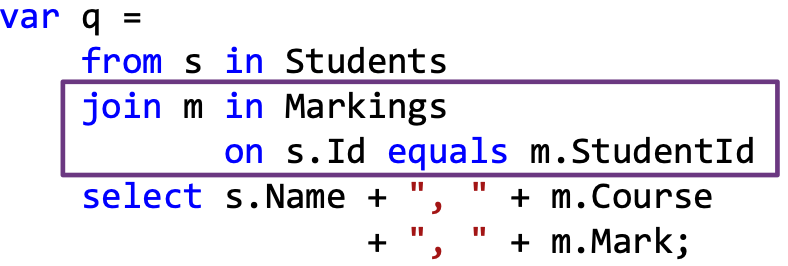
\includegraphics[scale=.3]{graphic/linq/inner join.png}
\end{center}
\vspace{-8pt}

\subsubsection{Inner Joins / Implizit}
\begin{itemize}
    \item Verknüpft zwei Mengen über einen Schlüssel
    \item Unterschied: Weniger effizient
    \begin{itemize}
        \item Bildet Kreuzprodukt
        \item Reduziert Kreuzprodukt bei zutreffender «where» Klausel
    \end{itemize}
\end{itemize}
\vspace{-8pt}
\begin{center}
    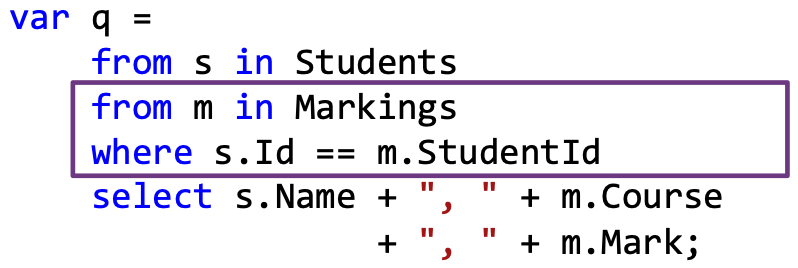
\includegraphics[scale=.3]{graphic/linq/inner join implizit.png}
\end{center}
\vspace{-8pt}

\subsubsection{Group Joins}
\begin{itemize}
    \item Pro «Student» wird eine Liste für alle «Markings» erstellt
    \item «s» bleibt sichtbar
\end{itemize}
\vspace{-8pt}
\begin{center}
    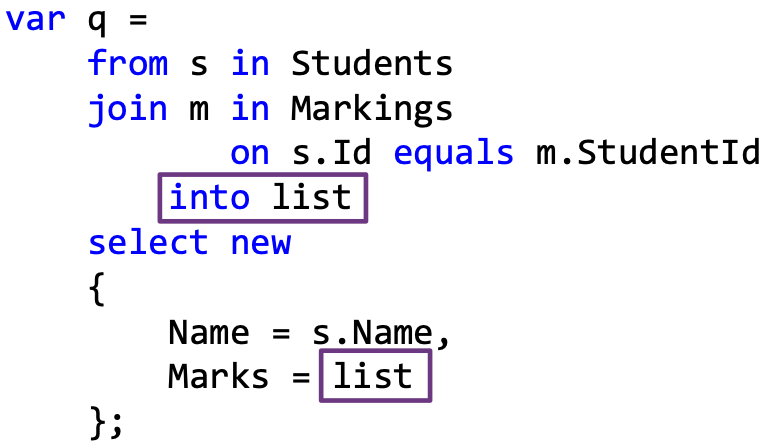
\includegraphics[scale=.3]{graphic/linq/Group Joins.png}
\end{center}
\vspace{-8pt}

\subsubsection{Left Outer Joins}
\begin{itemize}
    \item Verknüpft zwei Mengen über einen Schlüssel
    \item Wenn kein rechtes Element gefunden wird bleibt linkes Element trotzdem bestehen
\end{itemize}
\vspace{-8pt}
\begin{center}
    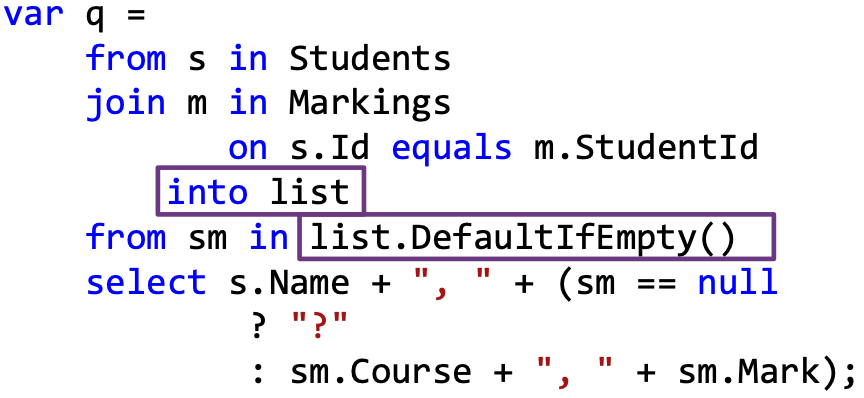
\includegraphics[scale=.3]{graphic/linq/Left Outer Joins.png}
\end{center}
\vspace{-8pt}

\subsubsection{let Klausel}
\begin{itemize}
    \item Erlaubt das Definieren von Hilfsvariablen
\end{itemize}
\vspace{-8pt}
\begin{center}
    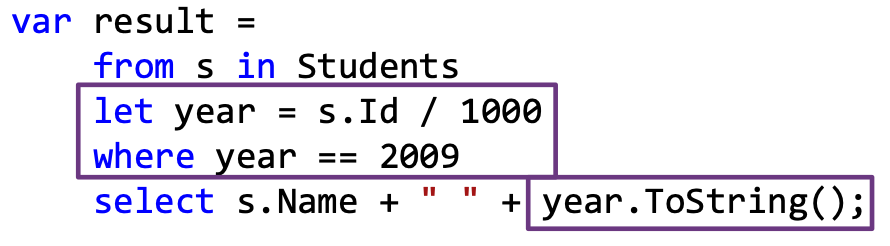
\includegraphics[scale=.3]{graphic/linq/let Klausel.png}
\end{center}
\vspace{-8pt}

\subsubsection{Select Many}
\begin{itemize}
    \item Erleichtert das zusammenfassen verschachtelter Listen
    \item Für jedes Listenelement auf oberster Stufe den «selector» aus
    \item Dieser liefert selbst eine Liste (Teilliste)
    \item Teillisten werden untereinander gehängt
\end{itemize}
\vspace{-8pt}
\begin{center}
    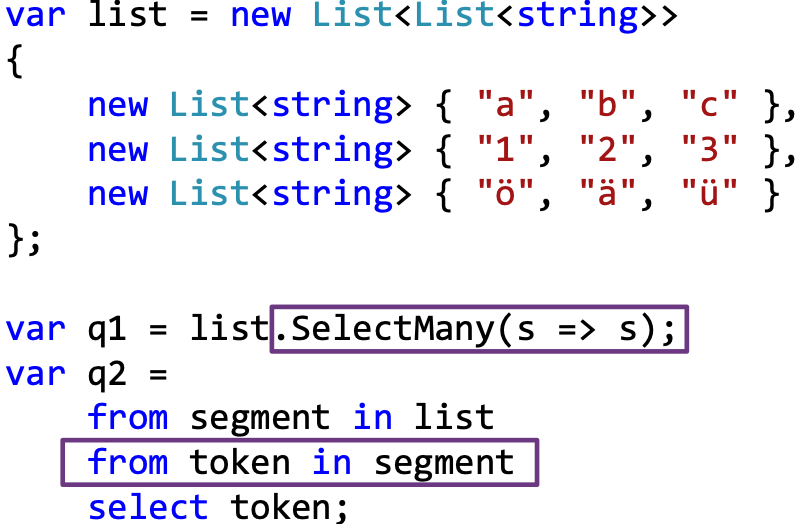
\includegraphics[scale=.3]{graphic/linq/Select Many.png}
\end{center}
\vspace{-8pt}


\newpage
	%! Author = mariuszindel
%! Date = 02.11.20

\section{Entity Framework Core}


\subsection{Überblick}
\begin{itemize}
    \item Entity Framework Core / EF Core ist ein O/R Mapping Framework
    \begin{itemize}
        \item Verbindet Objekt-Orientiertes (Domain Model)
        \item mit Relationalem (Relational Model)
    \end{itemize}
    \item Diverse Basis-Funktionalitäten
    \begin{itemize}
        \item Mapping von Entitäten
        \item CRUD Operationen (Create, Read, Update, Delete
        \item Key-Generierung
        \item Caching
        \item Change Tracking
        \item Optimistic Concurrency
        \item Transactions
        \item Command Line Interface
    \end{itemize}
\end{itemize}


\subsection{OR-Mapping}

\subsubsection{Providers}
\begin{center}
    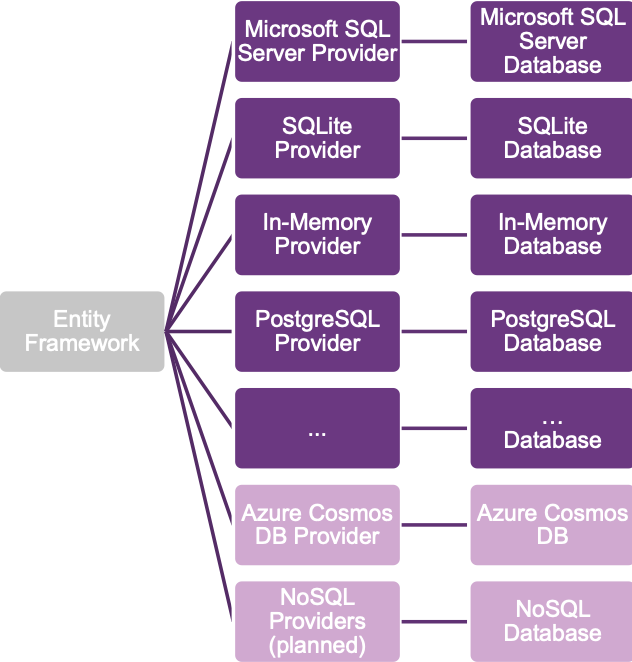
\includegraphics[scale=.4]{graphic/efc/providers.png}
\end{center}
\vspace{-8pt}

\subsubsection{Überblick}
\begin{itemize}
    \item Entity Type
    \begin{itemize}
        \item Domain Modell / Konzeptionelles Modell / etc.
        \item Normale .NET Klassen
    \end{itemize}
    \item Mapping - Drei verschiedene Ansätze:
    \begin{itemize}
        \item By Convention
        \item By Attributes
        \item By Fluent API
    \end{itemize}
    \item Storage Entity
    \begin{itemize}
        \item Relationales Modell / Graph / Collection / etc.
        \item Abhängig von gewähltem Provider
    \end{itemize}
\end{itemize}
\vspace{-8pt}
\begin{center}
    \includegraphics[scale=.3]{graphic/efc/überblick.png}
\end{center}
\vspace{-8pt}

\subsubsection{Entrity Type}
\begin{itemize}
    \item Ausprägung
    \begin{itemize}
        \item Klasse
    \end{itemize}
    \item Inhalte
    \begin{itemize}
        \item Properties (Name)
        \item Entry Keys (Primary Key)
        \item Alternative Keys
        \item Relationships
        \item Foreign Keys
    \end{itemize}
\end{itemize}

\subsubsection{Storage Entity}
\begin{itemize}
    \item Ausprägung
    \begin{itemize}
        \item Table
        \item View
        \item Stored Procedures
    \end{itemize}
    \item Inhalte
    \begin{itemize}
        \item Columns
        \item Primary Keys
        \item Unique Key Constraints
        \item Foreign Keys
    \end{itemize}
\end{itemize}

\subsubsection{Mapping}
\begin{itemize}
    \item Zuordnung von
    \begin{itemize}
        \item Entity Type zu Storage Entity
        \item Property zu Column
        \item Entity Key zu Primary Key
        \item Foreign Key zu Relationship
    \end{itemize}
    \item Erweiterte Szenarien
    \begin{itemize}
        \item Vererbung / Inheritance
        \item Table Split / Table Merge
        \item Complex Types
    \end{itemize}
    \item Ausprägungen
    \begin{itemize}
        \item By Convention
        \item By Attributes
        \item By Fluent API
    \end{itemize}
\end{itemize}

\subsubsection{Mappingarten (Entity-Level)}
\begin{center}
    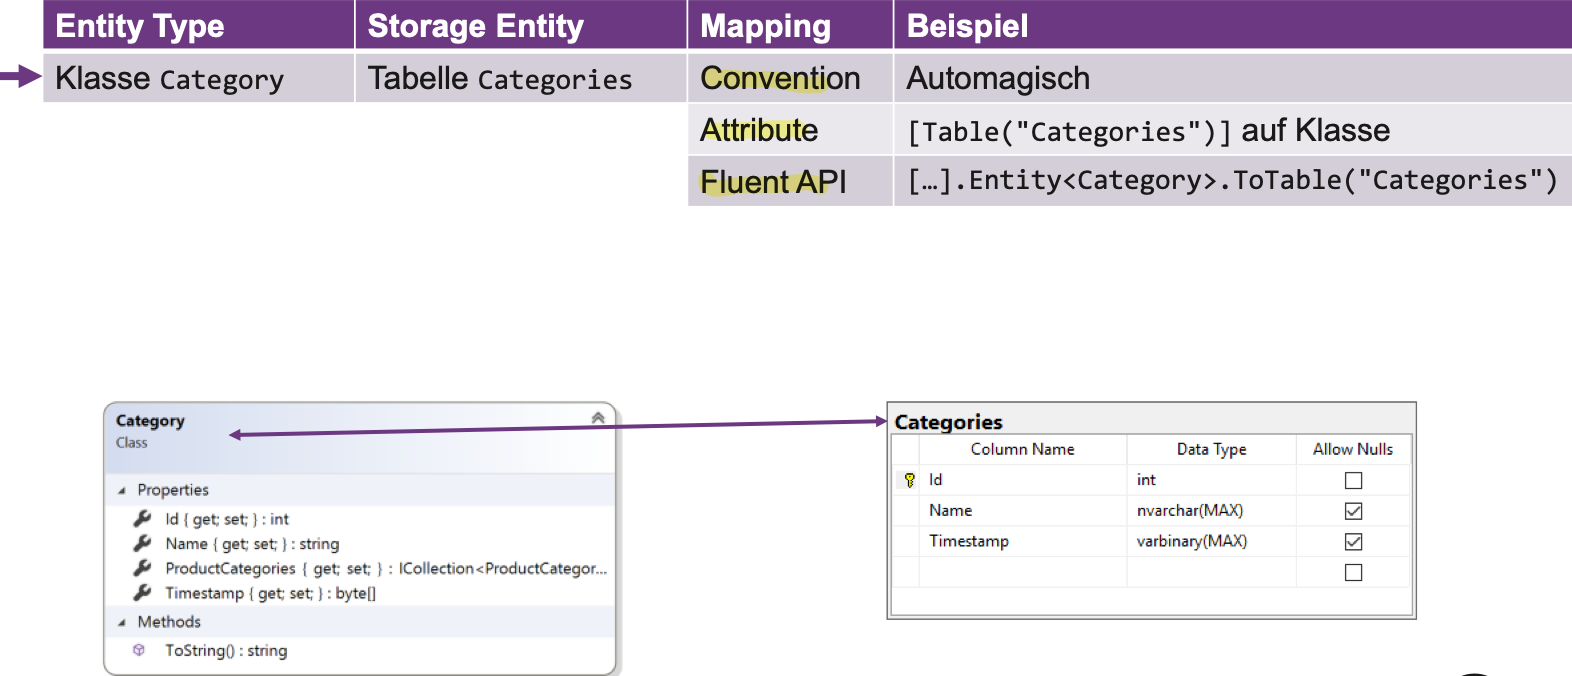
\includegraphics[scale=.32]{graphic/efc/Entity-Level.png}
\end{center}
\vspace{-8pt}

\subsubsection{Mappingarten (Attribut-Level)}
\begin{center}
    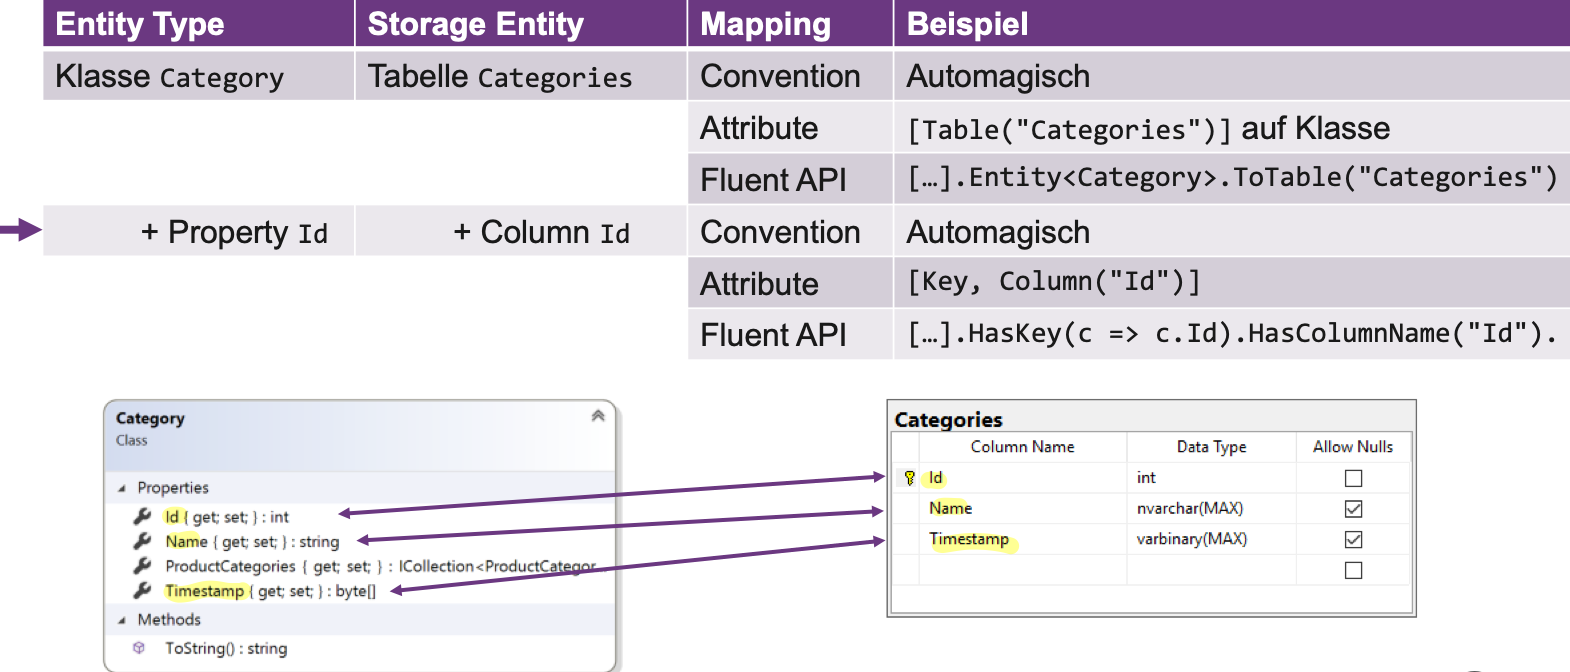
\includegraphics[scale=.32]{graphic/efc/Attribut-Level.png}
\end{center}
\vspace{-8pt}

\subsection{Ansätze}
\begin{center}
    \includegraphics[scale=.3]{graphic/efc/ansätze.png}
\end{center}
\vspace{-8pt}


\subsection{OR-Mapping Modell}
\subsubsection{Überblick}
\begin{itemize}
    \item Mapping by Convention
    \begin{itemize}
        \item Automatisches Mapping ohne explizite Konfiguration
    \end{itemize}
    \item Mapping by Fluent API
    \begin{itemize}
        \item Extension-Method-Syntax
        \item Überschriebene Methode von «OnModelCreating» im DbContext
    \end{itemize}
    \item Mapping by Data Annotations
    \begin{itemize}
        \item Deklaratives Mapping
        \item Attribute direkt auf Model-Klassen
        \item Namespace
    \end{itemize}
\end{itemize}

\subsubsection{Include / Exclude von Entities}
\begin{center}
    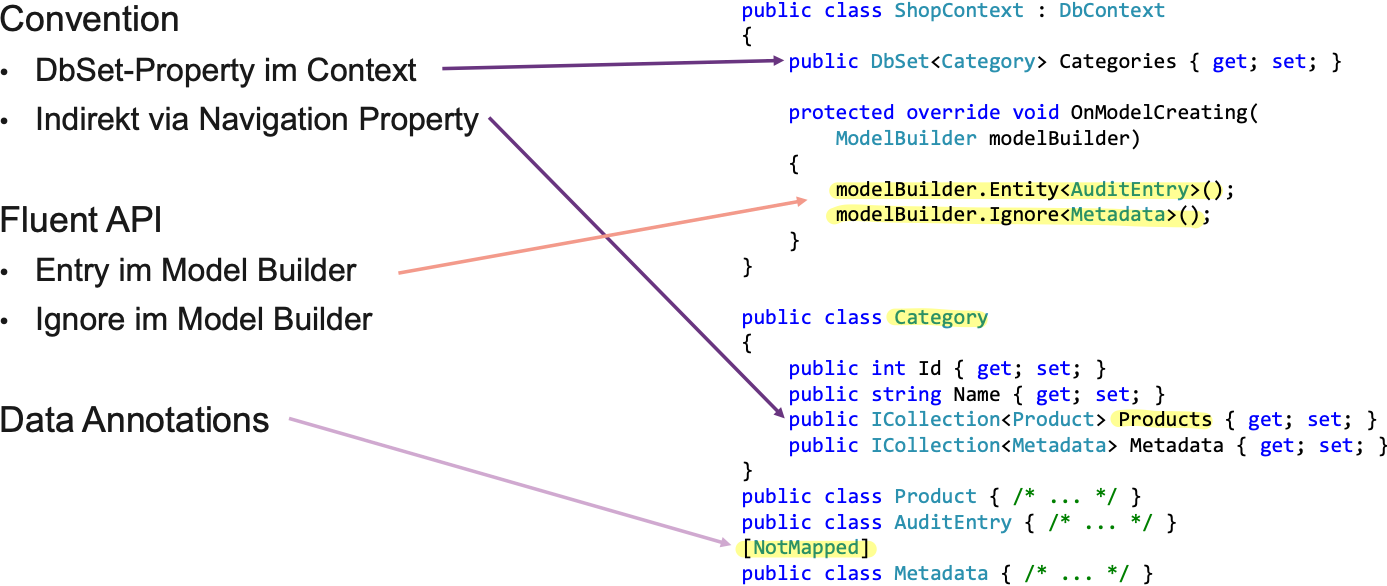
\includegraphics[scale=.35]{graphic/efc/Include Exclude von Entities.png}
\end{center}
\vspace{-8pt}

\subsubsection{Include / Exclude von Properties}
\begin{center}
    \includegraphics[scale=.35]{graphic/efc/Include Exclude von Properties.png}
\end{center}
\vspace{-8pt}

\subsubsection{Keys}
\begin{center}
    \includegraphics[scale=.37]{graphic/efc/Keys.png}
\end{center}
\vspace{-8pt}

\subsubsection{Required / Optional}
\begin{center}
    \includegraphics[scale=.37]{graphic/efc/Required Optional.png}
\end{center}
\vspace{-8pt}

\subsubsection{Maximum Length}
\begin{center}
    \includegraphics[scale=.37]{graphic/efc/Maximum Lengt.png}
\end{center}
\vspace{-8pt}

\subsubsection{Indexes}
\begin{center}
    \includegraphics[scale=.36]{graphic/efc/Indexes.png}
\end{center}
\vspace{-8pt}

\subsubsection{Entity Type Configuration}
\begin{center}
    \includegraphics[scale=.37]{graphic/efc/Entity Type Configuration.png}
\end{center}
\vspace{-8pt}


\subsection{OR-Mapping: Relationale Datenbank (SQL Server)}

\subsubsection{Tabellen}
\begin{center}
    \includegraphics[scale=.37]{graphic/efc/tabellen.png}
\end{center}
\vspace{-8pt}

\subsubsection{Spalten}
\begin{center}
    \includegraphics[scale=.37]{graphic/efc/Spalten.png}
\end{center}
\vspace{-8pt}

\subsubsection{Datentypen / Default Values}
\begin{center}
    \includegraphics[scale=.37]{graphic/efc/Datentypen Default Values.png}
\end{center}
\vspace{-8pt}

\subsubsection{Relationship – one-to-many / Fully Defined}
\begin{center}
    \includegraphics[scale=.37]{graphic/efc/Relationship – one-to-many Fully Defined.png}
\end{center}
\vspace{-8pt}

\subsubsection{Relationship – one-to-many / No Foreign Key Property}
\begin{center}
    \includegraphics[scale=.37]{graphic/efc/Relationship – one-to-many No Foreign Key Property.png}
\end{center}
\vspace{-8pt}

\subsubsection{Relationship – one-to-many / Single Navigation Property}
\begin{center}
    \includegraphics[scale=.37]{graphic/efc/Relationship – one-to-many Single Navigation Property.png}
\end{center}
\vspace{-8pt}

\subsubsection{Relationship – one-to-many / Foreign Key}
\begin{center}
    \includegraphics[scale=.36]{graphic/efc/Relationship – one-to-many Foreign Key.png}
\end{center}
\vspace{-8pt}

\subsubsection{Relationship – one-to-one / many-to-many}
\begin{center}
    \includegraphics[scale=.3]{graphic/efc/Relationship – one-to-one many-to-many.png}
\end{center}
\vspace{-8pt}

\subsubsection{Relationship – Diverses}
\begin{center}
    \includegraphics[scale=.31]{graphic/efc/Relationship – Diverses.png}
\end{center}
\vspace{-8pt}

\subsubsection{Diverses}
\begin{center}
    \includegraphics[scale=.33]{graphic/efc/Diverses.png}
\end{center}
\vspace{-8pt}


\subsection{Database Context}

\subsubsection{Überblick}
\begin{itemize}
    \item Wichtigster Teil des Entity Framework
    \item Kombination zweier Patterns
    \begin{itemize}
        \item Repository + Unit of Work
    \end{itemize}
    \item Funktionen:
    \begin{itemize}
        \item Design-Time
        \begin{itemize}
            \item Model definieren (OR-Mapping)
            \item Konfiguration
            \item Database Migrations
        \end{itemize}
        \item Run-Time
        \begin{itemize}
            \item Connections verwalten (Connection Pool)
            \item CRUD Operationen ausführen
            \item Change Tracking
            \item Caching
            \item Transaction Management
        \end{itemize}
    \end{itemize}
\end{itemize}

\subsubsection{DbContext Lifecycle}
DbContext-Instanzen sollten nicht
\begin{itemize}
    \item zu lange leben
    \begin{itemize}
        \item Limitierte Anzahl Connections im Client Connection Pool
        \item Change-Tracking wird über die Zeit ineffizient
    \end{itemize}
    \item geshared werden
    \begin{itemize}
        \item Ist nicht thread-safe
        \item Exception kann Instanz unbrauchbar machen
    \end{itemize}
\end{itemize}

Empfehlungen:
\begin{itemize}
    \item In einem «using»-Statement verwenden
    \item Web Applikationen: Instanz pro Request
    \item GUI: Instanz pro Formular
    \item Generell: Instanz pro «Unit of Work»
\end{itemize}
\begin{lstlisting}
// So verwenden:
using (ShopContext context = new ShopContext()) { Query... }
\end{lstlisting}


\subsection{Query Execution with JOIN}
\begin{center}
    \includegraphics[scale=.35]{graphic/efc/join.png}
\end{center}
\vspace{-8pt}

\subsection{Database Context: CUD Operatoren}
\subsubsection{Insert}
\begin{lstlisting}
using (ShopContext context = new ShopContext()) {
    Category cat = new Category
        { Name = "Notebooks" };

    // Add to Context (3 alternatives)
    context.Add(cat);
    context.Categories.Add(cat);
    context.Entry(cat).State = EntityState.Added;

    // Save - SQL is executed here
    await context.SaveChangesAsync();

    // Check Primary Key
    int id = cat.Id; // Category.Id is populated
}
\end{lstlisting}

\subsubsection{Update}
\begin{lstlisting}
using (ShopContext context = new ShopContext()) {
    Category cat = await context
        .Categories
        .FirstAsync(); £$\rightarrow$ .Single(p=>p.Name == "Hans");£

    // Change
    cat.Name = "Changed";

    // Save - SQL is executed here
    await context.SaveChangesAsync(); £$\rightarrow$ Oder auch ohne Async£
}
\end{lstlisting}

\subsubsection{Delete}
\begin{lstlisting}
using (ShopContext context = new ShopContext()) {
    Category cat = await context
        .Categories
        .FirstAsync(c => c.Name == "Notebooks");

    // Remove (3 alternatives)
    context.Remove(cat);
    context.Categories.Remove(cat);
    context.Entry(cat).State = EntityState.Deleted;

    // Save - SQL is executed here
    await context.SaveChangesAsync();
}
\end{lstlisting}


\subsection{Database Context: Change Relationship II}
\begin{itemize}
    \item Via Navigation Property
    \item Via Foreign Key
\end{itemize}

\subsection{Database Context: Change Tracking}
\subsubsection{Überblick}
Change Tracker:
\begin{itemize}
    \item Registriert alle Ändungen an «getrackten» Entities
    \item Aktualisiert den Entity State
    \item • Agiert komplett «offline»
\end{itemize}
State Handling:
\begin{itemize}
    \item DbContext hat Methoden für das Hinzufügen und das Setzen des States im Change Tracker
    \begin{itemize}
        \item Add()
        \item Remove()
        \item Update()
        \item Unchanged()
    \end{itemize}
    \item Immer mind. 3 Varianten mit gleichem Effekt
    \begin{itemize}
        \item .Add / .Remove / etc. berücksichtigen ganzen Objekt-Graphen 
        \item .Entry(…).State nur die jeweilige Entity
    \end{itemize}
\end{itemize}
\vspace{-8pt}
\begin{center}
    \includegraphics[scale=.3]{graphic/efc/change tracker.png}
\end{center}
\vspace{-8pt}

\subsubsection{State Entries}
\begin{itemize}
    \item Via DbContext.Entry<T>(object)...
    \item Beinhaltet Informationen über
    \begin{itemize}
        \item Status des Objekts
        \item Für alle Properties
        \begin{itemize}
            \item
        \end{itemize}
        \item Entity-specific loading functions
        \item Reload object values from database
        \item Load referenced entities (see explicit lazy loading)
    \end{itemize}
\end{itemize}
\vspace{-8pt}
\begin{center}
    \includegraphics[scale=.44]{graphic/efc/state entries.png}
\end{center}
\vspace{-8pt}

%\columnbreak

\subsection{Database Context: Ladestrategien}

\subsubsection{Überblick}
Was wird beim Laden eines «Order» Objekts geladen?
\begin{lstlisting}
Order order = await context
    .Orders
    .FirstAsync();

var customer = order
    .Customer; // customer is "null"

var items = order
    .Items; // items is "null"
\end{lstlisting}

\subsubsection{Eager Loading (Default)}
\begin{itemize}
    \item Assoziationen werden per se nicht geladen
    \item Include()-Statement für einzelne Assoziationen
    \item Passiert in der gleichen Abfrage per JOIN
\end{itemize}
\vspace{-8pt}
\begin{center}
    \includegraphics[scale=.4]{graphic/efc/eager loading.png}
\end{center}
\vspace{-8pt}

\subsubsection{Explicit Loading}
\begin{itemize}
    \item Assoziationen werden per se nicht geladen
    \item Assoziationen werden explizit nachgeladen
    \item Collections werden komplett geladen
    \item Passiert in separater Abfrage
\end{itemize}
\vspace{-8pt}
\begin{center}
    \includegraphics[scale=.4]{graphic/efc/explicit loading.png}
\end{center}
\vspace{-8pt}

\subsubsection{Lazy Loading}
\begin{itemize}
    \item Assoziationen werden per se nicht geladen
    \item Assoziationen werden bei Zugriff auf Property automatisch nachgeladen
    \item Collections werden komplett geladen / Filtern aber möglich
    \item Passiert in separater Abfrage
\end{itemize}
Problem:
\begin{itemize}
    \item Model-Klassen meist mit Auto-Properties
    \item Wie kann bei Zugriff auf ein Property zusätzliche (Lade-)Logik ausgeführt werden
\end{itemize}
2 Lösungsvarianten:

\subsubsection{Lazy Loading – Manuell}
Auf Auto-Properties verzichten und Logik manuell implementieren
\vspace{-8pt}
\begin{center}
    \includegraphics[scale=.21]{graphic/efc/Lazy Loading – Manuell.png}
\end{center}
\vspace{-8pt}

\subsubsection{Lazy Loading – Proxy}
\begin{itemize}
    \item Dynamic Binding
    \item Navigation Properties mit «virtual» Keyword
    \item EF Core generiert abgeleitete Proxy-Klassen $\rightarrow$ Zur Laufzeit generiert mit «Castle»
    \item Diese enthalten ca. die Logik von Variante 1
\end{itemize}
\vspace{-8pt}
\begin{center}
    \includegraphics[scale=.21]{graphic/efc/Lazy Loading – Proxy.png}
\end{center}
\vspace{-8pt}

\subsection{Optimistic Concurrency}
\subsubsection{Überblick}
\begin{itemize}
    \item Annahme:
    \begin{itemize}
        \item Zwischen Laden und Speichern eines Records wird nicht verändert $\rightarrow$ Beim Speichern prüfen, ob geändert
    \end{itemize}
    \item Alternative: Pessimistic Concurrency
    \begin{itemize}
        \item Datensatz wird für die Dauer der Verarbeitung gesperrt
        \item Probleme
        \begin{itemize}
            \item Deadlocks
            \item Orphaned Locks
            \item Performance
        \end{itemize}
    \end{itemize}
\end{itemize}

\subsubsection{Erkennung von Konflikten: Timestamp}
\begin{itemize}
    \item Pro Record Timestamp / Row Version
    \item Timestamp ist Teil des Datenobjekts
    \item Datenbank-Timestamp = Objekt-Timestamp $\rightarrow$ Ja $\rightarrow$ speichern + timestamp erhöhen
\end{itemize}
\vspace{-8pt}
\begin{center}
    \includegraphics[scale=.38]{graphic/efc/timestamp.png}
\end{center}
\vspace{-8pt}

\subsubsection{Erkennung von Konflikten: Concurrency Tokens / Daten-Versionen}
\begin{itemize}
    \item Beim Ändern der Daten: Originalwerte wegkopieren
    \item Beim Speichern ebenfalls mitgeben
    \item Datenbankwerte = Originalwerte $\rightarrow$ Ja $\rightarrow$ speichern
\end{itemize}
\vspace{-8pt}
\begin{center}
    \includegraphics[scale=.4]{graphic/efc/Concurrency Tokens.png}
\end{center}
\vspace{-8pt}

\subsubsection{Optimistic Concurrency – Konfliktbehandlung}
DbUpdateConcurrencyException beinhaltet fehlerhafte «Entries»
\begin{itemize}
    \item Aktuelle Werte (vom zu speichernden Objekt)
    \item Original-Werte (ursprünglich geladene Werte)
    \item Datenbank-Werte (aktuell aus Datenbank)
\end{itemize}
Lösung:
\begin{itemize}
    \item Standardverfahren 1: Ignorieren
    \item Standardverfahren 2: Benutzer fragen
    \item Standardverfahren 3: Autokorrektur
\end{itemize}


\subsection{OR-Mapping Inheritance}
\subsubsection{Überblick}
\begin{itemize}
    \item Relationale Systeme kennen keine Vererbung
    \item Vorteil: Constraints können über Vererbung abgebildet werden
    \item Drei verschiedene Ansätze
\end{itemize}

\subsubsection{Table per Hierarchy}
\begin{itemize}
    \item Eine Tabelle pro Vererbungs-Hierarchie (EF Core Standard)
    \item Nur über DbContext definierbar
    \item Diskriminator zur unterscheidung notwendig (Default: Name der Klasse)
\end{itemize}

\subsubsection{Table per Type}
noch nicht implementiert!
\vspace{-8pt}
\begin{center}
    \includegraphics[scale=.32]{graphic/efc/Table per Type.png}
\end{center}
\vspace{-8pt}

\subsubsection{Table per Concrete Type}
noch nicht implementiert!
\vspace{-8pt}
\begin{center}
    \includegraphics[scale=.32]{graphic/efc/Table per Concrete Type.png}
\end{center}
\vspace{-8pt}


\subsection{Database Migrations}
\subsubsection{Ansatz}
\begin{itemize}
    \item Während Entwicklung
    \begin{itemize}
        \item Modell anpassen
        \item Migration erstellen
        \begin{itemize}
            \item
        \end{itemize}
        \item Review der Migration
        \item Eventuelle Korrekturen anbringen
        \item Sourcecode Artefakt (Versionsverwaltung)
    \end{itemize}
    \item Deployment
    \begin{itemize}
        \item Änderungen gemäss Migration-Reihenfolge auf Datenbank deployen
        \item Rollback auf älteren Stand via Down-Migration möglich
    \end{itemize}
\end{itemize}

\newpage
	%! Author = mariuszindel
%! Date = 02.11.20

\section{gRPC (Remote Procedure Call)}

\subsection{Überblick}
\begin{itemize}
    \item Neue Standard-Technologie für Backend-Kommunikation in .NET
    \begin{itemize}
        \item Primär Server-to-Server Kommunikation im Fokus
        \item Hohe Performance von zentraler Bedeutung
        \item Nicht als Frontend-API gedacht
    \end{itemize}
    \item Basistechnologien
    \begin{itemize}
        \item Kommunikationsprotokoll: HTTP/2
        \item Interface Definition Language IDL: Google Protocol Buffers
    \end{itemize}
    \item Löst Probleme wie:
    \begin{itemize}
        \item Security
        \item Syncronisation
        \item Data Flow Handling
    \end{itemize}
    \item GrundPrinzipien:
    \begin{itemize}
        \item Einfache Service-Definition
        \item Sprach-Unabhängig
        \item Problemlose Skalierbarkeit
        \item Bi-direktionales Streaming
        \item Integrierte Authentisierungsmechanismen
    \end{itemize}
    \item Fast alle Sprachen werden unterstützt (Java, C++, Python, etc.)
\end{itemize}
\vspace{-8pt}
\begin{center}
    \includegraphics[scale=.27]{graphic/gprc/Developer Workflow.png}
\end{center}
\vspace{-8pt}


\subsection{Architektur}
\subsubsection{Überblick}
\begin{center}
    \includegraphics[scale=.35]{graphic/gprc/Systembeispiel.png}
\end{center}
\vspace{-8pt}

\subsubsection{Aufbau \& Kommunikation}
\begin{center}
    \includegraphics[scale=.3]{graphic/gprc/aufbau.png}
\end{center}
\vspace{-8pt}

\subsubsection{HTTP/2}
\begin{itemize}
    \item Multiplexing
    \begin{itemize}
        \item Mehrere gRPC Calls pro TCP/IP Connection
        \item HTTP/1* benutzte eine TCP/IP pro HTTP Call
        \item Massiv kleinerer Overhead für Disconnect / Reconnect (kleinere Latency)
    \end{itemize}
    \item Bidirectional Streaming
    \begin{itemize}
        \item Asynchrones, Nicht-blockierendes Senden und Empfangen von Streams
        \item Senden und Empfangen parallel möglich
    \end{itemize}
    \item HTTPS
    \begin{itemize}
        \item basieren voll auf HTTPS
    \end{itemize}
    \item Header Compression
\end{itemize}

\subsubsection{HTTP/2 Request and Response Multiplexing}
\begin{center}
    \includegraphics[scale=.3]{graphic/gprc/req resp.png}
\end{center}
\vspace{-8pt}
Performance-Unterschied zw. HTTP/1.1 zu HTTP/2hauptsächlich wegen Multiplexing

\subsubsection{Beispiel / Service}
\begin{center}
    \includegraphics[scale=.39]{graphic/gprc/bsp service 1.png}
    \includegraphics[scale=.39]{graphic/gprc/bsp service 2.png}
\end{center}
\vspace{-8pt}
\subsubsection{Beispiel / Client}
\begin{center}
    \includegraphics[scale=.42]{graphic/gprc/bsp service client.png}
\end{center}
\vspace{-8pt}

\subsubsection{Vergleich gRPC / REST}
\begin{center}
    \includegraphics[scale=.3]{graphic/gprc/Vergleich gRPC REST.png}
\end{center}
\vspace{-8pt}

\subsection{Protocol Buffers}
\subsubsection{Umfang}
\begin{itemize}
    \item Interface Definition Language (IDL)
    \begin{itemize}
        \item Eine Subform einer Domain Specific Language (DSL)
        \item Beschreibt ein Service Interface platform- und sprach-neutral
    \end{itemize}
    \item Data Model
    \begin{itemize}
        \item Beschreibt Messages resp. Request- und Response-Objekte
    \end{itemize}
    \item Wire Format
    \begin{itemize}
        \item Beschreibt das Binärformat zur Übertragung
    \end{itemize}
    \item Serialisierungs- / Deserialisierungs-Mechanismen
    \item Service-Versionierung
\end{itemize}

\subsubsection{Proto Files}
\begin{center}
    \includegraphics[scale=.35]{graphic/gprc/Proto Files.png}
\end{center}
\vspace{-8pt}

\subsubsection{Messages / Fields}
\begin{center}
    \includegraphics[scale=.35]{graphic/gprc/Messages Fields.png}
\end{center}
\vspace{-8pt}

\subsubsection{Fields / Repeated Fields}
\begin{center}
    \includegraphics[scale=.35]{graphic/gprc/Fields Repeated Fields.png}
\end{center}
\vspace{-8pt}

\subsubsection{Enumerations}
\begin{center}
    \includegraphics[scale=.35]{graphic/gprc/Enumerations.png}
\end{center}
\vspace{-8pt}

\subsubsection{Message Type Composition \& Imports}
\begin{center}
    \includegraphics[scale=.35]{graphic/gprc/Message Type Composition Imports.png}
\end{center}
\vspace{-8pt}

\subsubsection{Reserved Fields}
\begin{center}
    \includegraphics[scale=.34]{graphic/gprc/reserved fields.png}
\end{center}
\vspace{-8pt}

\subsection{gRPC C \# API}
\subsubsection{C\# API / Startup}
\begin{center}
    \includegraphics[scale=.35]{graphic/gprc/api start.png}
\end{center}
\vspace{-8pt}


\subsection{Streams}
\begin{itemize}
    \item Unterstützt drei Modi
    \begin{itemize}
        \item Server Streaming Call
        \item Client Streaming Call
        \item Duplex Streaming Call
    \end{itemize}
    \item Reliability:
    \begin{itemize}
        \item End-to-end Reliability $\rightarrow$ Garantiertes Ausliefern der Nachrichten gewährleistet
        \item Ordered Delivery $\rightarrow$ Reihenfolge gewährleistet
    \end{itemize}
\end{itemize}

\subsubsection{Synchrones Lesen}
\begin{center}
    \includegraphics[scale=.35]{graphic/gprc/Synchrones Lesen.png}
\end{center}
\vspace{-8pt}

\subsubsection{Asynchrones Lesen}
\begin{center}
    \includegraphics[scale=.35]{graphic/gprc/Asynchrones Lesen.png}
\end{center}
\vspace{-8pt}

\subsubsection{Protocol Buffers}
\begin{center}
    \includegraphics[scale=.35]{graphic/gprc/Protocol Buffers.png}
\end{center}
\vspace{-8pt}

\subsubsection{Server Streaming Call (Server $\rightarrow$ Client)}
\paragraph{Client}
\begin{center}
    \includegraphics[scale=.33]{graphic/gprc/Server Streaming Call client.png}
\end{center}
\vspace{-8pt}
\paragraph{Server}
\begin{center}
    \includegraphics[scale=.4]{graphic/gprc/Server Streaming Call Service.png}
\end{center}
\vspace{-8pt}

\subsubsection{Client Streaming Call (Client $\rightarrow$ Server)}
\paragraph{Client}
\begin{center}
    \includegraphics[scale=.39]{graphic/gprc/Client Streaming Call client.png}
\end{center}
\vspace{-8pt}
\paragraph{Server}
\begin{center}
    \includegraphics[scale=.38]{graphic/gprc/Client Streaming Call service.png}
\end{center}
\vspace{-8pt}

\subsubsection{Bi-directional (Duplex) (Client $\rightarrow$ Server $\rightarrow$ Client)}
\paragraph{Client}
\begin{center}
    \includegraphics[scale=.34]{graphic/gprc/Bi-directional client1.png}
    \includegraphics[scale=.34]{graphic/gprc/Bi-directional client2.png}
\end{center}
\vspace{-8pt}
\paragraph{Server}
\begin{center}
    \includegraphics[scale=.34]{graphic/gprc/Bi-directional service.png}
\end{center}
\vspace{-8pt}


\subsection{Exception Handling}
Grundsätzlich immer via RpcException! $\rightarrow$ Basierend auf StatusCodes

\subsubsection{Status Codes}
\begin{center}
    \includegraphics[scale=.3]{graphic/gprc/Status Codes.png}
\end{center}
\vspace{-8pt}

\subsubsection{Unbehandelte Exception}
Exception wird auf Server nicht sauber behandelt
\begin{itemize}
    \item Server Runtime fängt Exception
    \item Wirft RpcException
    \item Status Code “Unknown”
\end{itemize}
\begin{lstlisting}
public override async Task<Empty> Unhandled(
    Empty request,
    ServerCallContext context)
{
    throw new Exception("Unhandled Exception");
}
\end{lstlisting}

\subsubsection{Behandelte Exception}
Exception wird auf Server sauber behandelt und korrekt verpackt
\begin{lstlisting}
public override async Task<Empty> NotFound(
    Empty request,
    ServerCallContext context)
{
    throw new RpcException(
        new Status(
            StatusCode.NotFound,
            "Something was not found."
));}
\end{lstlisting}


\subsection{Special Types}
\subsubsection{Empty}
Platzhalter für Null-Werte
\begin{lstlisting}
Empty e = new Empty();
\end{lstlisting}

\subsubsection{Timestamp}
UTC Zeitstempel
\begin{lstlisting}
Timestamp ts = new Timestamp {
    // Seconds since 1970-01-01T00:00:00Z 
    Seconds = DateTime.UtcNow.Second
};
\end{lstlisting}

\subsubsection{Bytes / ByteString}
Binärer Datentyp
\begin{lstlisting}
// Empty ByteString
ByteString bs = ByteString.Empty;

// To ByteStream
bs = ByteString.CopyFromUtf8("X");
\end{lstlisting}

\subsubsection{Collections: Repeated Fields}
Generiert ein Repeated Field Property $\rightarrow$ read only!
\begin{lstlisting}
message RepeatedResponse {
repeated string results = 1; }
\end{lstlisting}

\subsubsection{Collections: Map Fields}
Generiert ein Map Field Property $\rightarrow$ read only!
\begin{lstlisting}
message MapResponse {
map<int32, string> results = 1; }
\end{lstlisting}

\subsubsection{Oneof}
Lässt eine Auswahl von Typen zu
\begin{lstlisting}
message OneofResponse {
    oneof results {
        string image_url = 1;
        bytes image_data = 2;
    }}
\end{lstlisting}
\subsubsection{Any}
Repräseniert einen beliebigen Wert
\begin{lstlisting}
var response = new AnyResponse();

// Pack (message type)
response.Results = Any.Pack(new CustomerResponse());
\end{lstlisting}


\subsection{Configuration / Logging}
\subsubsection{Server Konfiguration}
\begin{center}
    \includegraphics[scale=.28]{graphic/gprc/Server Konfiguration.png}
    \includegraphics[scale=.4]{graphic/gprc/Server Konfiguration2.png}
\end{center}
\vspace{-8pt}

\subsubsection{Client Konfiguration}
\begin{center}
    \includegraphics[scale=.28]{graphic/gprc/Client Konfiguration1.png}
    \includegraphics[scale=.4]{graphic/gprc/Client Konfiguration2.png}
\end{center}
\vspace{-8pt}

\subsubsection{Server-side Logging (2 Varianten)}
\begin{center}
    \includegraphics[scale=.38]{graphic/gprc/log.png}
\end{center}
\vspace{-8pt}


\newpage
	%! Author = mariuszindel
%! Date = 02.11.20

\section{Reflection}

\subsection{Überblick}
\subsubsection{Anwendung}
\begin{itemize}
    \item Type Discovery
    \begin{itemize}
        \item Suchen und Instanzieren von Typen
        \item Zugriff auf dynamische Datenstrukturen (z.B. auf JavaScript-Objekte)
    \end{itemize}
    \item Late Binding (Methods / Properties)
    \begin{itemize}
        \item Aufruf von Methoden / Properties nach Type Discovery
    \end{itemize}
    \item Reflection Emit / Code-Emittierung
    \begin{itemize}
        \item Erstellen von Typen inkl. Members zur Laufzeit
    \end{itemize}
\end{itemize}

\subsubsection{Klasse «System.Type»}
\begin{itemize}
    \item Alle Typen in der Common Language Runtime CLR sind selbst-definierend
    \item Klasse «System.Type»
    \begin{itemize}
        \item Einstiegspunkt aller Reflection-Operationen
        \item Representiert einen Typen mit all seinen Eigenschaften
        \item Abstrakte Basisklasse
        \item «System.RuntimeType» wird jeweils verwendet
        \item Alle Objekte sind Instanzen von Typen
        \item Vererbungs-Hierarchien sind auch abgebildet
    \end{itemize}
\end{itemize}
\vspace{-8pt}
\begin{center}
    \includegraphics[scale=.38]{graphic/ref attr/System.Type.png}
\end{center}
\vspace{-8pt}

\subsubsection{typeof / GetType()}
Ermitteln von «System.Type» via
\begin{itemize}
    \item «obj».GetType()
    \item typeof(«classname»)
\end{itemize}
\vspace{-8pt}
\begin{center}
    \includegraphics[scale=.35]{graphic/ref attr/typeof.png}
\end{center}
\vspace{-8pt}
«System.Type» beschreibt sich selbst als «System.Type» Objekt

\begin{center}
    \includegraphics[scale=.35]{graphic/ref attr/typeof2.png}
\end{center}
\vspace{-8pt}

\subsubsection{Member-Informationen / Typ-Hierarchie}
\begin{itemize}
    \item Jeder Klassen-Member hat einen eigenen Reflection-Typen
    \item «System.Runtime.MemberInfo» ist abstrakte Basisklasse für Members
    \item Suche von Members
    \begin{itemize}
        \item Allgemein z.B. nach Sichtbarkeit «public»
        \item Nach bestimmter Member-Art z.B. alle Properties
    \end{itemize}
    \item Nicht-zugreifbare Members auch einsehbar (z.B. private Felder)
    \item Klassen befinden sich in
    \begin{itemize}
        \item Assembly
        \item Namespace
    \end{itemize}
\end{itemize}
\vspace{-8pt}
\begin{center}
    \includegraphics[scale=.35]{graphic/ref attr/Member-Informationen Typ-Hierarchie.png}
\end{center}
\vspace{-8pt}


\subsection{Metadaten}

\subsubsection{Type-Discovery}
Suche aller Typen in einem Assembly
\begin{lstlisting}
Assembly a01 = Assembly.Load("mscorlib");

Type[] t01 = a01.GetTypes();
foreach (Type type in t01) {
    Console.WriteLine(type);
    MemberInfo[] mInfos = type.GetMembers();
    foreach (var mi in mInfos) {
        Console.WriteLine(
        "\t{0}\t{1}",
        mi.MemberType,
        mi);}}

//Ausgabe:
System.Int32
    Method Int32 CompareTo(System.Object)
    Method Int32 CompareTo(Int32)
    ...
\end{lstlisting}

\subsubsection{Members auslesen / Alle}
Suche aller Members eines Typen
\begin{lstlisting}
Type type = typeof(Counter);

MemberInfo[] miAll = type.GetMembers();
foreach (MemberInfo mi in miAll) {
    Console.WriteLine("{0} is a {1}",
        mi, mi.MemberType);}

Console.WriteLine("----------");

PropertyInfo[] piAll = type.GetProperties();
foreach (PropertyInfo pi in piAll) {
    Console.WriteLine("{0} is a {1}",
        pi, pi.PropertyType);}

//Ausgabe:
Int32 get_CountValue() is a Method
Void set_CountValue(Int32) is a Method
Void Increment() is a Method
Int32 GetHashCode() is a Method Type
Void .ctor(Int32) is a Constructor
Int32 CountValue is a Property
PropertyChangedEventHandler PropertyChanged is a Event
----------
Int32 CountValue is a Property
\end{lstlisting}

\subsubsection{Members auslesen / Dynamisch}
Suche spezieller Members eines Typen
\begin{lstlisting}
Type type = typeof(Assembly);


BindingFlags bf =
    BindingFlags.Public |
    BindingFlags.Static |
    BindingFlags.NonPublic |
    BindingFlags.Instance |
    BindingFlags.DeclaredOnly;

MemberInfo[] miFound =
    type.FindMembers(
        MemberTypes.Method,
        bf,
        Type.FilterName,
        "Get*");

//Ausgabe:
Assembly GetAssembly(Type) is a Method
Int32 GetHashCode() is a Method
Type GetType_Compat(String, String) is a Method
Assembly GetExecutingAssembly() is a Method
...
\end{lstlisting}


\subsection{Member Informationen}
\subsubsection{Field Info}
\begin{itemize}
    \item Beschreibt ein Feld auf einer Klasse (Name, Typ, etc)
    \item Erlaubt lesen / schreiben eines Feldes
    \begin{itemize}
        \item object GetValue(object obj);
        \item public void SetValue(object obj, object value);
    \end{itemize}
\end{itemize}
\vspace{-8pt}
\begin{center}
    \includegraphics[scale=.3]{graphic/ref attr/field info.png}
\end{center}
\vspace{-8pt}
\begin{lstlisting}
Type type = typeof (Counter);
Counter c = new Counter(1);

// All Fields
FieldInfo[] fiAll = type.GetFields(
    BindingFlags.Instance |
    BindingFlags.NonPublic);

// Specific Field
FieldInfo fi = type.GetField(
    "countValue",
    BindingFlags.Instance |
    BindingFlags.NonPublic);

int val01 = (int) fi.GetValue(c);
c.Increment();
int val02 = (int) fi.GetValue(c);

fi.SetValue(c, -999);
\end{lstlisting}

\subsubsection{Property Info}
\begin{itemize}
    \item Beschreibt ein Property auf einer Klasse (Name, Typ, etc)
    \item Erlaubt lesen / schreiben eines Feldes
    \begin{itemize}
        \item object GetValue(object obj);
        \item public void SetValue(object obj, object value);
    \end{itemize}
\end{itemize}
\begin{lstlisting}
Type type = typeof(Counter);
Counter c = new Counter(1);

// All Properties
PropertyInfo[] piAll = type.GetProperties();

// Specific Property
PropertyInfo pi = type.GetProperty("CountValue");

int val01 = (int)pi.GetValue(c);
c.Increment();
int val02 = (int)pi.GetValue(c);

if (pi.CanWrite) {
    pi.SetValue(c, -999);
}
\end{lstlisting}

\subsubsection{Method Base}
\begin{itemize}
    \item Basisklasse für MethodInfo und ConstructorInfo
    \item Konstruktoren und Methoden sind aus Sicht der Metadaten recht ähnlich
\end{itemize}

\subsubsection{Method Info}
\begin{itemize}
    \item Beschreibt eine Methode auf einer Klasse (Name, Paramteter, etc.)
    \item Leitet von der Klasse «MethodBase» ab
    \item Kann über «Invoke»-Methode aufgerufen werden
\end{itemize}
\begin{lstlisting}
Type type = typeof(Counter);
Counter c = new Counter(1);

// All Methods
MethodInfo[] miAll = type.GetMethods();

// Specific Method
MethodInfo mi = type.GetMethod("Increment");

mi.Invoke(c, null);
\end{lstlisting}

\subsubsection{Method Info / mit Parametern}
\begin{lstlisting}
Type type = typeof(System.Math);

Type[] paramTypes = { typeof(int) };

// Get method info for Cos(  )
MethodInfo miAbs = type
    .GetMethod("Abs", paramTypes);

// Fill an array with the actual parameters
object[] params = { -1 };

object returnVal = miAbs.Invoke(type, params)
\end{lstlisting}

\subsubsection{Constructor Info}
\begin{itemize}
    \item Beschreibt einen Konstruktoren einer Klasse (Name, Parameter, etc.)
    \item Leitet von der Klasse «MethodBase» ab
    \item Kann über «Invoke»-Methode aufgerufen werden
\end{itemize}
\begin{lstlisting}
Type type = typeof(Counter);

// All Constructors
ConstructorInfo[] ciAll = type.GetConstructors();

// Specific Constructor Overload 01
ConstructorInfo ci01 = type.GetConstructor(
    new[] { typeof(int) });

Counter c01 = (Counter)ci01.Invoke(
    new object[] { 12 });

// Specific Constructor Overload 02
ConstructorInfo ci02 = type.GetConstructor(
    BindingFlags.Instance|BindingFlags.NonPublic,
    null, new Type[0], null);

Counter c02 = (Counter)ci02.Invoke(null);
\end{lstlisting}

\subsubsection{Constructor Info via «Activator»}
\begin{lstlisting}
// Alternative
Counter c03 = (Counter)Activator
    .CreateInstance(
        typeof(Counter), 12 // , "further params", "", ...);

// Alternative
// -> when Public Default Constructor exists
Counter c04 = Activator
    .CreateInstance<Counter>();
\end{lstlisting}

	%! Author = mariuszindel
%! Date = 02.11.20

\section{Attributes}

\subsection{Übersicht}
\begin{itemize}
    \item Erweitern bestehende Attribute wie z.B. «public», «static», «abstract» oder «sealed»
    \item Basisklasse «System.Attribute»
    \item Anwendungsfälle
    \begin{itemize}
        \item Object-relational Mapping
        \item Serialisierung (WCF, XML, etc.)
        \item Security und Zugriffsteuerung
        \item Dokumentation, etc.
    \end{itemize}
    \item Arten von Attributen
    \begin{itemize}
        \item «Intrinsic» Attribute
        \item «Custom» Attribute
    \end{itemize}
\end{itemize}
\begin{lstlisting}
[DataContract, Serializable] [Obsolete] // Etc.
public class Auto {
    [DataMember]
    public string Marke { get; set; }

    [DataMember]
    public string Typ { get; set; }}
\end{lstlisting}

\subsubsection{Syntax}
\begin{itemize}
    \item Beliebig viele Attribute möglich
    \begin{itemize}
        \item $[DataContract][Serializable] $oder$ [DataContract, Serializable]$
    \end{itemize}
    \item Je nach Implementation eines Attributes kann es mehrfach angewandt werden
    \item Parameter / Werte müssen vom Compiler berechenbar sein
    \begin{itemize}
        \item Ohne $\rightarrow$ [DataContract]
        \item Named Parameters $\rightarrow$ [DataContract(Name = "AutoClass")]
        \item Positional Parameters $\rightarrow$ [Obsolete("Alt!", true)]
        \item Mixed $\rightarrow$ [Obsolete("Alt!", IsError = true)]
    \end{itemize}
\end{itemize}

\subsubsection{Reflection}
\begin{itemize}
    \item Attribute können über Reflection abgefragt werden
    \item Definiert durch Interface «ICustomAttributeProvider»
    \begin{itemize}
        \item IsDefined-Methode prüft ob Attribut vorhanden
        \item GetCustomAttributes-Methode liefert Liste aller Attribute
    \end{itemize}
    \item Implementierende Klassen
    \begin{itemize}
        \item Assembly / Module
        \item Type
        \item MemberInfo
        \item ParameterInfo
    \end{itemize}
\end{itemize}


\subsection{Beispiel Custom Attribute}
\subsubsection{Deklaration}
\begin{center}
    \includegraphics[scale=.35]{graphic/ref attr/deklaration.png}
\end{center}
\vspace{-8pt}

\subsubsection{Anwendung}
\begin{center}
    \includegraphics[scale=.35]{graphic/ref attr/anwendung.png}
\end{center}
\vspace{-8pt}

\subsubsection{Abfrage via Reflection}
\begin{center}
    \includegraphics[scale=.35]{graphic/ref attr/abfrage.png}
\end{center}
\vspace{-8pt}




\end{multicols*}

% \input{./appendix.tex}

\end{document}